%%%%%%%%%%%%%%%%%%%%%%%%%%%%%%%%%%%%%%%%%%%%%%%%%%%%%%%%%%%%%%%%%%%%%%%%%%%%%%%%
% University of Western Ontario Thesis Template
% By: Justin Quinn Veenstra, 2010
% With thanks to Mr. (soon to be Dr.) Will Robertson.


\documentclass[12pt,twoside]{report}
%% Decomment next line to use PostScript fonts
%%\UsePackage{times}
%%%%%%%%%%%%%%%%%%%%%%%%%%%%%%%%%%%%%%%%%%%%%%%%%%%%%%%%%%%%%%%%%%%%%%%%
%%                                                                    %%
%%                    ***   I M P O R T A N T   ***                   %%
%%                                                                    %%
%% Fill in the following fields with the required information:        %%
%%  - \department{...}  name of the graduate department               %%
%%  - \degree{...}      name of the degree obtained                   %%
%%  - \author{...}      name of the author                            %%
%%  - \title{...}       title of the thesis                           %%
%%  - \gyear{...}       year of graduation                            %%
%%  - \super{...}    supervisor
%%  - \firstname, \middlename, \lastname... there is additional documentation by the actual fields, so I'll leave it at that
%%%%%%%%%%%%%%%%%%%%%%%%%%%%%%%%%%%%%%%%%%%%%%%%%%%%%%%%%%%%%%%%%%%%%%%%
\usepackage{listings}
\usepackage[table]{xcolor}
\usepackage{booktabs}
\usepackage{xcolor}
\usepackage{setspace}
\usepackage{float}
\usepackage{appendix}
\usepackage{graphicx}
\usepackage{amsmath}
\usepackage[byname]{smartref}
\usepackage[hidelinks]{hyperref}
\usepackage{subcaption}
\usepackage{graphicx}
\usepackage{multirow}
\usepackage{changepage}
\usepackage{pseudocode}
\usepackage[lined,ruled,linesnumbered]{algorithm2e}
\newcounter{algccc}
\newcommand{\ccc}{\addtocounter{algccc}{1}\thealgccc.\ }

\newcommand{\qqa}{\hspace*{10pt}}
\newcommand{\qqb}{\qqa\qqa}
\newcommand{\qqc}{\qqb\qqa}
\newcommand{\qqd}{\qqc\qqa}
\newcommand{\qqe}{\qqd\qqa}
\newcommand{\qqf}{\qqe\qqa}
\newcommand{\qqg}{\qqf\qqa}
\newcommand{\qqh}{\qqg\qqa}
\newcommand{\qqi}{\qqh\qqa}
\newcommand{\qqj}{\qqi\qqa}

\DeclareMathOperator{\Thit}{T_{\rm hit}}
\DeclareMathOperator{\Tsim}{T_{\rm sim}}
\DeclareMathOperator{\Thc}{T_{\rm hc}}
\DeclareMathOperator{\Msim}{M_{\rm sim}}
\def\pp{\mathinner{\ldotp\ldotp}}
%\usepackage{hyperref} %comment out for hardcopy
% \usepackage{txfonts}
\usepackage{tocloft}
\usepackage [english]{babel}
\usepackage [autostyle, english = american]{csquotes}
\MakeOuterQuote{"}
\makeatletter
\numberwithin{figure}{chapter}
\newenvironment{acknowledgements}%
{\clearemptydoublepage
 \begin{center}
  \section*{Acknowledgements}
 \end{center}
 \begingroup
}{\newpage\endgroup}

\newenvironment{dedication}%
{\clearemptydoublepage 
 \begin{center}
  \section*{Dedication}
 \end{center}
 \begingroup
}{\newpage\endgroup}

\newenvironment{preliminary}%
{\pagestyle{plain}\pagenumbering{roman}}%
{\pagenumbering{arabic}}

\addtoreflist{chapter}
\newtheorem{theorem}{Theorem}[section]
\newtheorem{lemma}[theorem]{Lemma}
\newtheorem{proposition}[theorem]{Proposition}
\newtheorem{corollary}[theorem]{Corollary}

\newenvironment{proof}[1][Proof]{\begin{trivlist}
\item[\hskip \labelsep {\bfseries #1}]}{\end{trivlist}}
\newenvironment{definition}[1][Definition]{\begin{trivlist}
\item[\hskip \labelsep {\bfseries #1}]}{\end{trivlist}}
\newenvironment{example}[1][Example]{\begin{trivlist}
\item[\hskip \labelsep {\bfseries #1}]}{\end{trivlist}}
\newenvironment{remark}[1][Remark]{\begin{trivlist}
\item[\hskip \labelsep {\bfseries #1}]}{\end{trivlist}}

\newcommand{\qed}{\nobreak \ifvmode \relax \else
      \ifdim\lastskip<1.5em \hskip-\lastskip
      \hskip1.5em plus0em minus0.5em \fi \nobreak
      \vrule height0.75em width0.5em depth0.25em\fi}

% Default values for title page.

%% To produce output with the desired line spacing, the argument of
%% \spacing should be multiplied by 5/6 = 0.8333, so that 1 1/2 spaced
%% corresponds to \spacing{1.5} and double spaced is \spacing{1.66}.
\def\normalspacing{1.5} % default line spacing


%% Define the "thesis" page style.
\if@twoside % If two-sided printing.
\def\ps@thesis{\let\@mkboth\markboth
   \def\@oddfoot{}
   \let\@evenfoot\@oddfoot
   \def\@oddhead{
      {\sc\rightmark} \hfil \rm\thepage
      }
   \def\@evenhead{
      \rm\thepage \hfil {\sc\leftmark}
      }
   \def\chaptermark##1{\markboth{\ifnum \c@secnumdepth >\m@ne
      Chapter\ \thechapter. \ \fi ##1}{}}
   \def\sectionmark##1{\markright{\ifnum \c@secnumdepth >\z@
      \thesection. \ \fi ##1}}}
\else % If one-sided printing.
\def\ps@thesis{\let\@mkboth\markboth
   \def\@oddfoot{}
   \def\@oddhead{
      {\sc\rightmark} \hfil \rm\thepage
      }
   \def\chaptermark##1{\markright{\ifnum \c@secnumdepth >\m@ne
      Chapter\ \thechapter. \ \fi ##1}}}
\fi

\pagestyle{thesis}
% Set up page layout.
\setlength{\textheight}{9in} % Height of the main body of the text
\setlength{\topmargin}{-.5in} % .5" margin on top of page
\setlength{\headsep}{.5in}  % space between header and top of body
\addtolength{\headsep}{-\headheight} % See The LaTeX Companion, p 85
\setlength{\footskip}{.5in}  % space between footer and bottom of body
\setlength{\textwidth}{6.25in} % width of the body of the text
\setlength{\oddsidemargin}{.25in} % 1.25" margin on the left for odd pages
\setlength{\evensidemargin}{0in} % 1.25"  margin on the right for even pages

% Marginal notes
\setlength{\marginparwidth}{.75in} % width of marginal notes
\setlength{\marginparsep}{.125in} % space between marginal notes and text

% Make each page fill up the entire page. comment this out if you
% prefer. 
\flushbottom

\setcounter{tocdepth}{3} % Number the subsubsections 
% \def\normalspacing{1.5} % default line spacing

\newcommand\isco[1]{%
  \edef\@tempa{#1}%
  \def\@tempb{}%
  \ifx\@tempa\@tempb
	\else \\\underline{Co-Supervisor:}\vspace{0.35in}\\\dots\dots\dots\dots\dots\dots\dots\\{#1}\\
  \fi
}

\newcommand\isjoint[1]{%
  \edef\@tempa{#1}%
  \def\@tempb{}%
  \ifx\@tempa\@tempb
	\else \\\underline{Joint Supervisor:}\vspace{0.35in}\\\dots\dots\dots\dots\dots\dots\dots\\{#1}\\
  \fi
}

\newcommand\isalt[1]{%
  \edef\@tempa{#1}%
  \def\@tempb{}%
  \ifx\@tempa\@tempb
	\else \\\underline{Alternate Supervisor:}\vspace{0.35in}\\\dots\dots\dots\dots\dots\dots\dots\\{#1}\\
  \fi
}

\newcommand\isdefinedsig[1]{%
  \edef\@tempa{#1}%
  \def\@tempb{}%
  \ifx\@tempa\@tempb
	\else \\ \dots\dots\dots\dots\dots\dots\dots\\{#1}\\
  \fi
}
\newcommand\isdefinedspinetitle[1]{%
  \edef\@tempa{#1}%
  \def\@tempb{}%
  \ifx\@tempa\@tempb
	\else (Spine title: #1)\\
  \fi
}
\newcommand\coauthor[1]{%
  \edef\@tempa{#1}%
  \def\@tempb{}%
  \ifx\@tempa\@tempb
	\else \newpage \Large Co-Authorship Statement\normalsize\\\indent\\#1\\
  \fi
}

\newcommand\acknowlege[1]{%
  \edef\@tempa{#1}%
  \def\@tempb{}%
  \ifx\@tempa\@tempb
	\else \newpage \Large Acknowledgements\normalsize\\\indent\\#1\newpage
  \fi
}

%\renewcommand{\appendixtocname}{\Huge \textbf{List of Appendices} \normalsize}
\newcommand{\blank}{\hspace{-2mm}}
\newcommand{\super}{Dr. Lucian Ilie} %supervisor
\newcommand{\superj}{} %joint supervisor, if there is one, leave blank if not (lbin)... only one of the three.
\newcommand{\superc}{} %co-supervisor, if there is one, leave blank if not (lbin)
\newcommand{\supera}{} %alternate supervisor, if there is one, leave blank if not (lbin)
\newcommand{\sco}{Dr. W. J. Braun}  %member of supervisory committee
\newcommand{\sct}{Dr. A. Bing}  %other member of supervisory committee (lbin)
\newcommand{\examo}{Dr. Q. Ring}  %examining committee (up to four, if less leave blank)
\newcommand{\examt}{Dr. W. Fing}
\newcommand{\examth}{Dr. G. Hing}
\newcommand{\examf}{}
\newcommand{\department}{Computer Science}
\newcommand{\degree}{Doctor of Philosophy}
\newcommand{\firstname}{Yiwei}
\newcommand{\middlename}{}
\newcommand{\lastname}{Li}
%\renewcommand{\author}[1]{\ifx\empty#1\else\gdef\@author{#1}\fi} 
\newcommand{\authorname}{{\firstname} {\middlename} {\lastname}}
\newcommand{\titl}{Computational Methods for Predicting Protein-protein Interactions and Binding Sties}
\newcommand{\spinetitle}{}%only if the above is more than 60 characters
\newcommand{\thesisformat}{Monograph} %or Integrated Article
\newcommand{\gyear}{\number\year}
\newcommand{\makecoauthor}{
%Type information about coauthorship here/
I would like to acknowledge my imaginary friend, Jummi for doing all the work. 
}
\newcommand{\makeacknowlege} {
TODO ...
}
% \newcommand{\listappendixname}{List of Appendices}
% \newlistof{myappendices}{app}{\listappendixname}
% \newcommand{\myappendices}[1]{%
% \addcontentsline{app}{myappendices}{#1}\par}

\renewcommand{\maketitle}
{\begin{titlepage}
   \setcounter{page}{1}
   %% Set the line spacing to 1 for the title page.
   %\begin{spacing}{1} 
   \begin{large}
   \begin{center}
      \mbox{}
      \vfill
      {\MakeUppercase{\titl}}\\
      \isdefinedspinetitle{\spinetitle}
      (Thesis format: \thesisformat)\\
      \vfill
      by \\
      \vfill
      {\firstname} \underline{\lastname}\\
      \vfill
      Graduate Program in {\department}\\
      \vfill
		A thesis submitted in partial fulfillment\\
		of the requirements for the degree of\\
		\degree\\
		\vfill
		The School of Graduate and Postdoctoral Studies\\
		The University of Western Ontario\\
		London, Ontario, Canada\\
		\vfill
      {\copyright} {\authorname} {\gyear}  \\
      \vspace*{.2in}
   \end{center}
   \end{large}
%   \end{spacing}
   \end{titlepage}

}%\maketitle

\newcommand{\makecert}{
   \setcounter{page}{2}
\vfill
\begin{center}
\large
THE UNIVERSITY OF WESTERN ONTARIO\\
School of Graduate and Postdoctoral Studies\\
\vfill
\textbf{CERTIFICATE OF EXAMINATION}
\end{center}

\vfill
\begin{table}[ht]
\begin{minipage}[t]{0.5\linewidth} %tabular instead?
\begin{tabular}{l}
\underline{Supervisor:}\vspace{0.35in}
\isdefinedsig{\super}
\isco{\superc}
\isjoint{\superj}
\isalt{\supera}
\\
\underline{Supervisory Committee:}\vspace{0.35in}
\isdefinedsig{\sco}\vspace{0.15in}
\isdefinedsig{\sct}
\end{tabular}
\vfill
\end{minipage}
\hspace{0.5in}
\begin{minipage}[t]{0.5\linewidth}
\begin{tabular}{l}
\underline{Examiners:} \\\vspace{.5cm}
\isdefinedsig{\examo}\\
\isdefinedsig{\examt}\\
\isdefinedsig{\examth}\\
\isdefinedsig{\examf}
\end{tabular}
\vfill
\end{minipage}
\vfill
\end{table}
\vfill
\begin{center}
The thesis by \\ \vfill
\textbf{\firstname{} \middlename{} \underline{\lastname}}\\
\vfill
entitled:\\\vfill
\textbf{\titl}\\\vfill
is accepted in partial fulfillment of the \\
requirements for the degree of\\
\degree\\
\end{center}
\begin{table}[ht]
\begin{minipage}[t]{0.5\linewidth}
\begin{tabular}{l}
\dots\dots\dots\dots\dots\\
Date
\end{tabular}
\end{minipage}
\hspace{0.5in}
\begin{minipage}[t]{0.5\linewidth}
\begin{tabular}{l}
\dots\dots\dots\dots\dots\dots\dots\dots\dots\dots\\
Chair of the Thesis Examination Board
\end{tabular}
\end{minipage}
\end{table}

}

\makeatother
\begin{document}
\begin{spacing}{\normalspacing}

%% ***   NOTE   ***
%% You should put all of your '\newcommand', '\newenvironment', and
%% '\newtheorem's (in other words, all the global definitions that you
%% will need throughout your thesis) in a separate file and use
%% "\input{filename}" to input it here.


%% This sets the page style and numbering for preliminary sections.
\begin{preliminary}

%% This generates the title page from the information given above.
\maketitle
\addcontentsline{toc}{chapter}{Certificate of Examination}
\makecert
\newpage
%\addcontentsline{toc}{chapter}{Co-Authorship Statement}
%\coauthor{\makecoauthor}  %comment this out if none
%\newpage
\addcontentsline{toc}{chapter}{Acknowlegements}
\acknowlege{\makeacknowlege}	%as above
\addcontentsline{toc}{chapter}{Abstract}
\Large\begin{center}\textbf{Abstract}\end{center}\normalsize
%%  ***  Put your Abstract here.   ***
%% (150 words for M.Sc. and 350 words for Ph.D.)

Proteins are essential to organisms and participate in virtually every  process within cells. Quite often, they keep the cells functioning by interacting with other proteins. This process is called protein-protein interaction (PPI). The bonding amino acid residues during the process of protein-protein interactions are called PPI binding sites. Identifying PPIs and PPI binding sites are fundamental problems in system biology.

Experimental methods for solving these two problems are slow and expensive. Therefore, great efforts are being made towards increasing the performance of computational methods.

We present DELPHI \cite{li2020delphi}, a deep learning based program for PPI site prediction and SPRINT \cite{li2017sprint, li2020predicting}, a algorithmic based program for PPI prediction. Both programs have been compared to the state-of-the-art programs on several datasets. Both DELPHI and SPRINT are more accurate than the competing method. SPRINT is also orders of magnitudes faster while using very little memory.

The dataset and source code for both DELPHI and SPRINT are publicly available at:
\text{github.com/lucian-ilie} and
and \text{www.csd.uwo.ca/\~{}ilie/software.html}

\vfill
\textbf{Keywords:} Bioinformatics, SPRINT, DELPHI, Protein-protein interaction, deep learning, Protein-protein interaction prediction, Protein-protein interaction binding sites prediction
\newpage
\tableofcontents\newpage
\newpage
\addcontentsline{toc}{chapter}{List of Figures}
\listoffigures
\newpage
\addcontentsline{toc}{chapter}{List of Tables}
\listoftables\newpage
% \addcontentsline{toc}{chapter}{List of Appendices}
% \listofmyappendices\newpage
%\addcontentsline{toc}{chapter}{List of Abbreviations, Symbols, and Nomenclature}
%\large List of Abbreviations, Symbols, and Nomenclature \normalsize
%\newpage
\end{preliminary}
%% End of the preliminary sections: reset page style and numbering.

%%%%%%%%%%%%%%%%%%%%%%%%%%%%%%%%%%%%%%%%%%%%%%%%%%%%%%%%%%%%%%%%%%%%%%%%
%%                                                                    %%
%%                    ***   I M P O R T A N T   ***                   %%
%%                                                                    %%
%% Put your Chapters here; the easiest way to do this is to keep each %%
%% chapter in a separate file and \include all the files right here.  %%
%% Note that each chapter file should start with the line             %%
%% "\chapter{ChapterName}".  Note that using "\include" instead of    %%
%% "\input" makes each chapter start on a new page.                   %%
%%%%%%%%%%%%%%%%%%%%%%%%%%%%%%%%%%%%%%%%%%%%%%%%%%%%%%%%%%%%%%%%%%%%%%%%

\chapter{Introduction}
\textcolor{red}{by April 28}
\section{DNA}
DNA is the code of life. All living organisms are coded by four nucleotides: adenine (A), thymine (T), guanine (G), and cytosine (C). DNA has a double helix structure which is composed of sugar molecules, phosphate group, and bases (A, G, C, T). In DNA strands, A is always matched with T and G is always matched with C (\cite{jones2004introduction}).
DNA can copy itself via replication. It can also transcript into RNA. During transcription, the information in DNA pairs is passed 
to corresponding RNA, which will use uracil (U) instead of thymine (T) to match adenine. After transcription, RNA will be translated into protein. In the process of transcription, every three nucleotides (codon) will determine one kind of amino acid. A string of amino acids forms one kind of protein. Figure \ref{fig:trans_trans} shows the transcription and translation process in a cell. Figure \ref{fig:pro_se} shows a protein sequence.
\begin{figure}[!h]
\begin{center}
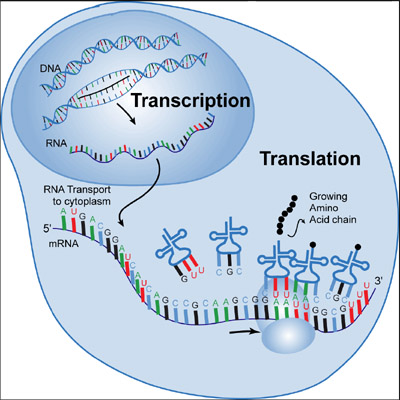
\includegraphics[height = 9cm, width = 9cm]{img/transcp_transla.jpg}
\caption{Transcription and Translation. From:  \href{http://www.tokresource.org}{tokresource.org}\label{fig:trans_trans}}
\end{center}
\end{figure}

\begin{figure}[!h]
\begin{center}
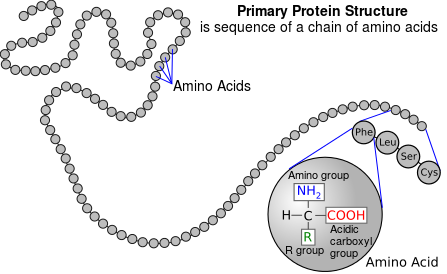
\includegraphics[ width = 8cm]{img/pro_amin.jpg}
\caption{Protein sequence. (From:  \href{http://www.wikimedia.org/}{wikimedia.org}) \label{fig:pro_se}}
\end{center}
\end{figure}

\section{Protein}
\textcolor{red}{add 1,2,3,4 structure of proteins}
Proteins are made of twenty kinds of amino acids. The function of proteins varies. The main functions of proteins can be working as antibodies, contractile proteins, enzymes, hormonal proteins, structural, storage proteins, transport proteins, etc. (\cite{white1959principles}).
In bioinformatics, we usually use FASTA format files to represent the amino acid sequences of proteins in an organism.
A FASTA file consists of protein or DNA names, description and sequences. Identifiers are preceded by a greater-than symbol "\textgreater" and the rest of the line is a description (optional). The next lines up to the next greater-than symbol contain the actual DNA or protein sequence. Figure \ref{fig:fasta} shows an example of a FASTA format. The protein name "YPR161C" follows the "\textgreater" sign. The protein sequence is given in the next five lines.


\begin{figure}
\begin{center}
\ttfamily{

	\begin{tabular}{p{2pt}p{2pt}p{2pt}p{2pt}p{2pt}p{2pt}p{2pt}p{2pt}p{2pt}p{2pt}p{2pt}p{2pt}p{2pt}p{2pt}p{2pt}p{2pt}p{2pt}p{2pt}p{2pt}p{2pt}p{2pt}p{2pt}p{2pt}p{2pt}p{2pt}p{2pt}p{2pt}}
	> & Y & P & R & 1 & 6 & 1 & C & \\ 
	T & T & G & A & C & M & T & T & G & A & C & M &T & T & G & A & C & M &V & V & V & R & N & M &\\ 
	 A & C & M &T & T & G & A & C&T & T & G & A & C & M & T & T & G  & M &T & T & G & A & C & M &\\ 
	Q & S & D& A & V & M & T & T & G & A & C & M &T & T & G & A & C & M &T & T & G & A & C & M &\\ 
	A & C & M &T & T & G & A & C & M & T & T & G & A & C & M &T & T & G & T & T & G & A & C & M &\\ 
	T & T & G & A & C & M & T & T & G & A & C & M &T & T &\\ 
	\end{tabular} \\

}
\caption{A protein in FASTA format.\label{fig:fasta}}
\end{center}
\end{figure}
\section{Protein-protein Interaction}
Proteins are some of the most important molecules in cells (\cite{schleif1993genetics}). 
They carry out most of the cellular processes. Quite often, they keep the cells functioning by interacting with other proteins in stable or transient protein complexes (\cite{eisenberg2000protein}).
This process is called protein-protein interaction (PPI). This is a vital process because of the accepted idea that PPIs are responsible for cell's behaviour under different stimuli (\cite{bader2003functional, pandey2000proteomics, schwikowski2000network}).
Protein complexes are groups of proteins that interact together to perform certain functions. Figure \ref{fig:pro_comp} shows an example of a protein complex. Protein pathways and modules are another two functional groups connected through PPIs. 
\begin{figure}[h!]
\begin{center}
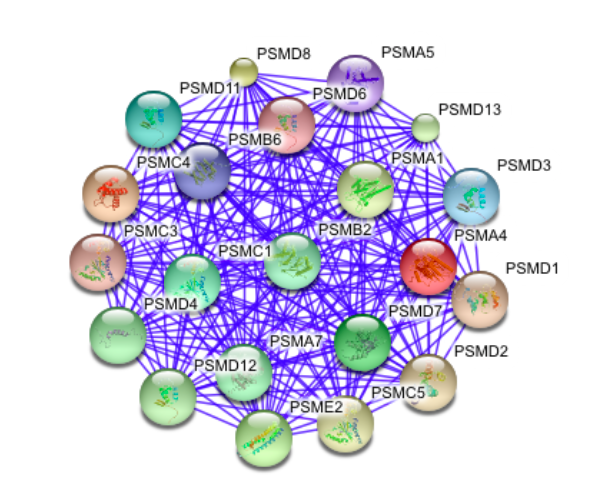
\includegraphics[height = 8cm]{img/pro_comp.png}
\caption{Protein complex. (From: bioproximity.com)  \label{fig:pro_comp}}
\end{center}
\end{figure}
 Scientists believe the reason that advanced organisms like humans are more complicated than lower organisms like the worms is not only because of large number of genes, but also because of sophisticated PPI networks \cite{pitre2008computational}. Figure \ref{fig:ppi_net} shows a map of human PPIs.
Understanding the potential of unknown proteins is becoming possible by looking into their PPI information \cite{sharan2007network}. As well, knowing PPI information helps improve the system-level understanding of molecular processes \cite{levy2008evolution}.
Therefore, understanding and mapping PPIs is an important current area of research.

\begin{figure}[h!]
\begin{center}
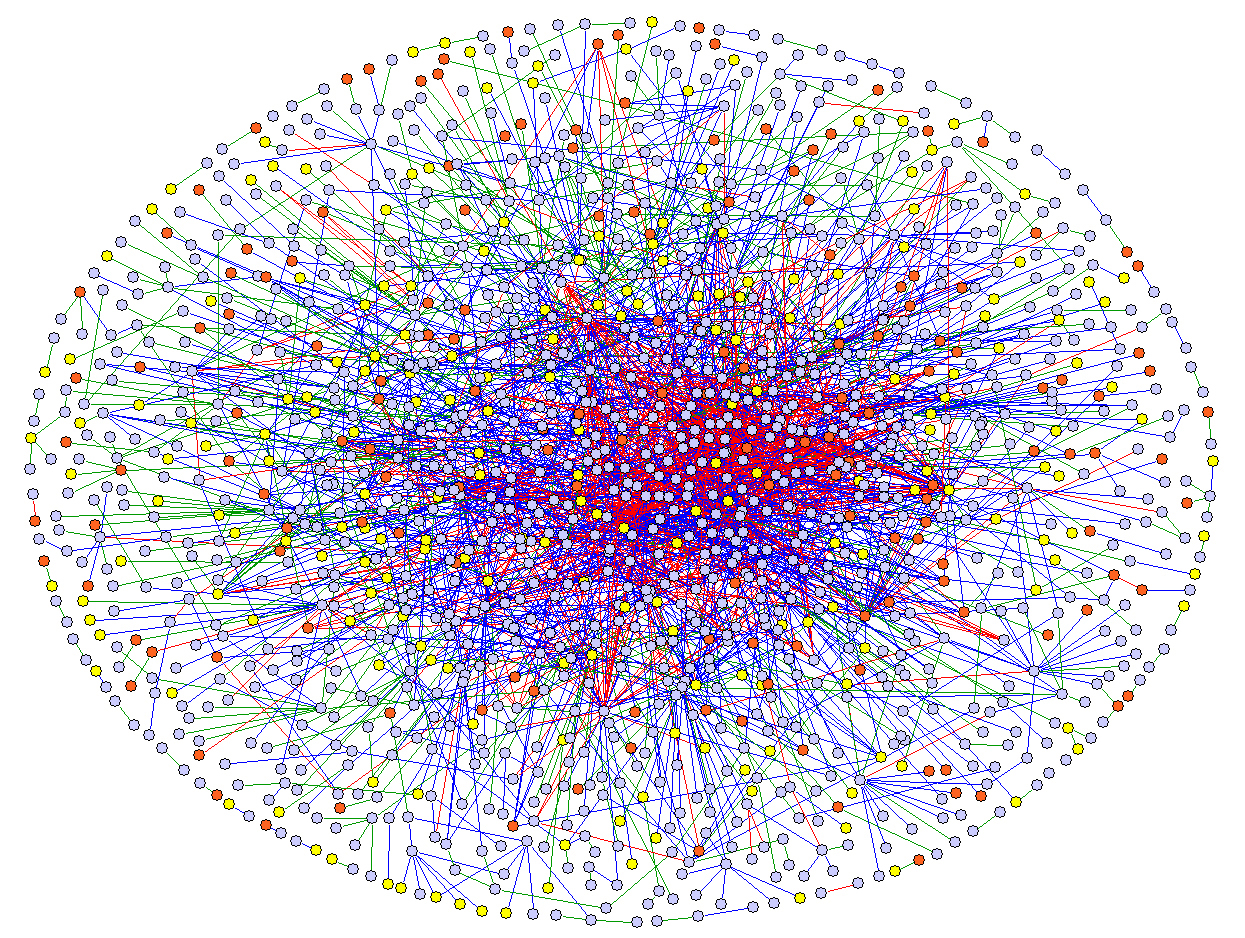
\includegraphics[height = 10cm, width = 10cm]{img/pro_inter_net.jpg}
\caption{A human protein-protein interaction network. (From: \href{https://www.mdc-berlin.de/}{www.mdc-berlin.de})  \label{fig:ppi_net}}
\end{center}
\end{figure}

However, there are a lot of unknown facts about PPIs to be discovered. For example, in a simple organism such as Saccharomyces cerevisiae, there are less than 40,000 estimated PPIs. Comparing with 19,000,000 potential interacting pair, it is believed that there is still a significant gap between known PPIs and real ones \cite{jessulat2011recent, sprinzak2003reliable}. Precise, fast and affordable protein-protein interaction prediction methods are needed.

The idea of PPI prediction is shown in Figure \ref{fig:ppi_pred}. The left part contains fours proteins and two known interactions, indicated using circles and blue lines respectively. Using those as inputs, PPI prediction methods would output a predicted interaction, indicated by the red line in the right picture. 
\begin{figure}[h!]
\begin{center}
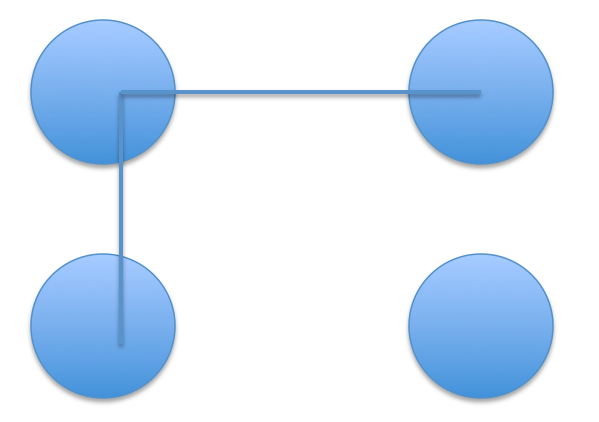
\includegraphics[width=6cm]{img/know_ppi.png}
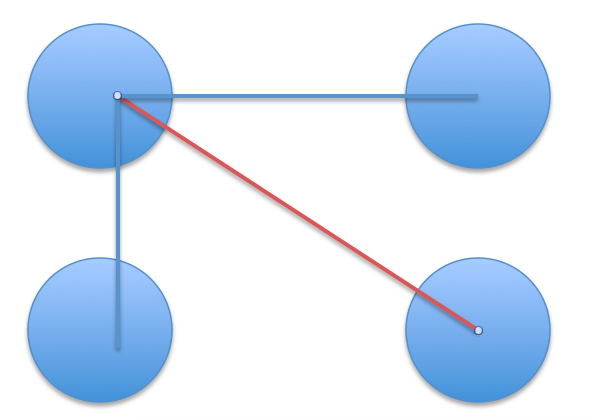
\includegraphics[width=6cm]{img/predict_ppi.png}
\end{center}
\caption{The idea of protein-protein interaction prediction.  \label{fig:ppi_pred}}
\end{figure}

There are many proposed PPI prediction methods, both experimental and computational ones. The most widely used experimental methods are Yeast two-hybrid (Y2H) \cite{fields1989novel} and Tandem affinity purification (TAP) \cite{suter2008two}. 

The yeast two-hybrid (Y2H) detects a protein interaction by telling the signal generated by the DNA-binding domain (DBD) and the activation domain (AD). There are several drawbacks of this approach. First, it can only detect PPIs within the nucleus. Second, it can only detect one interaction at a time, which is quite inefficient. Also, the false positive and false negative rates are high \cite{stephens2000use, semple2002jury}.

Tandem affinity purification (TAP) detects protein interactions by attaching a tag to the protein complex. After tagging, the complex is washed twice to remove the tag and unstable bindings. Isolated interacting proteins can be found if there are some. After washing, the mass spectrometry or other methods will be used to detect remaining proteins. The remaining ones are marked as interacting proteins \cite{rigaut1999generic}. A major advantage of the TAP approach is that it can detect interactions of protein complexes (more than two proteins), even without the interacting pattern. However, the "tag" added to proteins is itself a disadvantage. It might become a confounding factor in a way that changes the interacting process. Also, some real interactions can be washed away during two times of washing, thus increasing the false negative rate \cite{jessulat2011recent}.

 The experimental approaches are generally time and labour consuming. Also, they have the limitation of being unable to detect some protein complexes. In addition, the false positive rate and false negative rate of those approaches are high (\cite{pitre2006pipe}). Due to these disadvantages, computational approaches are proposed. Currently, there are mainly six kinds of computational PPI prediction approaches: genomic approach, evolutionary relationship approach, protein structure approach, domain approach, network analysis approach, and primary protein structure approach \cite{jessulat2011recent}. Our focus will be on the primary protein structure, or sequence based, approaches, and we give more details in the next chapter.
 
\section{Protein-protein Interaction Binding Sites}
Proteins interact with each other by binding together. Figure \ref{fig:ppi_bind} shows two binding proteins. The connecting parts between the blue protein and the red protein are the two binding sites of this interaction. These binding sites/ sub-sequences mediate this interaction.
\begin{figure}[h!]
\begin{center}
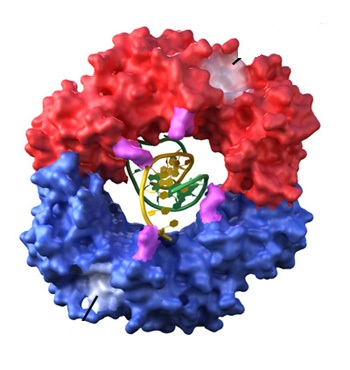
\includegraphics[width=6cm]{img/binding_sites.jpg}
\end{center}
\caption{Protein-protein interaction binding sites. (From: http://pdbj.org/eprots/) \label{fig:ppi_bind}}
\end{figure}

Knowing the binding sites help scientists understand cellular pathways better. However, the current protein interface predictors need improvements. Experimental approaches often report wrong binding
sites because of the wet lab processes, while computational approaches often require data which is not available at the proteome scale. \cite{amos2011binding}.

\begin{figure}[ht]
\begin{center}
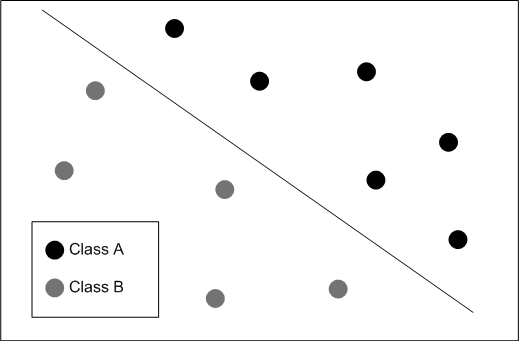
\includegraphics[height = 9cm, width = 9cm]{img/linear-classifier.png}
\caption{A long memory time series\label{ts1}}
\end{center}
\end{figure}

% Here's a table.
% \begin{table}[ht]
% \begin{center}
% \begin{tabular}[ht]{|c|lr|c|} 
%c stands for centre, l for left, r for right; the | puts lines in between, and the hline puts a horizontal line in
% \hline
% $n$ & $\alpha$ &$n\alpha$ & $\beta$\\
% \hline
% 1 & 0.2 & 0.2 & 5\\
% \hline
% 2 & 0.3 & 0.6 & 4\\
% \hline
% 3 & 0.7 & 2.1 & 3\\
% \hline
% \end{tabular}
% \caption{A random table \label{tab1}}
% \end{center}
% \end{table}

% \begin{eqnarray}
% y &=& mx + b \label{eq1}\\
% &=& ax+ c
% \label{eq2}
% \end{eqnarray}

% This is an un-numbered equation, along with a numbered one. 
% \begin{eqnarray}
% u &=& px \nonumber\\
% p &=& P(X=x) \label{eqn3}
% \end{eqnarray}

% Look at Table \ref{tab1} and Figure \ref{ts1} and equations \ref{eq1},  \ref{eq2}, and \ref{eqn3}.

% Let's do some matrix algebra now.

% \begin{equation}
% det\left(\left|\begin{array}{ccc} 2 & 3 & 5\\
% 4 & 4 & 6\\
% 9 & 8 & 1
% \end{array}\right|\right) = 42
% \end{equation}

% In the equation and eqnarray environments, you don't need to have the dollar sign to enter math mode.

% \begin{eqnarray}
% \alpha = \beta_1 \Gamma^{-1}
% \end{eqnarray}

% This is citing a reference ~\cite{zhang2019scriber}.  This is citing another ~\cite{zhang2019scriber}.  Nobody said something ~\cite{zhang2019scriber}.

\chapter{Protein-protein Interaction Prediction: SPRINT}
This chapter descibes two of our publications SPRINT \cite{li2017sprint, li2020predicting}, a sequence based protein-protein interaction site prediction program. We first introduce the prerequisites used in SPRINT as well as the state-of-the-art methods. Then we describe both the algorithm and the implementation of SPRINT in details.  Last, we compare DELPHI with five state-of-the-art programs on seven datasets showing that it is more accurate while running orders of magnitude faster and using very little memory.
\section{Background}
\subsection{Basic Notions and Definitions}
\subsubsection{BLAST seeds}
\subsubsection{Spaced seeds}
\subsubsection{Multiple spaced seeds}
\subsubsection{Substitution matrix}
\subsubsection{Interactome prediction}
\subsection{Previous Methods}
As shown in Table \ref{table_experimental_ppi_pred}, various experimental techniques for identifying PPIs have been developed, most notably high throughput procedures such as two-hybrid assay and affinity systems \cite{shoemaker2007deciphering}. Such methods are time and labor intensive and have a high rate of error. Therefore, a variety of computational methods have been designed to help predicting PPIs, employing sequence homology, gene co-expression, phylogenetic \cite{shoemaker2007deciphering, liu2012proteome, zahiri2013computational}.
profiles, etc. [3–5].
\begin{table}[htbp]
\begin{center}
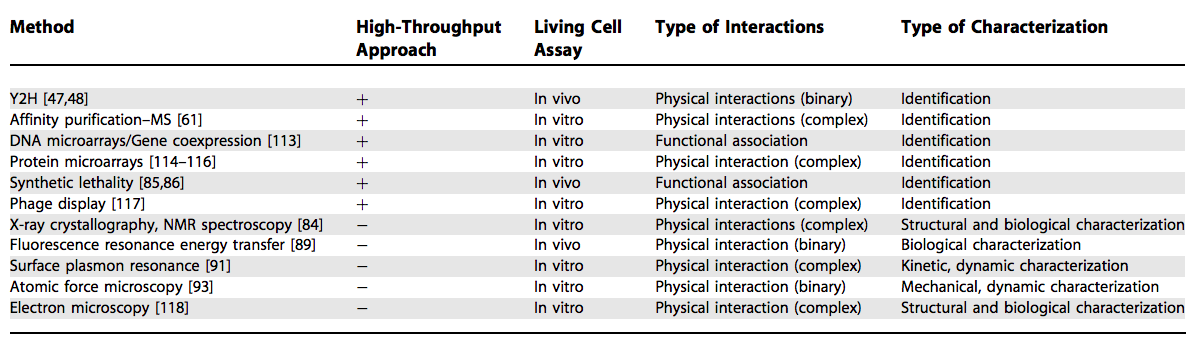
\includegraphics[ width = 16cm]{img/experimental_PPI_identification.png}
\caption{Experimental methods for PPI identification (From \cite{shoemaker2007deciphering}). High-throughput methods are marked with + in the second column. The fourth column shows whether the method on physically interacting proteins in a complex (‘‘complex’’) or only pairwise interactions (‘‘binary’’).   \label{table_experimental_ppi_pred}}
\end{center}
\end{table}

In general, based on the input, computational methods can be classified into two categories: sequence based and structure based \cite{zhang2018review}. Sequence based methods are faster and more universal because not all proteins have structures available. 

\subsubsection{SigProd}
\subsubsection{PIPE}
\subsubsection{Ding's}
\section{Methods}
\subsection{SPRINT Overview}
\subsection{Training Data Preparation}
\subsection{Detecting Similarities}
\subsubsection{Seed representations}
\subsubsection{Storing sub-sequences}
\subsubsection{Hash table and hash function}
\subsection{Predicting Interactions}
\subsubsection{Post-processing similarities}
\subsubsection{Scoring function}
\subsubsection{Fast prediction}
\subsection{Implementations}
\section{Results}
\subsection{Datasets}
\subsection{Evaluation Scheme}
\subsection{Comparative Analysis on Park \& Marcotte’s Datasets}
\subsection{Comparative Analysis on Seven Human Datasets}
\subsection{Comparative Analysis on Human Interactome Prediction}
\subsection{Availability}
\section{Conclusion}
% \section{Basic Theorems}
% \begin{theorem}
%  $e^{i\pi} = -1$ \label{eipi}
% \end{theorem}
\chapter{SPRINT \label{chap_3}}
This chapter describes our two publications regarding SPRINT (Scoring PRotein INTeractions) \cite{li2017sprint, li2020predicting}, a sequence based protein-protein interaction site prediction program. We first introduce the prerequisites used in SPRINT as well as the state-of-the-art methods. Then we describe both the algorithm and the implementation of SPRINT in details.  Last, we compare DELPHI with five state-of-the-art programs on seven datasets showing that it is more accurate while running orders of magnitude faster and using very little memory.
\section{Background}
In addition to the deep learning prerequisites introduced in Section \ref{set_AI_in_bioinfor}, we explain some preliminary algorithmic concepts used in the SPRINT algorithm in this section.
\subsection{Similarity Search}
Similarity search is a task to detect identical or similar segments among sequences. It is a routinely performed task DNA or protein sequences. Many bioinformatics programs highly depend on similarity search, and quite a few algorithms have been proposed for this task. 

The Smith-Waterman algorithm \cite{smith_waterman_1981} was proposed in the early 80's. This classic dynamic programming algorithm detects the optimal local alignment between two sequences. It guarantees to find the best solution, and that comes with the price of high time complexity. As shown in Figure \ref{fig_smith_waterman}, the Smith-Waterman algorithm works as two steps: Filling the scoring matrix and tracing back the optimal alignment. The value $S[i,j]$ in the position  $(i,j)$ is determined by three values around it: $S[i-1,j-1]$, $S[i-1,j]$, and $S[i,j-1]$. The detailed algorithm and analysis can be seen in \cite{smith_waterman_1981}. The worst time complexity is $O(mn)$ where $m$ and $n$ are the lengths of two sequences. This computationally expensive algorithm was soon overwhelmed by the amount of increasing biological data.

\begin{figure}[h!]
     \centering
     \begin{subfigure}[b]{0.45\textwidth}
         \centering
         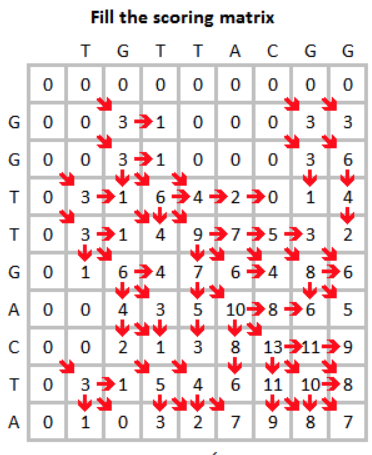
\includegraphics[width=\textwidth]{img/Smith_waterman_fill_matrix.png}
        %  \caption{$y=3sinx$}
        %  \label{fig_three sin x}
     \end{subfigure}
     \hfill
     \begin{subfigure}[b]{0.45\textwidth}
         \centering
         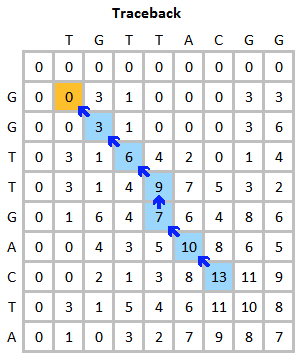
\includegraphics[width=\textwidth]{img/Smith_waterman_backtra.png}
        %  \caption{$y=5/x$}
        %  \label{fig_five over x}
     \end{subfigure}
        \caption[The Smith-Waterman algorithm.]{The Smith-Waterman algorithm. From wikipedia.org.}
        \label{fig_smith_waterman}
\end{figure}

\subsubsection{BLAST Seeds}
Heuristic algorithms were proposed aiming to detecting similarities much faster and at the same time, detecting most of the similarities.

The most noticeable algorithm and its suite is the the BLAST (Basic Local Alignment Search Tool) family \cite{Altschul90_BLAST, altschul1997PSI_BLAST}. BLATS serves as part of the pipelines for thousands of programs. The two papers together have had 157,399 citations till May 2020. 

The key process in BLAST is called hit-and-extension. When identifying similarity, BLAST requires first short consecutive matches between two strings. Then the matched region extends to both the left and the right side to form a longer local alignment. This extension stops until the similarities of the detected region drops below a threshold. The default number for DNA sequences is eleven consecutive matches. Denoting the matches by 1's we obtain what is called a consecutive seed: 11111111111. A pair of identical consecutive matches is called a hit. The similarity grows from the consecutive matches therefore they are called the seed. A seed often is used to refer to the way these eleven positions are selected.

Figure \ref{fig_BLAST} shows an example of the hit-and-extension algorithm. When a hit is detected by the consecutive seed, marked with red color, BLAST extends this hit towards both sides (blue) until certain amount of mismatches are detected. 
\\
\begin{figure}[h!]
\begin{center}
\setlength{\tabcolsep}{4.5pt}
\ttfamily{
\begin{tabular}{ccccccccccccccccccccccccccc}
\ & \ & \ & \ & \ & \ & \ & \ & \textbf{|} & $\leftarrow$ & \ & \ & \ & h & i & t & \ & \ & $\rightarrow$ & \textbf{|} & \ & \ & \ & \ & \ & \ & \\
T & T & G & A & C & \textcolor{blue}{A} & \textcolor{blue}{T} & \textcolor{blue}{G} & \textcolor{red}{T} & \textcolor{red}{C} & \textcolor{red}{T} & \textcolor{red}{C} & \textcolor{red}{T} & \textcolor{red}{A} & \textcolor{red}{G} & \textcolor{red}{T} & \textcolor{red}{G} & \textcolor{red}{A} & \textcolor{red}{G} &\textcolor{red}{ T} & \textcolor{blue}{C} & \textcolor{blue}{T} & \textcolor{blue}{C} & T & A & T &\\ 
| & | & \ & \ & \ & | & | & | & | & | & | & | & | & | & | & | & | & | & | & | & | & | & | & \ & \ & \ & \\ 
T & T & A & C & T & \textcolor{blue}{A} & \textcolor{blue}{T} & \textcolor{blue}{G} & \textcolor{red}{T} & \textcolor{red}{C} & \textcolor{red}{T} & \textcolor{red}{C} & \textcolor{red}{T} & \textcolor{red}{A} & \textcolor{red}{G} & \textcolor{red}{T} & \textcolor{red}{G} & \textcolor{red}{A} & \textcolor{red}{G} &\textcolor{red}{ T} & \textcolor{blue}{C} & \textcolor{blue}{T} & \textcolor{blue}{C} & A & T & G &\\ 
\ & \ & \ & \ & \ & \ & \ & \ & 1 & 1 & 1 & 1 & 1 & 1 & 1 & 1 & 1 & 1 & 1 & 1 & \ & \ &\  & \ & \ & \ & \\
\ & \ & \ & \ & \ & \textbf{|} & $\leftarrow$ & \tiny {\textbf{ext.}} & \ & \ & \ & \ & \ & \ & \ & \ & \ & \ & \ & \ & \tiny{\textbf{ext.}} & $\rightarrow$ &\textbf{|}  & \ & \ & \ & \\
\\
\end{tabular} \\
}
\caption[An example of the hit-and-extend algorithm in BLAST]{An example of the hit-and-extend algorithm in BLAST. A hit (red region) is identified first and then extended (blue region) to form a longer local alignment.  \label{fig_BLAST}}
\end{center}
\end{figure}

To reduce the time complexity, fast identification hits is usually implemented by indexing sequences in data structures like hash table, suffix array, or a suffix tree. Details of the SPRINT indexing implementation will be discussed in Section \ref{sec_detect_simi}. 

The sensitivity of a seed is defined by its probability of finding similarities. The length of the consecutive seed in BLAST determines the sensitivity and the speed of the program. In order to detecting more hits, i.e. higher sensitivity, shorter seeds are needed, but shorter seeds also means higher time complexity.

\subsubsection{Spaced Seeds}
PatternHunter proposed \cite{Ma02_PatternHunter} the idea of spaced-seed. Denote the five consecutive matches of a BLAST seed by 11111; this is called a consecutive seed of weight five. Spaced  seeds consists of matches interspersed by "don’t care" positions. Matches positions are denoted by 1, and "don't care" positions are denoted by *, sometimes by 0. here is an example of such a spaced seed of weight 11 and length 18: 111*1**1*1**11*111. A spaced match requires only the letters in positions corresponding to 1’s in the seed to match. Figure \ref{fig_hit_spaced_seed} shows an example of a hit using the spaced-seed. The match positions requires identical characters in two sequences while the "don't care" positions do not.

\begin{figure}[h!]
\begin{center}
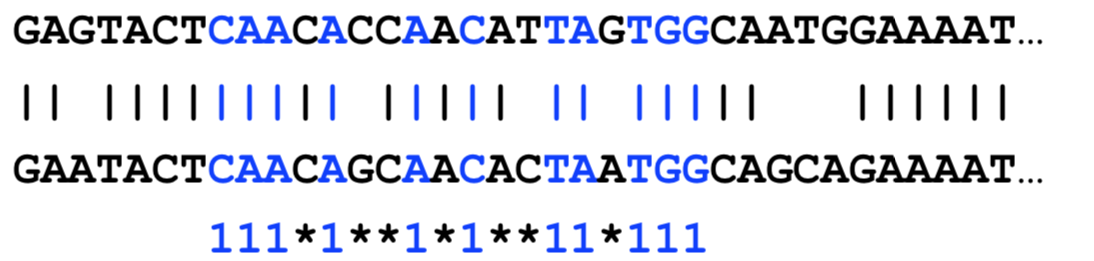
\includegraphics[height =3.5 cm]{img/spaced_seed_hit.png}
\caption[A hit of a spaced-seed]{A hit of a spaced-seed. 1's in the seed require a match in the two target sequences (blue), but the * positions do not care whether the corresponding positions in the two sequences match or not.  \label{fig_hit_spaced_seed}}
\end{center}
\end{figure}

A spaced-seed is more sensitive than a consecutive seed of the same weight while maintaining the same time complexity. For random sequences $S$ and $T$ with lengths $m$ and $n$, the expected number of hits for weight $w$, length $l$ seed is $(m-l+1)(n-l+1)4^{-w}$. Usually $l$ is much shorter than $m$ and $n$, this value is approximately $4^{-w}mn$. In other words, the expected number of hits in random regions only depends on the weight of the seed, but not the shape of the seed. Therefore, two seeds, one consecutive and one spaced, of the same weight have the same number of expected hits. That is the reason that time complexity does not change when adding "don't" care positions in the seed.

Spaced-seeds outperform consecutive seeds in sensitivity because they avoid hit clustering. As shown in Figure \ref{seeds}, after having a hit, the consecutive seed requires only one additional match when shifting one position to the right. This way, a long similarity region will be hit many times. In contrast, the spaced seed requires six matching characters when shifting one position. As stated above, the total number of hits using two seeds of the same weight is the same, spaced seeds have their hits much better distributed.  Because the hits of a spaced seed are less clustered together, more regions will be hit, thus increasing the probability of finding similarities. As shown in Fig. \ref{fig_seed_sens}, a spaced-seed of weight 11 is more sensitive than a BLAST seed with weight 11. It  is even higher than a BLAST seed with weight 10.
\begin{figure}[h!]
\begin{center}
\setlength{\tabcolsep}{2pt}
\ttfamily{
\begin{tabular}{ccccccccccccccccccccccccccccccccccccccc}
\textcolor{red}{C} & \textcolor{red}{G} & \textcolor{red}{T} & \textcolor{red}{C} & \textcolor{red}{A} & \textcolor{red}{A} & \textcolor{red}{G} & \textcolor{red}{A} & \textcolor{red}{C} & \textcolor{red}{T} & \textcolor{red}{T} & ? & \ & \ & \ & \ & \ &  \ & \ &\textcolor{red}{G} & \textcolor{red}{A} & \textcolor{red}{G} & ? & \textcolor{red}{C} & ? &? &  \textcolor{red}{T} & ? & \textcolor{red}{G} & ? & ? & \textcolor{red}{A} & \textcolor{red}{C} & ? & \textcolor{red}{T} & \textcolor{red}{T} & \textcolor{red}{C} & ? & \\
\textcolor{red}{|} & \textcolor{red}{|} & \textcolor{red}{|} & \textcolor{red}{|} & \textcolor{red}{|} & \textcolor{red}{|} & \textcolor{red}{|} & \textcolor{red}{|} & \textcolor{red}{|} & \textcolor{red}{|} & \textcolor{red}{|} & ? & \ & \ & \ &  \ & \ & \ & \ &\textcolor{red}{|} & \textcolor{red}{|} & \textcolor{red}{|} & ? & \textcolor{red}{|} & ? &? &  \textcolor{red}{|} & ? & \textcolor{red}{|} & ? & ? & \textcolor{red}{|} & \textcolor{red}{|} & ? & \textcolor{red}{|} & \textcolor{red}{|} & \textcolor{red}{|} & ? &\\
\textcolor{red}{C} & \textcolor{red}{G} & \textcolor{red}{T} & \textcolor{red}{C} & \textcolor{red}{A} & \textcolor{red}{A} & \textcolor{red}{G} & \textcolor{red}{A} & \textcolor{red}{C} & \textcolor{red}{T} & \textcolor{red}{T} & ? & \ & \ & \ & \ & \ & \ & \ & \textcolor{red}{G} & \textcolor{red}{A} & \textcolor{red}{G} & ? & \textcolor{red}{C} & ? &? &  \textcolor{red}{T} & ? & \textcolor{red}{G} & ? & ? & \textcolor{red}{A} & \textcolor{red}{C} & ? & \textcolor{red}{T} & \textcolor{red}{T} & \textcolor{red}{C} & ? &\\
1 & 1 & 1 & 1 & 1 & 1 & 1 & 1 & 1 & 1 & 1 & \ & \ & \ & \ & \ & \ &  \ & \ &1 & 1 & 1 & * & 1 & * &* &  1 & * & 1 & * & * & 1 & 1 & * & 1 & 1 & 1 & \\
\ &1 & 1 & 1 & 1 & 1 & 1 & 1 & 1 & 1 & 1 & \textcolor{red}{1} &  \ & \ &\ & \ & \ & \ & \ & \ & 1 & 1 & \textcolor{red}{1} & * & \textcolor{red}{1} & * &* &  \textcolor{red}{1} & * & \textcolor{red}{1} & * & * & 1 & \textcolor{red}{1} & * & 1 & 1 & \textcolor{red}{1} &\\
\end{tabular} \\
}
\caption[Consecutive seed and spaced seed]{Consecutive seed (left) and spaced seed (right). The red 1's are new matches required for a hit at the next position; it is much easier for the consecutive seed to have consecutive hits, hence its hits are more clustered  than those of the spaced seed.}
\label{seeds}
\end{center}
\end{figure}

\begin{figure}[h!]
\begin{center}
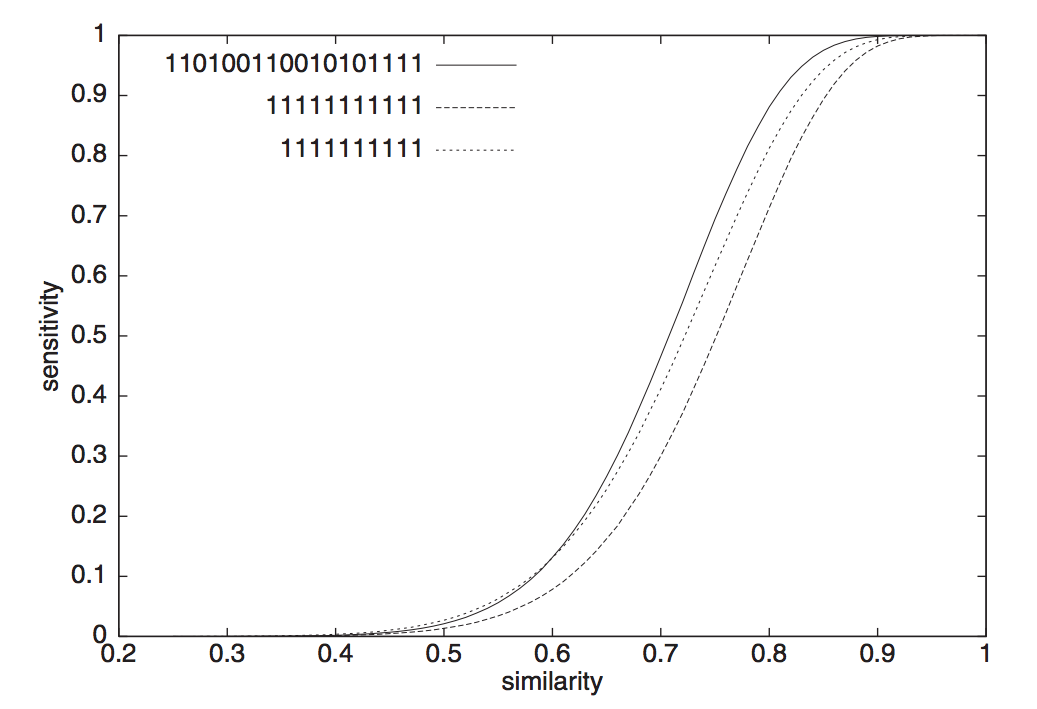
\includegraphics[ height= 7cm]{img/seed_sens.png}
\caption[The sensitivity comparison of three spaced-seed and BLAST seed]{The sensitivity comparison of three spaced-seed and BLAST seed. (From \cite{Ma02_PatternHunter}).    \label{fig_seed_sens}}
\end{center}
\end{figure}

\subsubsection{Multiple Spaced Seeds \label{sec_multiple_spaced_seed}}
Different spaced-seeds detect different similarity. PatternHunterII \cite{Li04_PatternHunterII} proposed the idea of combining multiple spaced-seeds to detect more similarities. A sensitivities comparison is shown in Figure \ref{fig_multi_spaced_seed}. The x-axis, similarity, denotes the percentage of identities in the similar region, and the y-axis, sensitivity, is the probability of having a hit, in the given region. The first observation is that the increment of the seed number improves the sensitivity. It is also notable that typically, doubling the number of seeds gains better sensitivity than decreasing the weight by 1.
\begin{figure}
\begin{center}
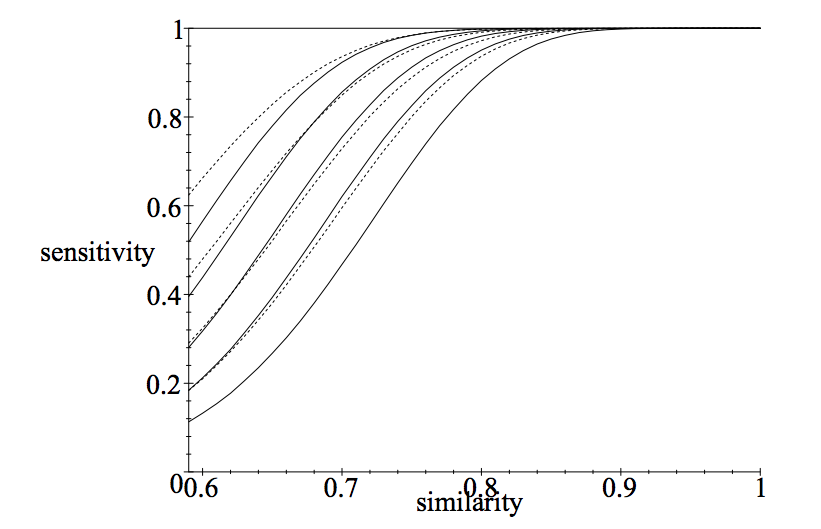
\includegraphics[ height= 7cm]{img/multi_spaced_seeds.png}
\caption[The sensitivity comparison on multiple spaced-seed]{The sensitivity comparison on multiple spaced-seed.  From low to high, the solid curves are the sensitivity of multiple spaced seed of weight 11. Denote the number of seeds as $k$, here $k=1,2,4,8,16$. 
The dashed curves are the sensitivity of single optimal spaced-seed of weight 10, 9, 8, 7. (From \cite{Li04_PatternHunterII}).    \label{fig_multi_spaced_seed}}
\end{center}
\end{figure}

Because of the advantage in sensitivity, SPRINT adopts the multiple spaced-seeds. The next natural step is to pick the shape of the seeds. Computing optimal seeds is a hard problem. Even the heuristic algorithms are exponential, except for SpEED \cite{ilie2007multiple, ilie2011speed}. We have thus used SpEED to compute the multiple spaced seeds to be used in our PPI prediction program. 

\subsubsection{Substitution Matrix}
In bioinformatics and evolutionary biology, a substitution matrix describes the rate at which one character in a sequence changes to other character states over time. The similarity between sequences depends on their divergence time and the substitution rates as represented in the matrix. Substitution metrics like PAM and BLOSUM are often used as similarity measurement for protein sequences \cite{eddy2004_BLOSUM_PAM}, and thus they are sometimes called similarity matrices. An example, the BLOSUM62 matrix is shown in Figure \ref{fig_BLOSUM62}.

\begin{figure}[h!]
\begin{center}
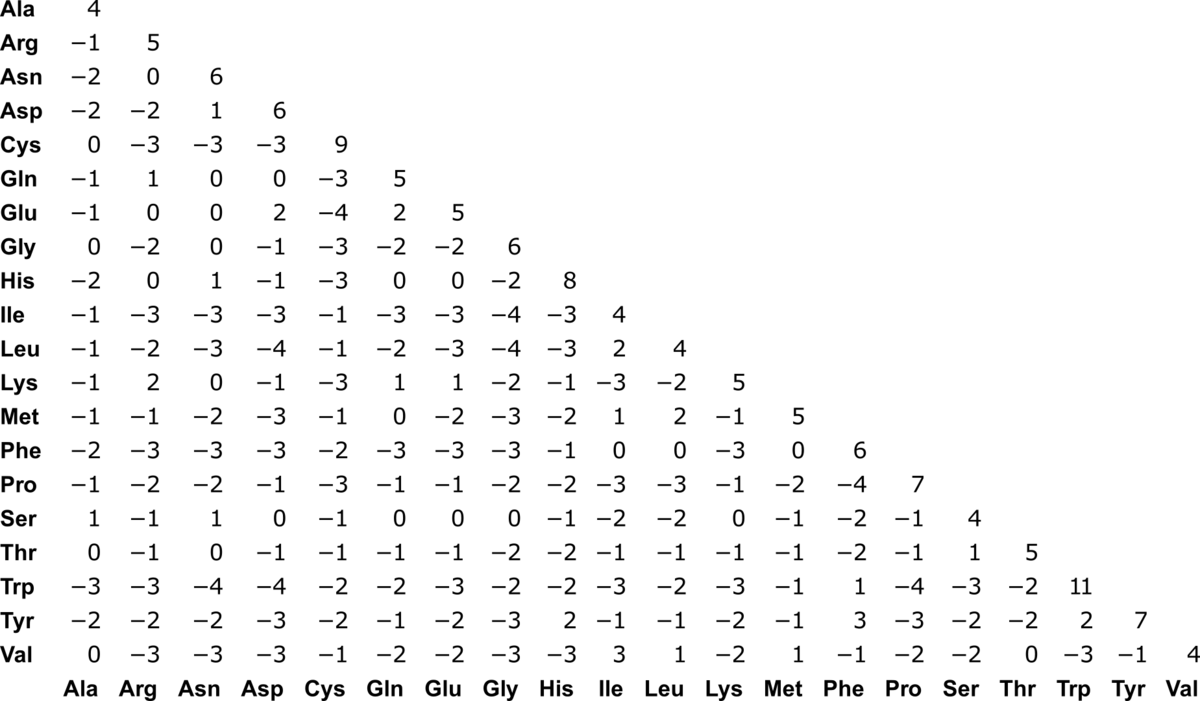
\includegraphics[ height= 7cm]{img/BLOSUM62.png}
\caption[The BLOSUM62 matrix]{An example of substitution matrix, the BLOSUM62 matrix. BLOSUM 62 is a matrix calculated from comparisons of sequences with a pairwise identity of no more than 62\%. From \text{wikipedia.org}    \label{fig_BLOSUM62}}
\end{center}
\end{figure}

\subsubsection{Interactome Prediction}
The PPI prediction problem, interactome prediction means to score every pair in a proteome of an organism. Denote the total number of protein sequences in an organism as $P$, its interactome has $(1+P)\times P\div 2$ interactions. This is a relatively big number for advanced organisms. For instance, human has about 20,000 proteins, and human's interactome has $(1+20000) \times 20000\div 2 = 200,010,000$ interactions to predict. Comparing to the PPI site prediction problem, which only involves the computation on $P$ sequences, the amount of computation is much higher in the PPI prediction problem.

\subsection{Previous Methods}
As shown in Table \ref{table_experimental_ppi_pred}, various experimental techniques for identifying PPIs have been developed, most notably high throughput procedures such as two-hybrid assay and affinity systems \cite{shoemaker2007deciphering}. 
\begin{table}[h!]
\begin{center}
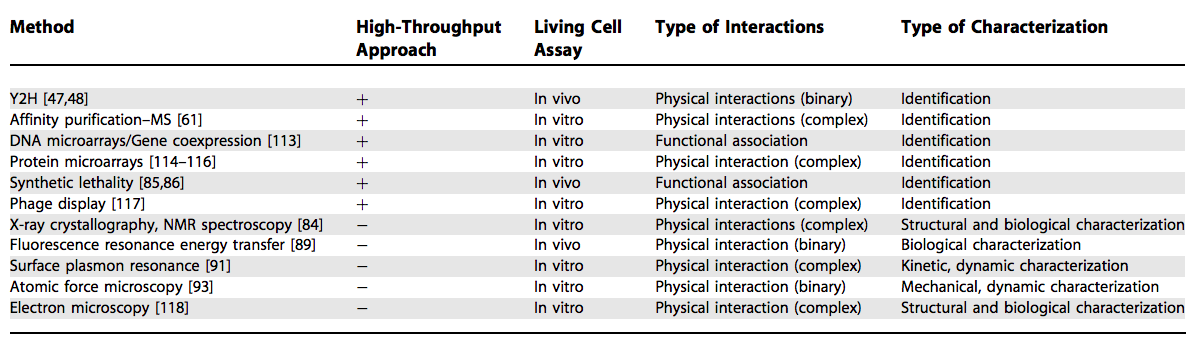
\includegraphics[ width = 16cm, height= 7cm]{img/experimental_PPI_identification.png}
\caption[Experimental methods for PPI identification]{Experimental methods for PPI identification. High-throughput methods are marked with + in the second column. The fourth column shows whether the method on physically interacting proteins in a complex (‘‘complex’’) or only pairwise interactions (‘‘binary’’). (From \cite{shoemaker2007deciphering})  \label{table_experimental_ppi_pred}}
\end{center}
\end{table}

The yeast two-hybrid (Y2H) approach was proposed by Suter et al. \cite{fields1989novel}. It detects a protein interaction by telling the signal generated by the DNA-binding domain (DBD) and the activation domain (AD) \cite{suter2008two}. Figure \ref{E_M1} shows the basic procedure of the Y2H approach. To detect whether protein 1 (green) and protein 2 (red) interact or not, then DBD and AD are bound, each to one of the proteins. The DBD and AD will connect together only when protein 1 and protein 2 interact with each other. When DBD and AD connect, a reporter will be generated. Thus, protein 1 and protein 2 are interacting if a reporter is detected, and vice versa \cite{suter2008two}.
\begin{figure}[h!]
\begin{center}
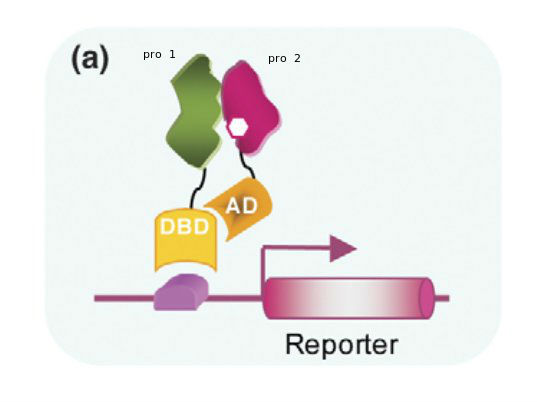
\includegraphics[height =7 cm, width = 9cm]{img/E_M1.jpg}
\caption[The Y2H approach]{The Y2H approach. To verify is protein 1 and 2 interact, DBD and AD are attached to them. If the two proteins interact, DBD and AD will bond and a reporter will be generated. The interaction is detected if the reporter is detected., From: \cite{suter2008two} \label{E_M1}}
\end{center}
\end{figure}

Another widely used experimental approach is tandem affinity purification (TAP), which was invented by Rigaut et al. \cite{rigaut1999generic}. It can detect protein complex interaction by adding a "tag" to target proteins. Figure \ref{E_M2} shows the general process of TAP. If we want to test whether interaction exists between protein $A$ and protein $B$, a tag is added to protein $A$. After tagging, the complex is washed twice to remove the tag and unstable bindings. Isolated interacting proteins can be found if there are some. After washing, the mass spectrometry or other methods will be used to detect remaining proteins. The remaining ones are marked as interacting proteins \cite{rigaut1999generic}.
\begin{figure}[h!]
\begin{center}
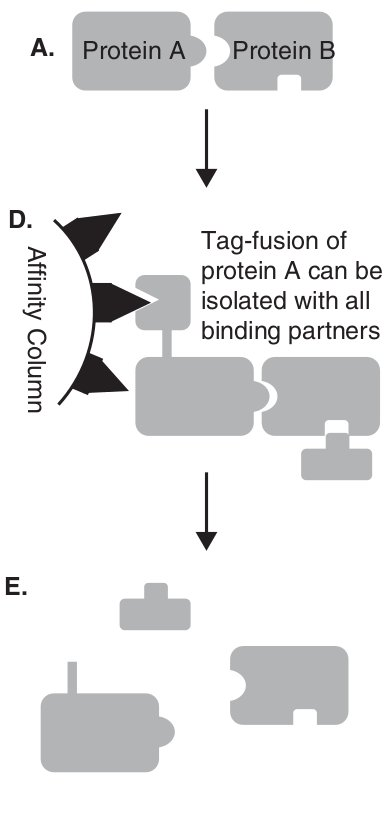
\includegraphics[height =9 cm, width = 6cm]{img/E_M2.jpeg}
\caption[Tandem affinity purification]{Tandem affinity purification. To verify if Protein A and B interact, a tag is linked to Protein A. A is able to bind the matrix in the affinity column. Molecules that bind with Protein A will also remain in the column. The second wash flushes all molecules, and those molecules considered Protein A's interaction parterner. From: \cite{jessulat2011recent} \label{E_M2}}
\end{center}
\end{figure}

Experimental methods are time and labor intensive and have a high rate of error. Therefore, a variety of computational methods have been designed to help predicting PPIs, employing sequence homology, gene co-expression, phylogenetic \cite{shoemaker2007deciphering, liu2012proteome, zahiri2013computational}.
profiles, etc. [3–5].


In general, based on the type input, computational methods can be classified into two categories: sequence based and structure based \cite{zhang2018review}. Sequence based methods \cite{ Martin05_PPIpred,Pitre06_PIPE,Shen07_PPIpred,Guo08_PPIpred,yu2010predicting, xia2010predicting,shi2010predicting, guo2010pred_ppi,zhang2011adaptive, liu2012spps, yousef2013novel,zahiri2013ppievo, zahiri2014locfuse, you2015detecting, hamp2015evolutionary, jia2015prediction, huang2015using,   you2015predicting, hamp2015more, ding2016predicting,gao2016ens, huang2016sequence, an2016using,you2017improved, hashemifar2018predicting, chen2019multifaceted, chen2019protein} are faster and more universally applicable because comparing to proteins structures, much more protein sequences are available. Here we introduce several state-of-the-art sequence based PPI prediction methods. One of them is traditional algorithmic, and the rest employs machine learning algorithms.

\subsubsection{PIPE}
PIPE (Protein Interaction Prediction Engine)\cite{Pitre06_PIPE} is one of the most widely known traditional algorithmic methods. It predicts interactions based on re-occurring short sub-sequences in an existing interaction database. The  four major steps of PIPE are shown in Figure \ref{fig_PIPE}.
\begin{figure}[h!]
\begin{center}
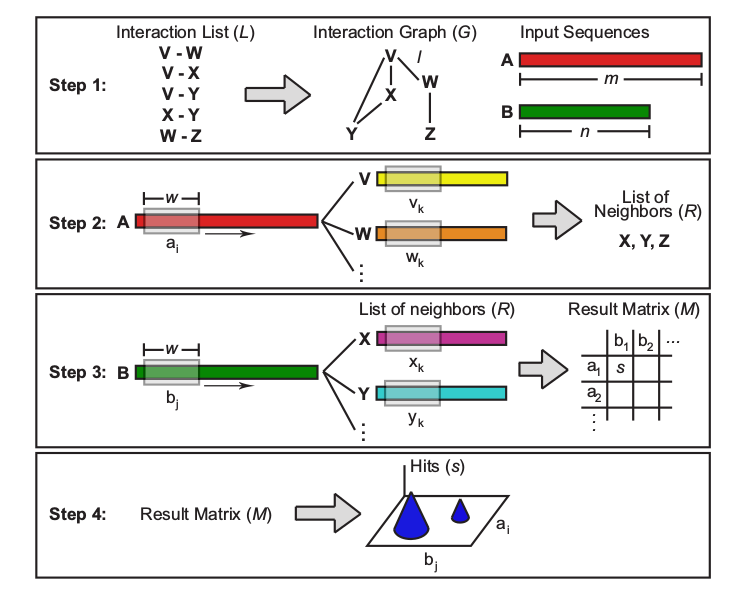
\includegraphics[height =13 cm]{img/PIPE_procedure.png}
\caption[The algorithm of PIPE]{The algorithm of PIPE. Step 1: building interaction graph from interaction database. Step 2: detecting similar sub-sequences for input $A$. Step 3: detecting similar sub-sequences for input $B$ and build the result matrix for ($A, B$). Step 4: outputing the result based on the result matrix. (From: \cite{Pitre06_PIPE} ) \label{fig_PIPE}}
\end{center}
\end{figure}
The input is a protein pair ($A$, $B$), and the output is the probability of $A$ and $B$ interact. It first puts a 20-sized window $w$ on top of $A$, then compares $w$ with every 20-sized piece in the protein sequence database. PIPE compares the similarity between two 20-sized pieces using PAM120 matrix. If the score between the two pieces are higher than a threshold (default: 35), they are considered as similar pieces. All proteins that contain similar piece with protein $A$, will be stored in a set $R$. 

Based on the interaction database, all proteins that interact with the proteins in $R$, are denoted as Neighbors ($R$). PIPE will then put a 20-sized window $w$ on protein $B$. It compares every piece in $B$ with every 20-sized piece in Neighbors($R$).

A result matrix $M$ is used to denote the score of the query ($A$, $B$). The size of the matrix is length of $A$ times length of $B$. For example, protein $A$ is similar with $C$ at position $i$, and protein $B$ is similar with $D$ at position $j$. We also know that $C$ and $D$ interact from the database, then we will increase the score of $M$($i$, $j$) by one.

In the end, the height of the highest peak in the matrix is the score for query ($A$, $B$). If the score is higher than a set threshold, PIPE will claim $A$ and $B$ interact.

The pseudocode of PIPE is shown in Figure \ref{fig_pseudocode_pipe}. The time complexity of this algorithm is $O(P^3L^2)$ where $P$ is the number of proteins and $L$ is the average protein length. If the human interactome prediction (20117 proteins with average length 557) needs to be performed using a computer that does $10^9$ operations per second, the theoretical estimated running time for PIPE is $(20117^3*557^2)/10^9$s $\approx 80 $ years.  

\begin{figure}[h!]
\begin{center}
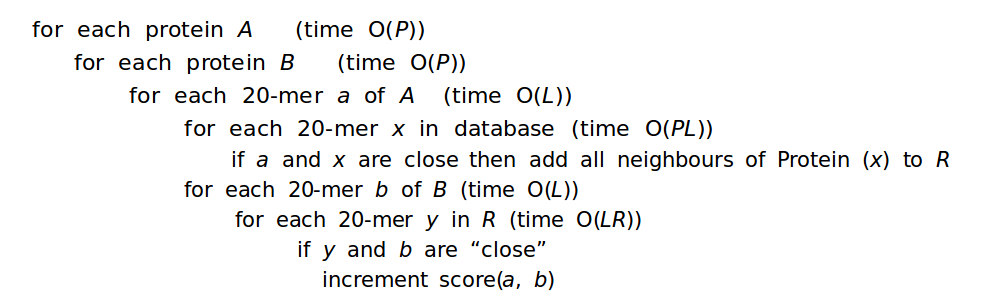
\includegraphics[width =17cm]{img/psedo_code_pipe.png}
\caption[The pseudocode of PIPE]{The pseudocode of PIPE.  \label{fig_pseudocode_pipe}}
\end{center}
\end{figure} 

The second version of PIPE, PIPE2 \cite{Pitre08_PIPE2}, increased both the speed and the accuracy from the previous version. 

For speed, instead of computing all similar pieces "on the fly", PIPE2 pre-computes all similar pieces for all protein sequences and stores them locally. PIPE2's pseudocode is shown in Figure \ref{fig_pseudocode_pipe2}. All pieces that are similar with $a$ and $b$ have been pre-computed so that the program does not waste time on computing the same re-occurring piece repeatedly. The time complexity of PIPE2, ignoring the pre-computating part, is improved to $O(P^2L^2R)$ where the size of $R$ is uncertain. After running PIPE2 for more than 80 hours, we estimated its running time on the entire human interactome prediction to be 1520 days.   
\begin{figure}[h!]
\begin{center}
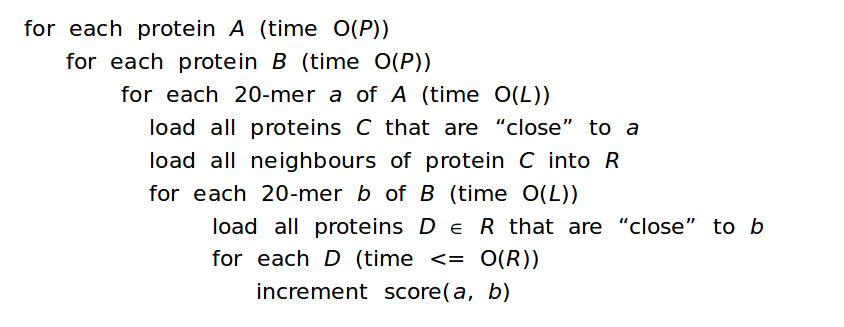
\includegraphics[width =15cm]{img/PIPE2_psedu.png}
\caption[The pseudocode of PIPE2]{The pseudocode of PIPE2.  \label{fig_pseudocode_pipe2}}
\end{center}
\end{figure} 

In terms of accuracy improvement, PIPE2 applies a binary filter which works as shown in Figure \ref{fig_binary_filter}. The binary filter flattens the matrix by checking the surrounding areas. For each cell containing the value $c$, if the surrounding eight cells have more non-zero values than zero values, then it replaces $c$ with 1, otherwise it replaces $c$ with 0. For example, the middle cell 34, has three non-zero values and five zero-values around it, so the filter replaces 34 with 0.

\begin{figure}[h!]
\begin{center}
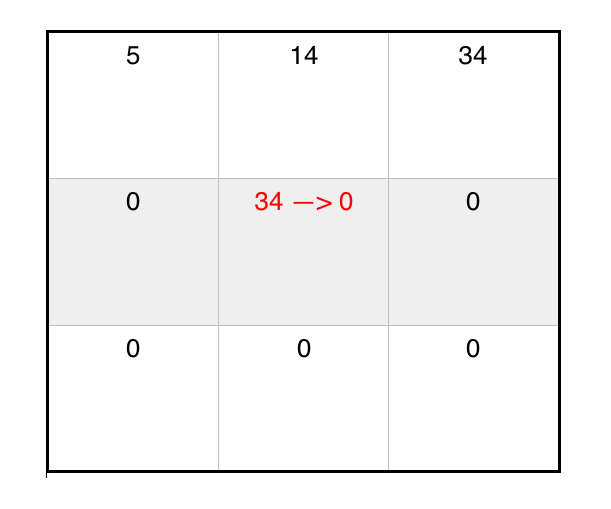
\includegraphics[height = 4 cm]{img/binary_filter.png}
\caption[The binary filter of PIPE2]{The binary filter of PIPE2. The centered number is replaced with 1 if there are more non-zero values than zero values in the surrounding eight cells, with 0 otherwise. From \cite{Pitre08_PIPE2}. \label{fig_binary_filter}}
\end{center}
\end{figure} 

PIPE's third version \cite{schoenrock2011mp}, PIPE3, parallels PIPE2. The algorithm is still slow, but it was the first program able to predict the entire human interactome. It took over 3 months to run the entire human proteome on 50 nodes with 12,800 parallel computational threads.

\subsubsection{Martin's Program}
Martin \cite{Martin05_PPIpred} is one of the earliest PPI perdition methods that use machine learning. It is highly cited and still considered one of the most effective ones. The workflow of Martin is shown in Figure \ref{fig_Martin}. The core idea of this method is using Support Vector Machine (SVM) \cite{hearst1998support} to classify PPIs. The inputs to the SVM is the encoding of two protein sequences. Encoding protein sequences were not a well studied problem at that time, and their solution was to use signature molecular descriptor \cite{visco2002developing, faulon2003signature1, faulon2003signature2}. The signature of a sequence $A$ is defined as $s(A) = \sigma_iz_i$ where $z_i$ is the all trimers of amino acids and $\sigma_i$ is the number of occurrences of trimer $z_i$. Each trimer put the centered residue at front and the two neighboring residues afterwards. For example, the signature of the sequence $LVMTTM$ is denoted as $s(LVMTTM) = V(LM)+M(TV)+2T(MT)$. The two signatures are further converted into two tensors and then computed the tensor product.
\begin{figure}[h!]
\begin{center}
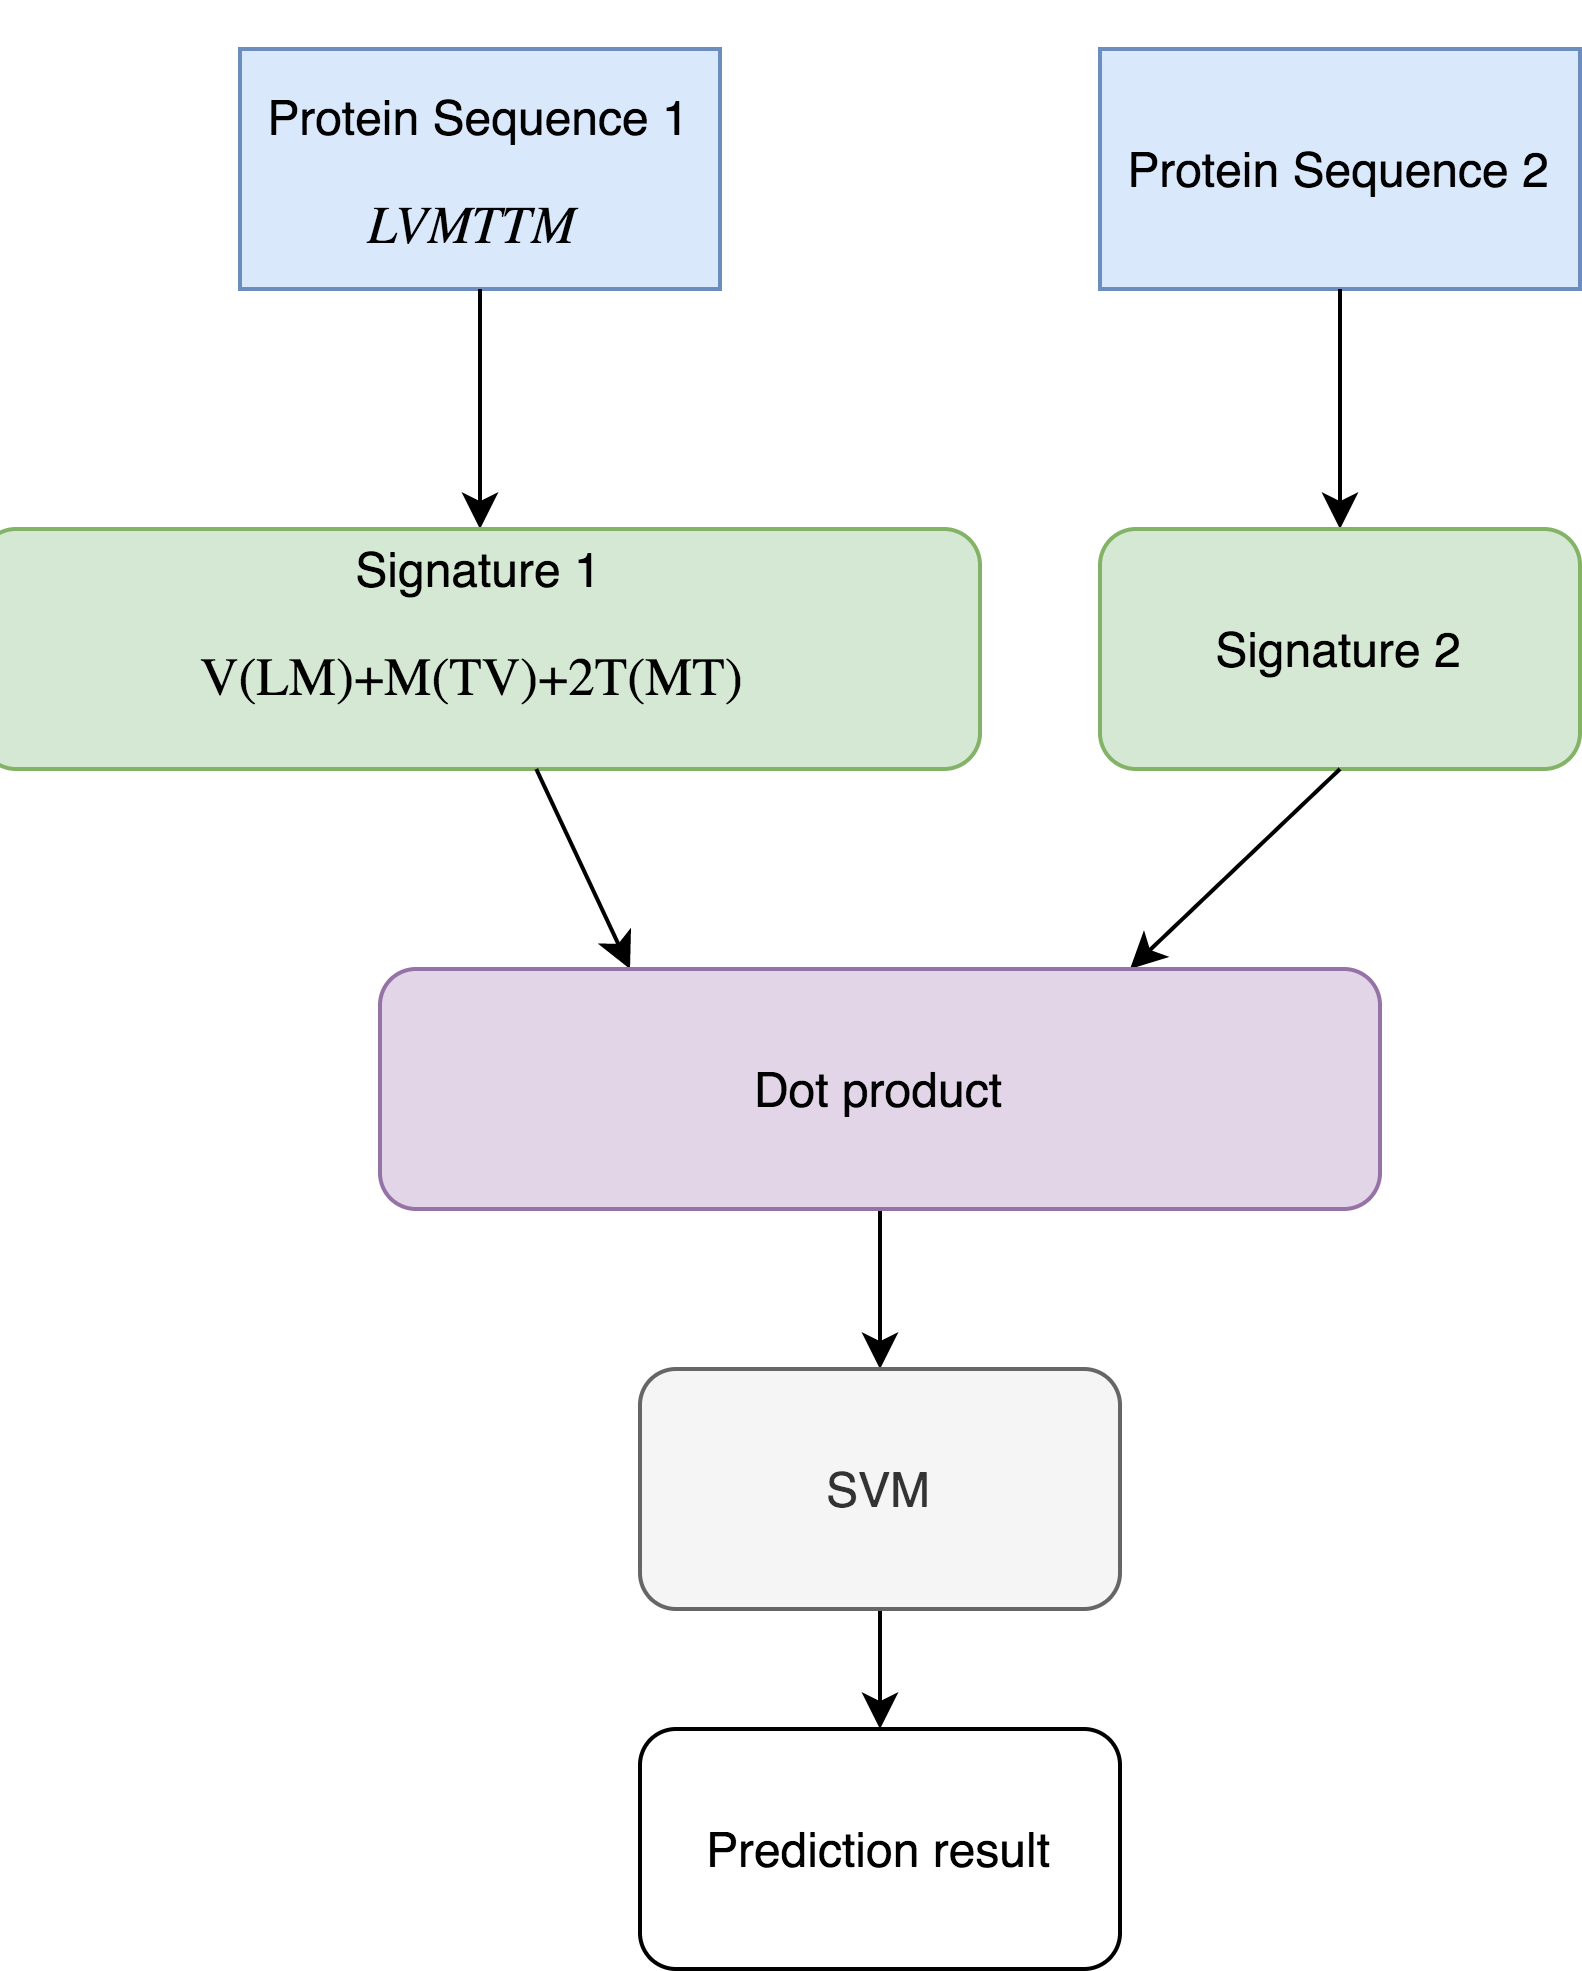
\includegraphics[height =7 cm]{img/sigProd.png}
\caption[The workflow of Martin]{The workflow of Martin. Two input protein sequences are encoded into signatures. The dot product of the two signatures are then computed. SVM is used to classify the dot product into interaction and non-interaction.  \label{fig_Martin}}
\end{center}
\end{figure} 

\subsubsection{Shen's Program}
Shen et al. \cite{Shen07_PPIpred} proposed a sequenced-based PPI prediction method. This method uses also machine learning techniques to make predictions. Their program uses protein sequences and PPIs as training data. Then it classifies new pairs of proteins with support vector machines (SVM) and a kernel function.

SVMs are used for classifying PPIs into two different sets, interacting or non-interacting. The kernel function is used for mapping training data into a higher dimension, in order to classify it linearly. A detailed introduction about SVM and kernel function can be found for instance in \cite{trevor2001elements}.

A key point in machine learning is how to "learn" more useful information from training data. Shen et al. first represent amino acids by vectors (see Figure \ref{fig:shen}). Every three amino acids are grouped as a vector space $(V, F)$, where $V$ is the encoded value, from 1 to 343, and $F$ is the frequency with which those three amino acids appear. For example, the first three amino acids are encoded as (342, 1), because this combination has only appeared once. The 20 amino acids are classified into 7 classes based on the dipoles and volumes of side chain. A detailed classification is shown in Figure \ref{fig:shen_clas}.
\begin{figure}[h!]
\begin{center}
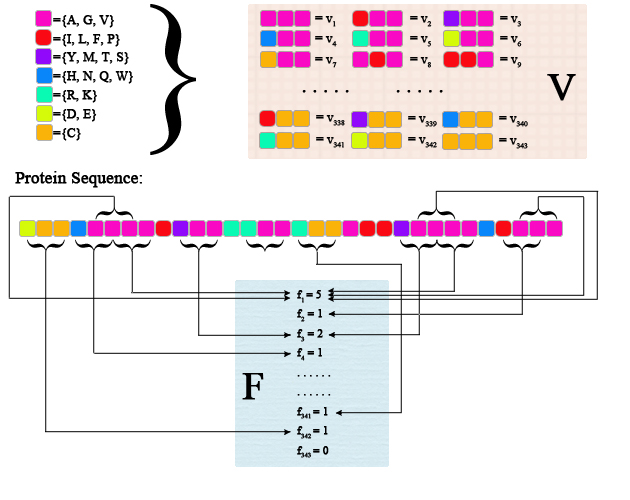
\includegraphics[height =13 cm, width = 13cm]{img/C_3_encode.jpg}
\caption{Constructing the vector space (V, F) of a protein sequence. From: \cite{Shen07_PPIpred} \label{fig:shen}}
\end{center}
\end{figure}

\begin{figure}[h!]
\begin{center}
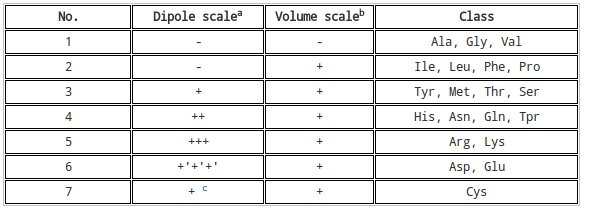
\includegraphics[height =5 cm, width = 8cm]{img/shen_clas.jpeg}
\caption{Classification of amino acids. From: \cite{Shen07_PPIpred} \label{fig:shen_clas}}
\end{center}
\end{figure}

\subsubsection{Guo's Program}
Guo et al. \cite{Guo08_PPIpred} proposed another PPI prediction approach.
This method uses SVMs and auto covariance (AC) to make predictions.

Similarly with the methods mentioned in 2.5.1 and 2.5.3, SVMs are used for classifying new pairs of proteins into interacting or non-interacting sets. Each amino acid in a protein sequence is represented as neighbouring effects and physicochemical properties (shown in Figure \ref{fig:guo_ac}). According to their optimization experiment, for each amino acid, they take into account 30 neighbour amino acids of it. This neighbouring effect is then translated into a numerical value. The physicochemical properties of each amino acids are shown in Figure \ref{fig:guo_ph_ch} where H1 = hydrophobicity, H2 = hydrophilicity, V = volume of side chains, P1 = polarity, P2 = polarizability, SASA = solvent accessible surface area, NCI = net charge index of side chains. Variables of neighbouring effect and physicochemical properties be will used to calculate AC variables. SVM will take these AC variables as input to make predictions.
\begin{figure}[h!]
\begin{center}
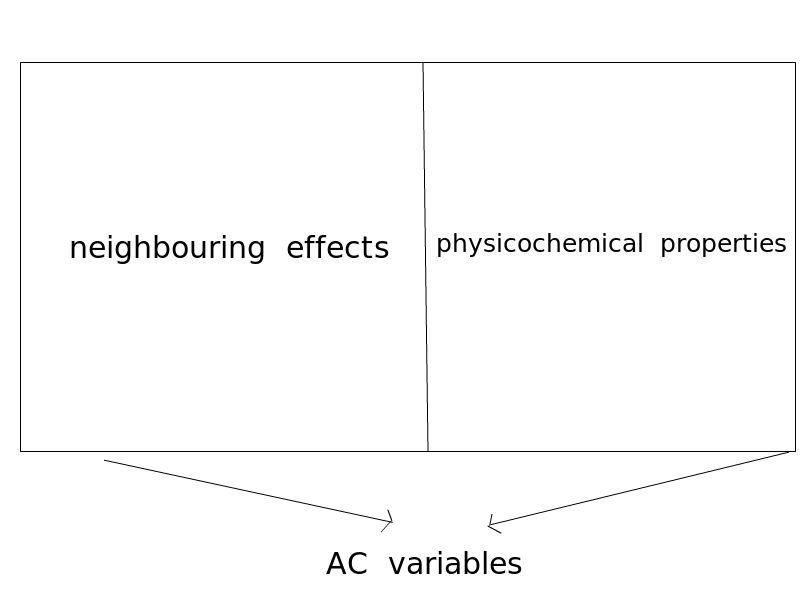
\includegraphics[height =6 cm, width = 8cm]{img/guo_ac.jpg}
\caption{Representation of each amino acid\label{fig:guo_ac}}
\end{center}
\end{figure}

\begin{figure}[h!]
\begin{center}
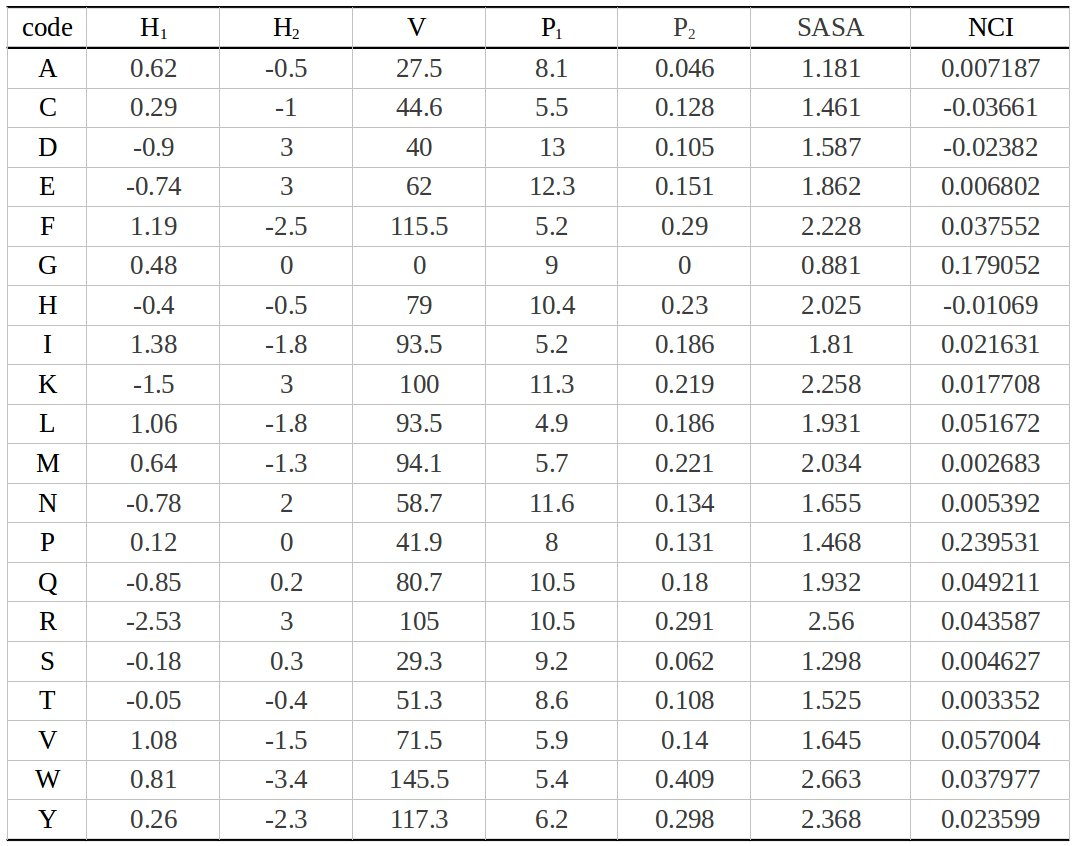
\includegraphics[height =12 cm, width = 12cm]{img/guo_ph_che.jpeg}
\caption{Values of the seven physicochemical properties for each amino acid. From \cite{Guo08_PPIpred} \label{fig:guo_ph_ch}}
\end{center}
\end{figure}

\subsubsection{Ding's Program}
Ding et al. \cite{ding2016predicting} published a program utilizing random forest classifier for PPI prediction. The flowchart of the program is shown in Figure \ref{fig_Ding}. The protein sequences are encoded into a 638-D matrix consisting k-gram embedding and electrostatic and hydrophobic properties.
\begin{figure}[h!]
\begin{center}
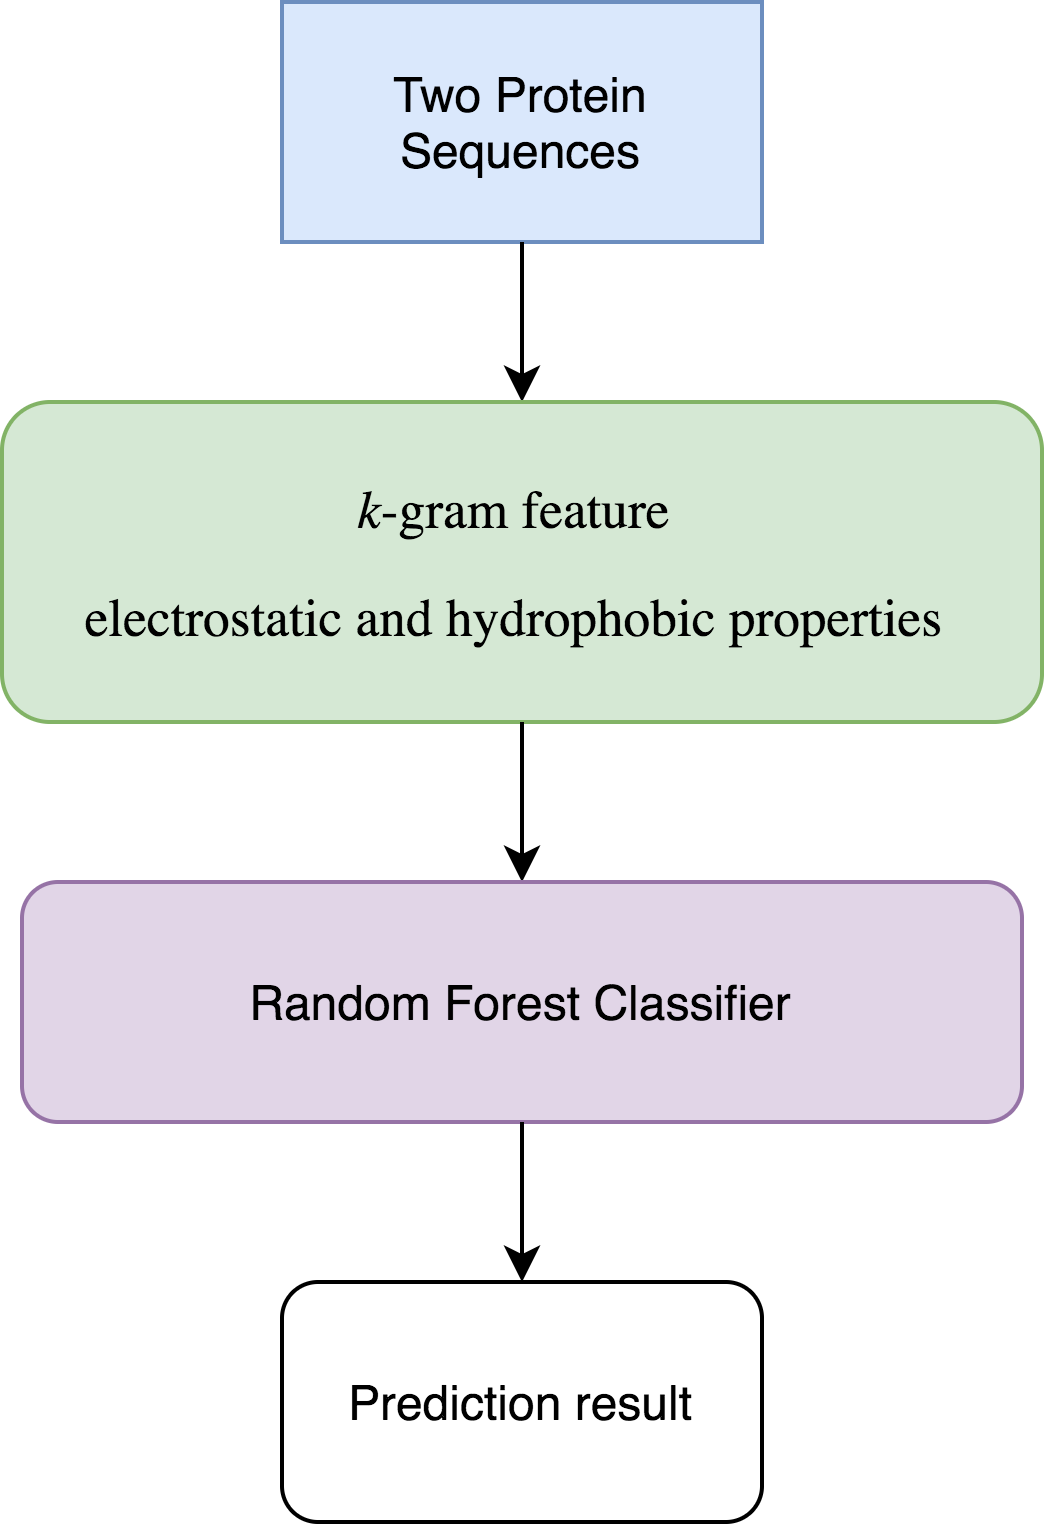
\includegraphics[height =7 cm]{img/Ding.png}
\caption[The workflow of Ding's program]{The workflow of Ding's program. The two input protein sequences are represented using a vector of dimension 638, consisting k-gram embedding and electrostatic and hydrophobic properties. The classifier is random forest. \label{fig_Ding}}
\end{center}
\end{figure} 
% \subsubsection{DPPI}
% DPPI \cite{hashemifar2018predicting} is a recent PPI prediction program using deep learning. It employs a Siamese-like network structure which learns from two proteins. The input sequences are firstly represented using PSSMs, then both matrices are passed to convolutional layers. Then a random projection module is applied to reduce the dimension of the tensor as well as to improve the prediction performance. In the end a linear layer outputs the prediction result.
% \begin{figure}[h!]
% \begin{center}
% 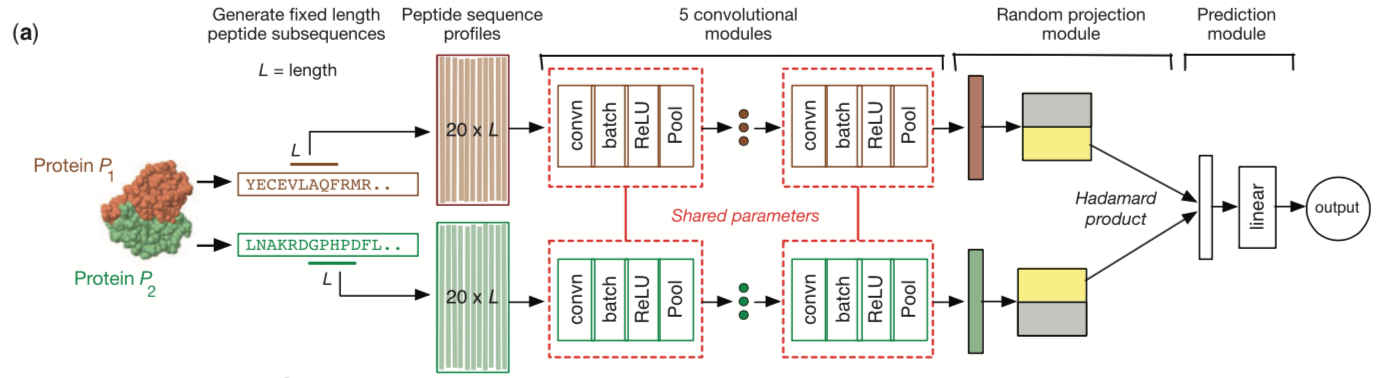
\includegraphics[height =6 cm, width = 17cm]{img/DPPI.png}
% \caption[The architecture of DPPI]{The architecture of DPPI. The sequences are encoded using PSSMs, passed into convolutional random projection, and linear layers. From \cite{hashemifar2018predicting} \label{fig_DPPI}}
% \end{center}
% \end{figure} 
% \subsubsection{PIPR}
% PIPR \cite{chen2019multifaceted} is one of the most recent PPI predictors. Similar to DPPI, it also employees a Siamese-like network using deep learning algorithms. As shown in Figure \ref{fig_PIPR}, two protein sequences are represented using embedding. The embedding contains two parts: Skip-Gram \cite{mikolov2013distributed} based embedding and electrostaticity and hydrophobicity characteristics. The embedding is then passed to residual RCNN network. The residual CRNN consists convolutional and bidirectional GRU layer. The GRU layer has shortcut connection between the input and the output. The outputs of the RCNN unit is put together using element-wise multiplication, and then the product is passed to fully-connected layers for prediction. 

% \begin{figure}[h!]
% \centering
% \begin{subfigure}[b]{\textwidth}
%   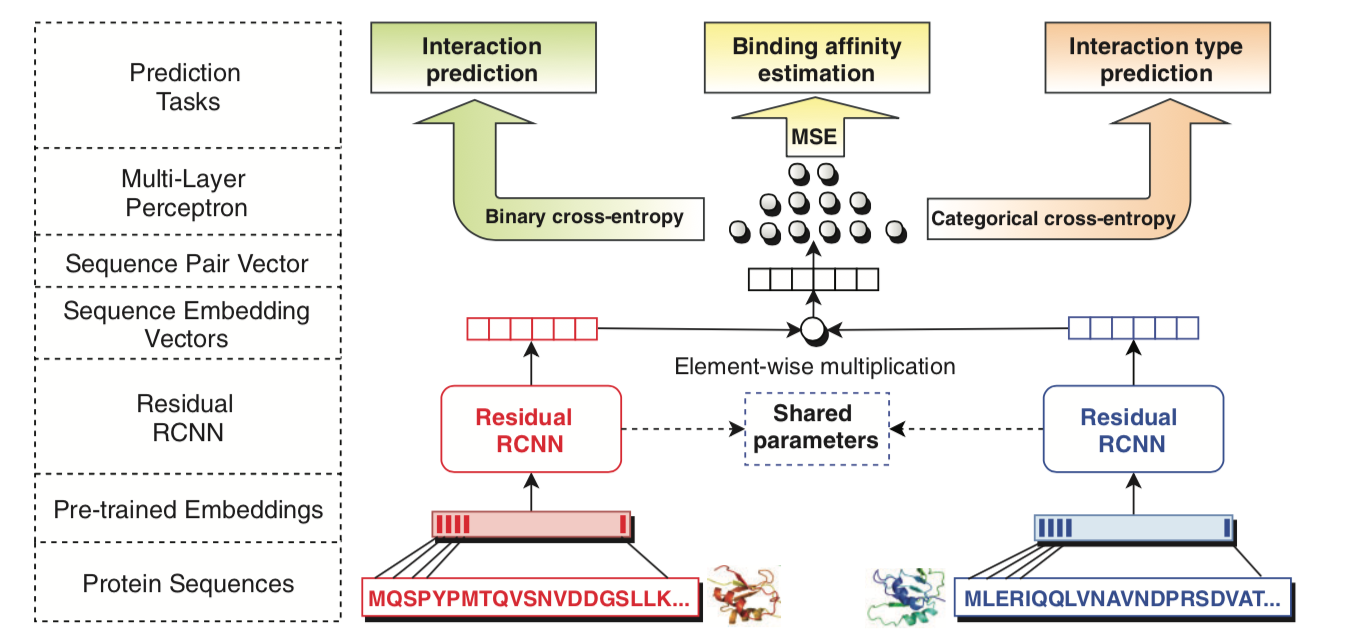
\includegraphics[width = 17cm]{img/PIPR_archi.png}
%   \caption{}
%   \label{fig_Ng1} 
% \end{subfigure}

% \begin{subfigure}[b]{\textwidth}
%   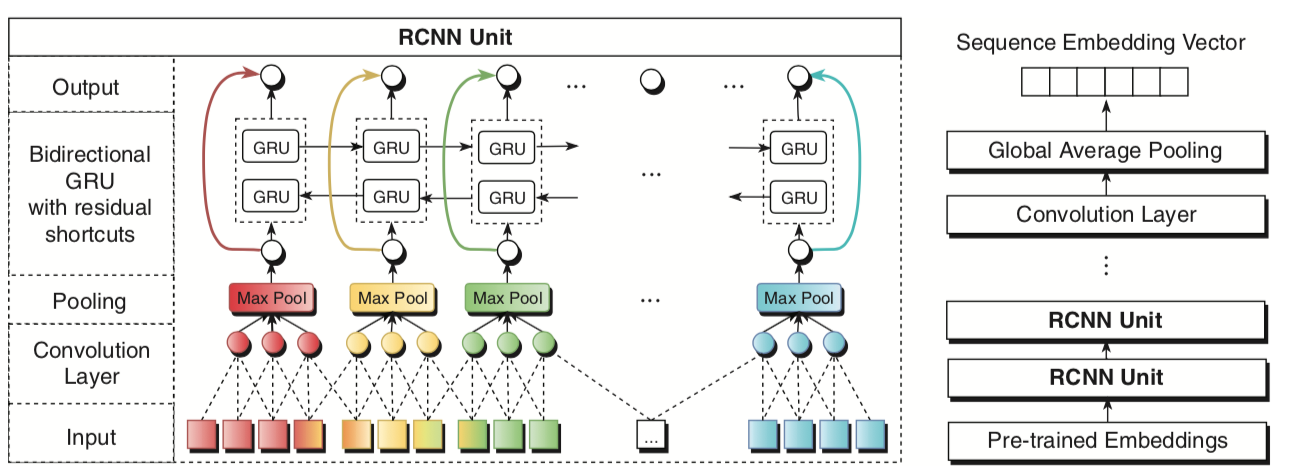
\includegraphics[width = 17cm]{img/PIPR.png}
%   \caption{}
%   \label{fig_PIPR}
% \end{subfigure}

% \caption[The architecture of PIPR]{(a) The overall architecture of PIPR. The flowchart consists input sequences, embedding, residual RCNN, element-wise multiplication, multi-layer perceptron. (b) The details of the RCNN unit. The RCNN combines a CNN and a RNN components. The RNN part is bidirectional GRU layer with residual shortcuts that bridge the input and the output of the GRU layer.}
% \end{figure}

\section{Methods}
We describe in this section both the algorithm and the implementation of SPRINT in details.
\subsection{Basic Idea}
Proteins similar with interacting proteins are likely to interact as well. That is, if $P_1$ is known to interact with $P_2$ and the sequences of $P_1$ and $P'_1$ are highly similar and the sequences of $P_2$ and $P'_2$ are highly similar, then $P'_1$ and $P'_2$ are likely to interact as well. In a way or another, this is essentially the idea behind the brute force calculation of PIPE as well as the machine learning algorithms of Martin, Shen, and Guo. 

SPRINT uses a complex algorithm to quickly evaluate the contribution of similar subsequences to the likelihood of interaction. SPRINT has two main steps: computing HSP and predicting interactions. 

High-scoring segment pairs (HSPs) are similar subsequences among all input sequences. SPRINT first detects these HSPs from the input protein sequences. Figure \ref{fig_compute_hsp} is the visualization of the process. Four proteins, P1 to P4, are input to the Compute HSPs program. After computation, three HSP pairs are found, that is  subsequences A1, B1, C1 are similar to A2, B2, C2 respectively.  

\begin{figure}
  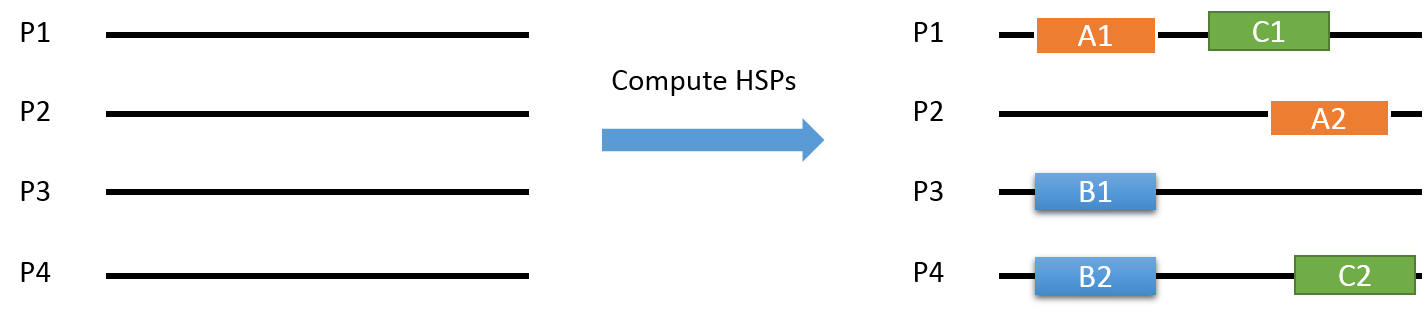
\includegraphics[width=0.95\textwidth]{img/compute_hsp}
\caption[The idea of computing HSPs]{The idea of computing HSPs. P1 - P4 represent four protein sequences. (A1, A2), (B1, B2), (C1, C2) represent three pairs of HSPs. Blocks with the same colour indicate a pair of HSP.}
\label{fig_compute_hsp}  
\end{figure}

After computing the HSPs, SPRINT takes in both the similarities and known PPIs as inputs and predict interactions. The idea of predicting interactions in SPRINT is shown in Figure \ref{fig_predict_PPI}. A, B, and C are HSP segments, and P1-3 and Q1-3 are proteins. Known PPIs (P1, Q1) and (P2, Q2) are fed to SPRINT along with the HSPs they contain. SPRINT assumes that in an known interaction, all HSPs are possible binding sites that cause the interaction. For example, (A, B) and (A, C) are assumed to be the binding sites in the interactions (P1, Q1) and (P2, Q2) repetitively, and they are expected to behave the same in an novel interaction (P3, Q3). Thus, the interaction score of (P3, Q3) is increased based on the possible biding between (A, B) and (A, C). The higher the score, the more confidently SPRINT claims the interaction. 

\begin{figure}
  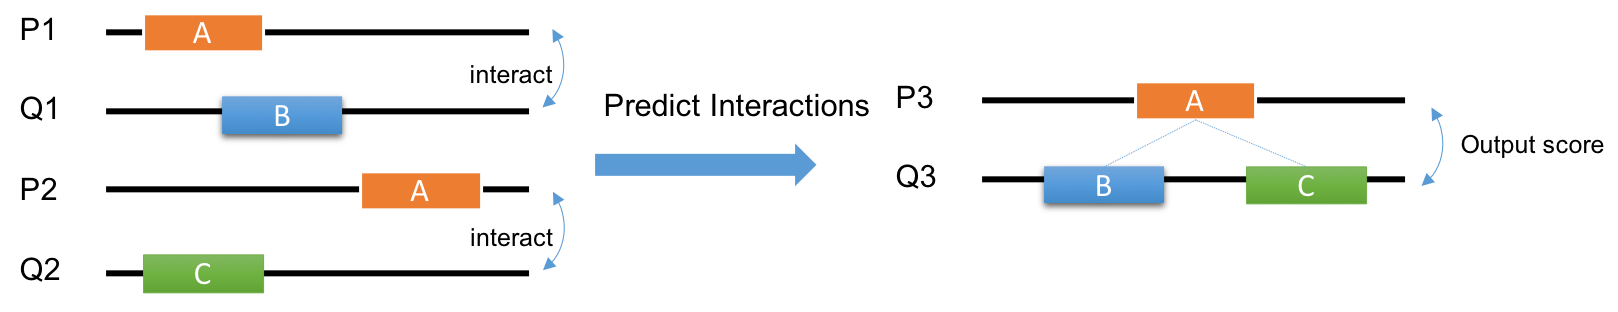
\includegraphics[width=0.95\textwidth]{img/predict_PPI.png}
\caption[The idea of predicting PPIs]{The idea of predicting PPIs. A, B, C are HSPs. The blocks with the same colour indicate HSP pairs. (P1, Q1) and (P2, Q2) are known interactions. The interaction score of (P3, Q3) is calculated.}
\label{fig_predict_PPI}  
\end{figure}

% \begin{figure}[h!]
% \centering
% 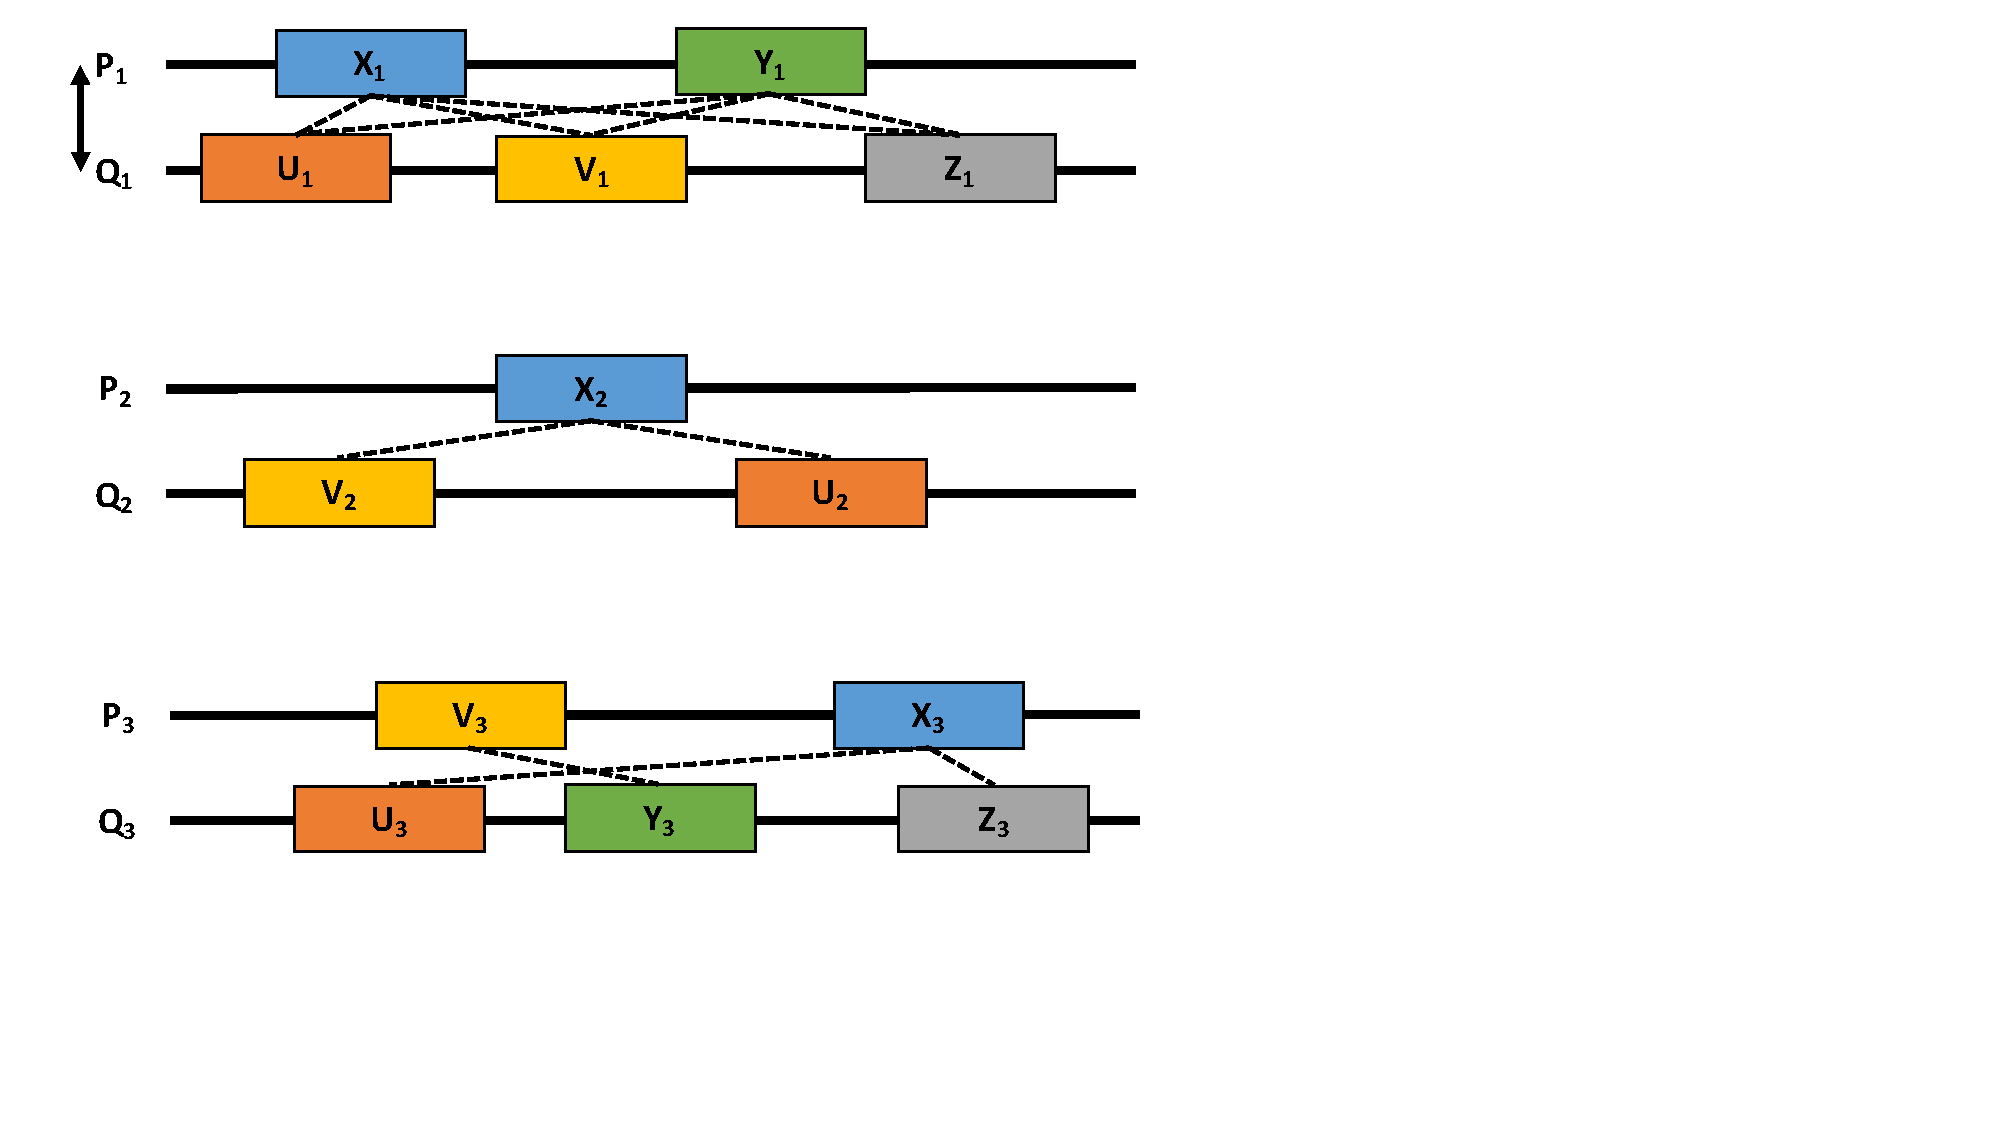
\includegraphics[width=8cm]{img/fig_idea.pdf}
% \caption[Interaction inference]{Interaction inference. The proteins $P_1$ and $Q_1$ are known to interact; blocks of the same colour represent occurrences of similar subsequences. Dashed lines indicate potential contributions to interactions: there are six between $P_1$ and $Q_1$ and they imply two between $P_2$ and $Q_2$ and three between $P_3$ and $Q_3$. \label{fig_idea}}
% \end{figure}

Long similar regions should have a higher weight than short ones. To account for this we assume that all contributing blocks have a fixed length $k$ %(default $k = 20$) 
and that a region of length $\ell$ contributes $\ell-k+1$ blocks. As $k$ is fixed, this grows linearly with $\ell$. The precise score is given later in this section.

We put together the workflow of SPRINT in Figure \ref{fig_SPRINT_workflow}, The details of each step are given in the following sections.

\begin{figure}[h!]
\centering
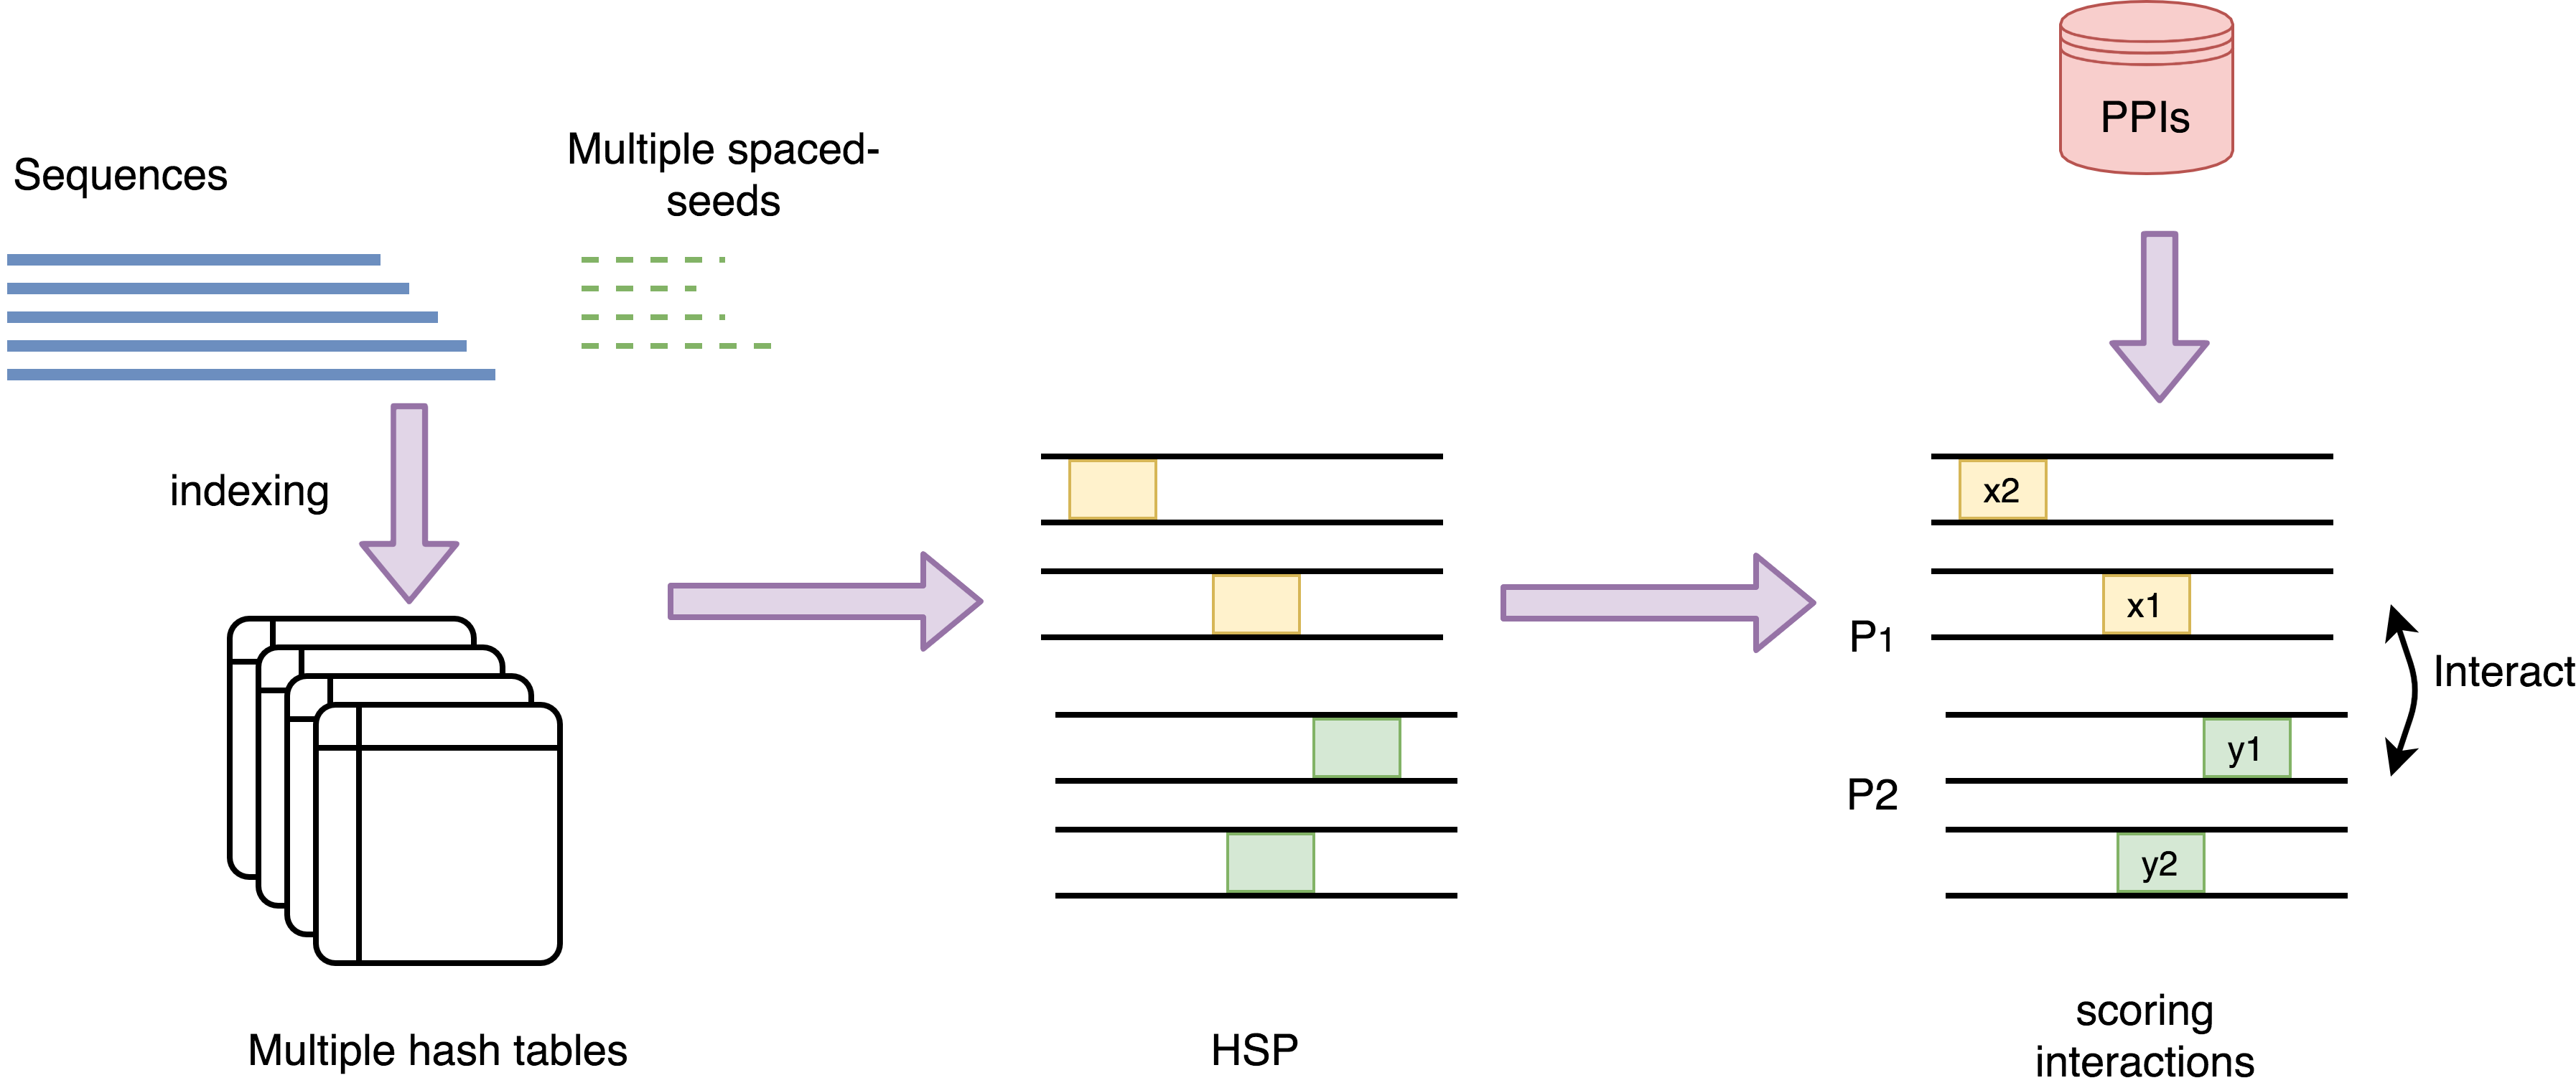
\includegraphics[width=15cm]{img/SPRINT_workflow.png}
\caption[The workflow of SPRINT]{The workflow of SPRINT. First sequences are indexed with spaced-seeds into multiple hashtables (left). Then HSPs are detected by fast traversing the hashtables (middle). Last, known PPIs are loaded and used together with HSPs for predicting new interactions. \label{fig_SPRINT_workflow}}
\end{figure}

\subsection{Detecting Similarities \label{sec_detect_simi}}
As mentioned above, the first step of SPRINT is the identification of similar subsequences among the input protein sequences. This is done using multiple spaced seeds with the hit-and-extension method.

A spaced match requires only the amino acids in positions corresponding to {\tt 1}'s in the seed to match. For example,  a hit in seed 11****11***1 only needs the amino acids in positions 1, 2, 7, 8, and 12 have to match. Given the spaced seed above, two \textit{exact} spaced matches are underlined in Figure~\ref{fig_s-match}(a).

\begin{figure}[h!] 
\centering
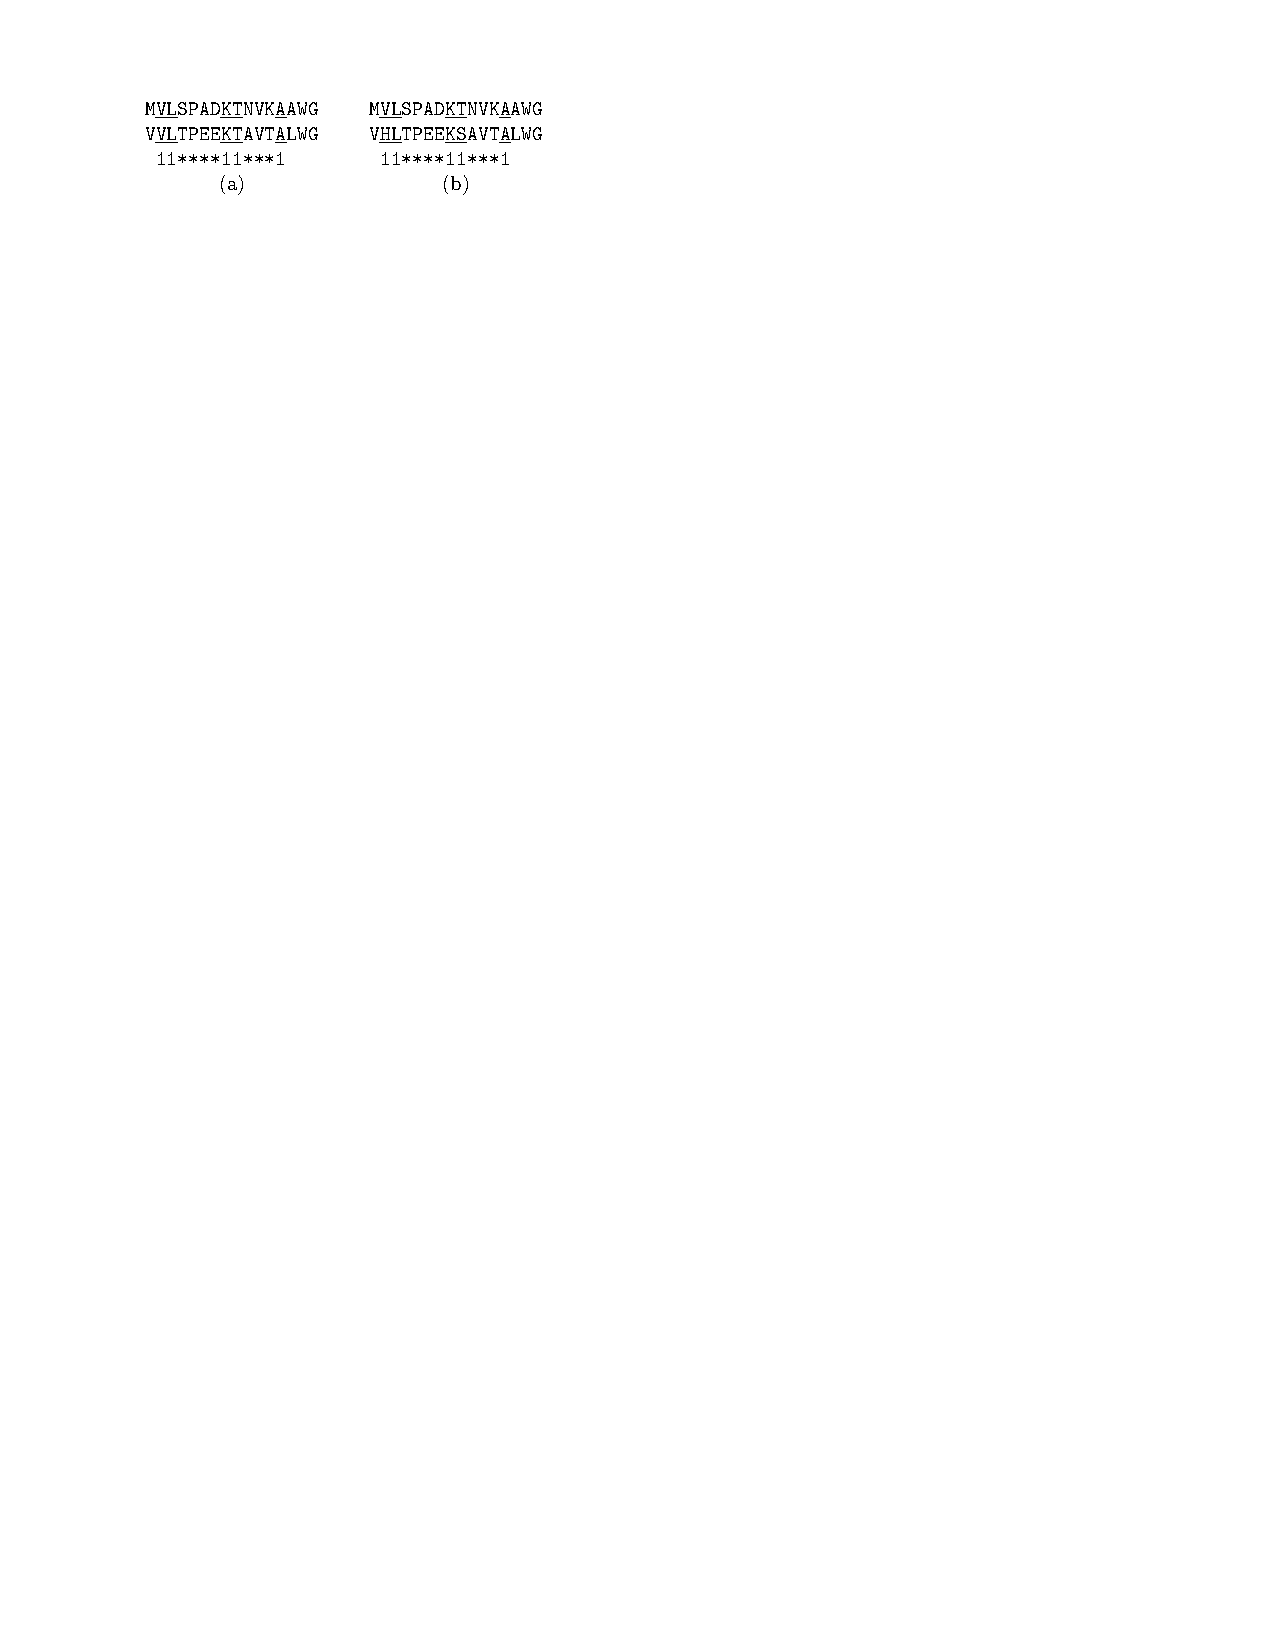
\includegraphics{img/fig_s-match.pdf}
\caption[Spaced-seed hits]{An exact hit (a) and an approximate hit (b) of the same spaced seed.\label{fig_s-match}}
\end{figure}

There is a trade-off between speed and sensitivity. Lower weight has increased sensitivity because it is easier to hit similar regions but lower speed since more random hits are expected and have to be processed. The best value for our problem turned out to be five.

As briefly mentioned in Section \ref{sec_multiple_spaced_seed}, the distribution of matches and don't care positions is crucial for the quality of the seeds and we have used SpEED~\cite{Ilie07_spacedSeeds,Ilie11_SpEED} to compute the following seeds used by SPRINT; we have experimentally determined that four seeds of weight five are the best choice: $\textsc{Seed}_{4,5} = \{$\texttt{11****11***1}, \texttt{1**1*1***1*1}, \texttt{11**1***1**1}, \texttt{1*1******111}$\}$.

In order to further increase the probability of finding similar subsequences, we consider also hits between similar matches, as opposed to exact ones. For example, the two amino acid sequences in Figure~\ref{fig_s-match}(b), though similar, do not have any \textit{exact} spaced matches. In order to capture such similarities, we consider also hits consisting of \textit{similar} spaced matches; an example is shown by the underlined subsequences in Figure~\ref{fig_s-match}(b).

To make this idea precise, we need a few definitions. {\it Spaced-mers} are defined analogously with $k$-mers but using a spaced seed. A $k$-mer is a contiguous sequence of $k$ amino acids. Given a spaced seed, a spaced-mer consists of $k$ amino acids interspersed with spaces, according to the seed. For a spaced seed $s$, we shall call the spaced-mers also $s$-mers. Figure~\ref{fig_s-mers} shows an example of all $s$-mers of a sequence, for $s=${\tt 11****11***1}:

\begin{figure}[h!]
\centering
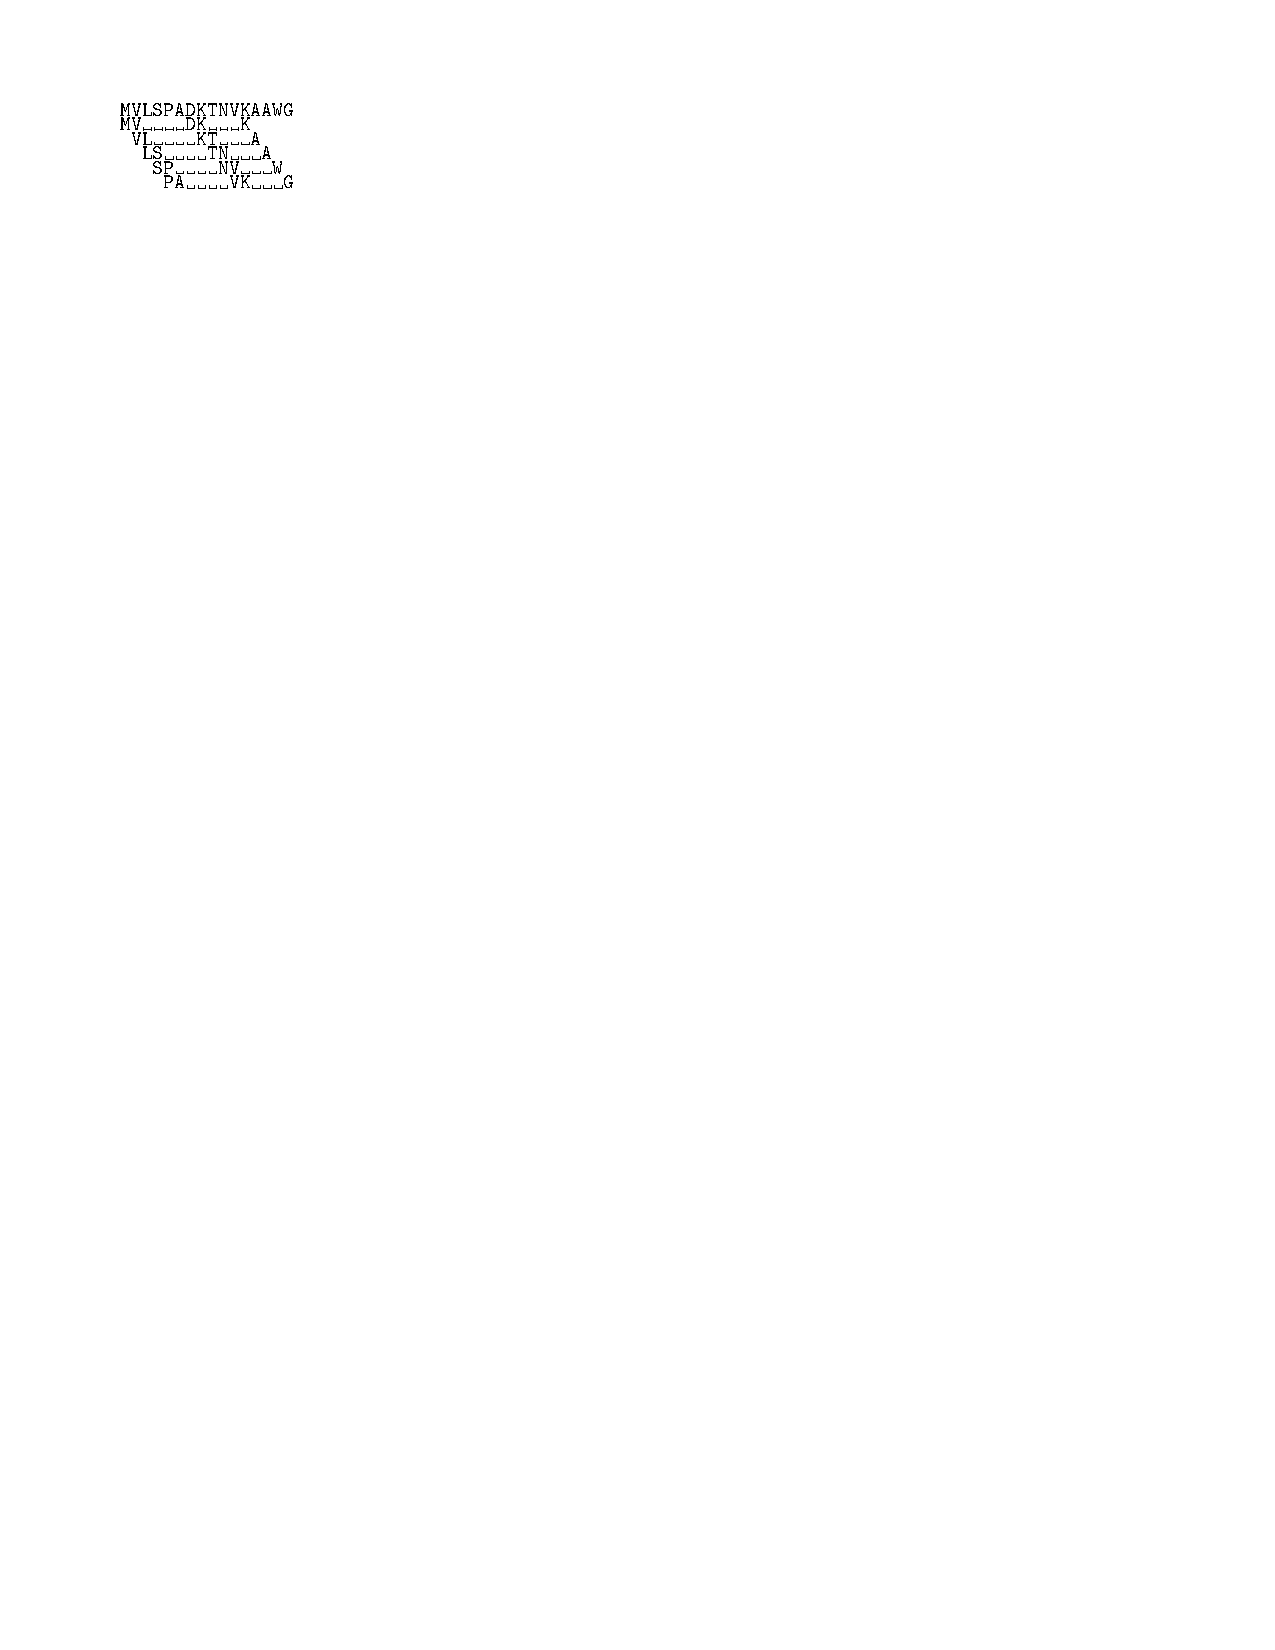
\includegraphics{img/fig_s-mers.pdf}
\caption{An example of all $s$-mers of a sequence.\label{fig_s-mers}}
\end{figure}

An exact hit therefore consists of two occurrences of the same $s$-mer. An approximate hit, on the other hand, requires two similar $s$-mers.
Assume a similarity matrix $M$ is given. Given a seed $s$ and two $s$-mers $w$ and $z$, the score between the two $s$-mers is given by the sum of the scores of the pairs of amino acids in the two $s$-mers, that is, we sum over indexes corresponding to \texttt{1}'s in the seed:
\begin{equation}\label{eq:s-mer_score}
S_\textrm{$s$-mer}(w,z) = \sum_{s[i]=\texttt{1}}M(w_i,z_i)\ .
\end{equation}
For example, for the $s$-mers $w = \texttt{VL\textvisiblespace\textvisiblespace\textvisiblespace\textvisiblespace KT\textvisiblespace\textvisiblespace\textvisiblespace A}$ and $z = \texttt{HL\textvisiblespace\textvisiblespace\textvisiblespace\textvisiblespace KS\textvisiblespace\textvisiblespace\textvisiblespace A}$ from Figure~\ref{fig_s-match}(b), we have $S_\textrm{$s$-mer}(w,z) = M(\texttt{V},\texttt{H}) + M(\texttt{L},\texttt{L}) + M(\texttt{K},\texttt{K}) + M(\texttt{T},\texttt{S}) + M(\texttt{A},\texttt{A}).$

Using (\ref{eq:s-mer_score}), we define the set of $s$-mers that are \textit{similar} with a given $s$-mer $w$:
\begin{equation}\label{eq:Sim}
\textrm{Sim}(w) = \{z \mid z \text{ $s$-mer}, S_\textrm{$s$-mer}(w,z) \ge \Thit\}\ .
\end{equation}

Note that $\textrm{Sim}(w)$ depends on the parameter $\Thit$ that controls how similar two $s$-mers have to be in order to form a hit. It also depends on the seed $s$ and the similarity matrix $M$ but we do not include them into the notation, for clarity.

All such hits dues to similar $s$-mers are found and then extended both ways in order to identify similar regions. That means, now we have to evaluate the similarity of all the amino acids involved, so we use the regular $k$-mers.
The score between two $k$-mers $A$ and $B$ is computed as the sum of all scores of corresponding amino acids:
\begin{equation}\label{eq_score_kmer}
S_\textrm{$k$-mer}(A,B) = \sum_{i=1}^kM(A_i,B_i)\ ,
\end{equation}
where $A_i$ is the $i$th amino acid of $A$. Given a hit that consists of two $s$-mers $w$ and $z$, we consider the two $k$-mers that contain the occurrences of the two $s$-mers $w$ and $z$ in the center, denoted $\textrm{$k$-mer}(w)$ and $\textrm{$k$-mer}(z)$. If $S_\textrm{$k$-mer}(\textrm{$k$-mer}(w),\textrm{$k$-mer}(z)) \ge \Tsim$, then the two regions are deemed similar. Note the parameter $\Tsim$ that controls, together with $k$-mer size $k$, how similar two regions should be in order to be identified as such.

Details of the fast implementation are given next. The protein sequences are encoded into bits using five bits per amino acid. We encode each amino acid with 5 bits. Blocks of 5 bits can have $2^5$ = 32 different values. So 5 bits are more than enough for encoding twenty amino acids. 
Table \ref{tab_A_A_encoding} shows in detail the encoding of each amino acid. The five bits used for encoding are unrelated with the weight of the spaced seeds employed. It is a coincidence that both numbers are five. Each protein sequence is encoded as an array of unsigned 64-bit integers; each 64-bit integer stores 12 amino acids within 60 bits and 4 bits are unused. Each spaced seed is encoded using also five bits per position, {\tt 11111} for a {\tt 1} (match) and {\tt 00000} for a {\tt *} (don't care), also into an unsigned 64 integer.  

\begin{table}[h!]
\begin{center}
\begin{tabular}[h!]{|c|c|c|} 
%c stands for centre, l for left, r for right; the | puts lines in between, and the hline puts a horizontal line in
\hline
Amino acid name & Notation in FASTA format & 5-bit encoding \\
\hline
Alanine & A & 00000 \\
\hline
Arginine & R & 00001\\
\hline
Asparagine & N & 00010 \\
\hline
Aspartic acid & D & 00011 \\
\hline
Cysteine & C & 00100 \\
\hline
Glutamine & Q & 00101 \\
\hline
Glutamic acid & E & 00110 \\
\hline
Glycine & G & 00111 \\
\hline
Histidine & H & 01000\\
\hline
Isoleucine & I & 01001 \\
\hline
Leucine & L & 01010 \\
\hline
Lysine & K & 01011 \\
\hline
Methionine & M & 01100 \\
\hline
Phenylalanine & F & 01101 \\
\hline
Proline & P & 01110\\
\hline
Serine & S & 01111 \\
\hline
Threonine & T & 10000 \\
\hline
Tryptophan & W & 10001 \\
\hline
Tyrosine & Y & 10010 \\
\hline
Valine & V & 10011 \\
\hline
\end{tabular}
\caption[Amino acid encoding]{Amino acid encoding. Each amino is encoded with 5-bits (last column). \label{tab_A_A_encoding}}
\end{center}
\end{table}

All spaced-mers in all protein sequences are computed and stored in a hash table, together with their location in the protein sequences. Because of our representation, the computation of each spaced-mer requires only one bitwise AND and one bit SHIFT operation which is much faster than string operations. 

Finding HSPs start with finding hits, that is, matching $s$-mers. In order to do this fast, we use a hash table. All extracted $s$-mer will be stored in the hash table. For each seed, we have one hash table. The hash function is shown in \ref{eq_hash_func}. Liner probe is used for hash collision.  
\begin{equation}
entry\_index = s\_mer\_value \text{ }\%\text{ } hash\_size
\label{eq_hash_func}
\end{equation}

where the hash size is determined when encoding proteins. For each seed, the maximum number of $s$-mers is:
\begin{displaymath}
number{\_}of{\_}smers = \sum_{i=1}^{num\_of\_pro} (protein\_length - seed\_length +1).
\end{displaymath}

The program automatically chooses the smallest prime number which is bigger than the number of $s$-mers, from a list of precomputed large prime numbers, as hash size. Hash collisions are solved using linear probing. In each entry of the hash table, we store its $s$-mer value along with a pointer to an array of positions, which keeps a record of protein ids and starting positions of that $s$-mer. The pseudocode for computing the eight hash tables is given in Algorithm  \ref{algo:comp_ht}. Algorithm \ref{algo:insert_ht} shows the insertion into hash table in detail.

\begin{algorithm}[h!]
 \SetAlgoLined 
 \SetKwInOut{Input}{input}
\SetKwInOut{Output}{output}
\caption{Algorithm for computing hash tables \label{algo:comp_ht}}
 \Input{encoded\_proteins $EP$, 8 encoded\_seeds $S$}
 \Output{8 hash tables $HT$}
 \For {each seed $s\in S$}
 {
 	- initialize $ht\in HT$\\
 	- \For {each protein $p\in EP$}
 	{
 		- $temp\_protein\_sequence$ = $p$\\
 		- \For {$position\in [0 , (pro\_length - seed\_length + 1)]$}
 		{
			- $s$-mer = $s$ \& $temp\_protein\_sequence$\\
			- $temp\_protein\_sequence$ shift one position\\
			- insert\_into\_hash\_table ($s$-mer, $position$, $ht$)
 		}
 	}
 }
\end{algorithm}

\begin{algorithm}[h!]
 \SetAlgoLined 
 \SetKwInOut{Input}{input}
\SetKwInOut{Output}{output}
\caption{Algorithm for inserting $s$-mer into hash table \label{algo:insert_ht}}
 \Input{$s$-mer, $s$-mer$\_position$, $hash\_table$}
 \Output{}
	position $p$ = $s$-mer \% $hash\_size$ \\
	\If {$hash\_table[p] == \emptyset$}
	{
		insert ($s$-mer, $s$-mer$\_position$) into $hash\_table$[$p$]\\
	}
	\ElseIf {$s$-mer $== hash\_table[p].s$-mer}
	{
		add ($s$-mer$\_position$) into $hash\_table$[$p$] as a linked list\\
	}
	\ElseIf {$s$-mer $\neq hash\_table[p].s$-mer}
	{
		insert\_$s$-mer\_into\_hashtable($s$-mer, $p$ + 1, $hash\_table$)\\
	}
\end{algorithm}

Once all spaced-mers are stored, for each spaced-mer in the hashtable, all similar spaced-mers are computed and then all hits between the spaced-mer and similar ones are investigated from the table and extended in search for similarities. 

\subsection{Predicting Interactions}
As previously showed in Figure \ref{fig_SPRINT_workflow}, after obtaining the HSPs, the next step is to predict interactions.
\subsubsection{Post-processing Similarities}
We first process the similar subsequences we computed in the previous phase to remove those appearing too many times as they are believed to be just repeats that occur very often in the protein sequences without any relevance for the interaction process. We explain the algorithm on the toy example below. For the protein sequence {\tt MVLSPADKTNVKAAWG}, assume we have found the similarities marked by lines in  Figure~\ref{fig_similarities}(a). For example, the top line means that {\tt MVLSP} was found to be similar with another subsequence somewhere else, the bottom line represents the same about the subsequence {\tt KTNVKAAW}, etc. 

\begin{figure}[h!]
\centering
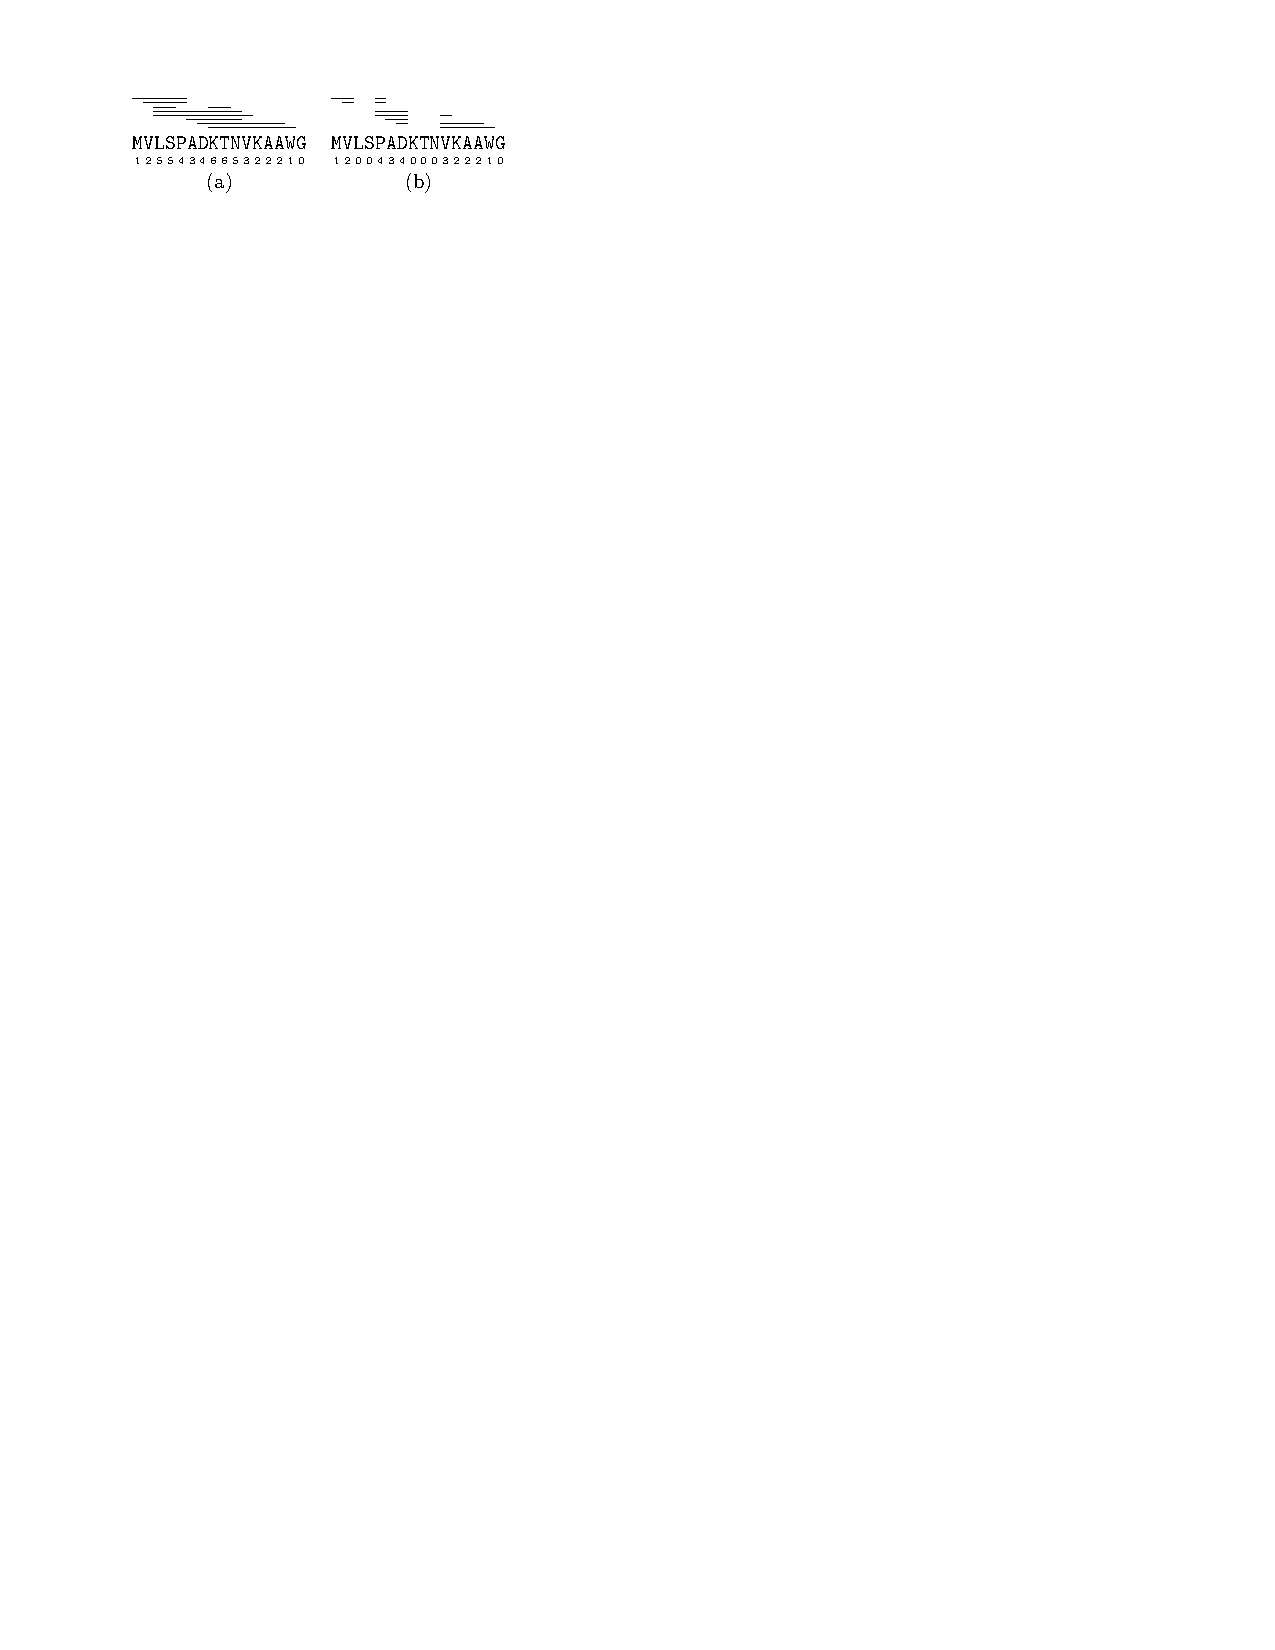
\includegraphics{img/fig_similarities.pdf}
\caption{An example of similarities before (a) and after (b) post-processing.\label{fig_similarities}}
\end{figure}

The counts in the bottom row indicate how many times each position occurs in all similarities found. (In the figure above, this means the number of lines that cover that position.) All positions with a high count, above a threshold $\Thc$, will be eliminated from all similarities, which will be modified accordingly. In our example, assuming the threshold is 5, positions 3, 4, 8, 9, and 10 have counts 5 or higher and are eliminated; see Figure~\ref{fig_similarities}(b). The new similarities are indicated by the lines above the sequence. For example, {\tt MVLSP} has positions 3 and 4 removed and becomes two similarities, {\tt MV} and {\tt P}. The counterpart of each similarity is modified the same way.
\subsubsection{Scoring Function}
What we have computed so far are HSPs, that is, pairs of similar subsequences of the same length. We now show how to score an interaction. First, we extend the definition of the score from $k$-mers to arbitrary subsequences of equal length. For two subsequences $X$ and $Y$ of length $n$, the score is given by the sum of the scores of all corresponding $k$-mer pairs; using \eqref{eq_score_kmer}:
\begin{equation}\label{eq_score_nmer}
S_e(X,Y) = \sum_{i=1}^{n-k+1}S_\textrm{$k$-mer}(X[i\pp i+k-1],Y[i\pp i+k-1])\ ,
\end{equation}
where $X[i\pp j] = X_iX_{i+1}\cdots X_j$. It is important to recall that any two similar sequences we find have the same length, therefore the above scoring function can be used.

Finally, we describe how the scores for whole protein sequences are computed. Initially all scores are set to zero. Each pair of proteins $(P_1, P_2)$ that are known to interact has its own contribution to the scores of other pairs. For each computed similarity $(X_1,Y_1)$ between $P_1$ and another protein $Q_1$ ($X_1$ is a subsequence of $P_1$ and $Y_1$ is a subsequence of $Q_1$) and for each similarity $(X_2,Y_2)$ between $P_2$ and another protein $Q_2$, the score between $Q_1$ and $Q_2$, $S_p(Q_1,Q_2)$, is increased, using \eqref{eq_score_nmer}, by:
\begin{equation}\label{eq_score_add}
\begin{array}{l}
S_p(Q_1,Q_2)\gets S_p(Q_1,Q_2)\\

 + \displaystyle{\frac{S_e(X_1,Y_1)(|X_2|-k+1)+ S_e(X_2,Y_2)(|X_1|-k+1)}{|Q_1||Q_2|}},
 \end{array}
\end{equation}
where $|Q|$ denotes the length of the amino acid sequence $Q$. That means, the score of each corresponding $k$-mer pair between $X_1$ and $Y_1$ is multiplied by the number of $k$-mers in $X_2$, that is, the number of times it is used to support the fact that $Q_1$ is interacting with $Q_2$. Similarly, the score of each corresponding $k$-mer pair between $X_2$ and $Y_2$ is multiplied by the number of $k$-mers in $X_1$. The score obtained this way is then normalized by dividing it by the product of the lengths of the proteins involved. 

Once the score are computed, by considering all given interactions and similar subsequences and computing their impact on the other scores as above, predicting interactions is simply done according to the scores. All protein pairs are sorted decreasingly by the scores; higher scores represent higher probability to interact. If a threshold is provided, then those pairs with scores above the threshold are reported as interacting. 

\subsection{Implementations}
\subsubsection{Tuneable Parameters}
\label{sec:parameter}
There are some tuneable parameters (see Table \ref{tab_parameter_SPRINT}) in SPRINT. In general, the default values are tuned experimentally and set based on the human datasets used in \cite{li2017sprint}, so it is recommended to use the default values if PPI prediction is performed on human datasets. The default values for the parameters are $k = 20$, $\Thit = 15$, $\Tsim = 35$, $M=PAM120$, and $\Thc = 40$. These values have been experimentally determined using only Park and Marcotte's data set. All the other datasets have been used exclusively for testing. The program is quite stable, the results being almost unaffected by small variations of these parameters.
\begin{table}[]
\begin{adjustwidth}{-2.5cm}{}
\caption{Tuneable Parameters in SPRINT}
\begin{tabular}{@{}lll@{}}
\toprule
Parameter & Default           & Description                                                        \\ \midrule
-Thit      & 15        & The similarity threshold to form a hit                             \\
-Tsim      & 35        & The similarity threshold to form an length-20 HSP                  \\
-M         & PAM120        & The scoring Matrix used to compute similarity between two subsequences \\
-Thc       & 40 & The threshold to consider a position high count                    \\ \bottomrule
\end{tabular}
\label{tab_parameter_SPRINT}
\end{adjustwidth}
\end{table}

\subsubsection{Pseudocode}
We put all the above together to summarize the SPRINT algorithm for predicting PPIs.
The input consists of the proteins sequences and PPIs. The default set of seeds is given by $\textsc{Seed}_{4,5}$ above but any set can be used.


\smallskip

\noindent
\setcounter{algccc}{0}
\underline{$\text{\sc SPRINT}(P_s,P_i)$}\\
\textbf{input:} protein sequences $P_s$, protein interactions $P_i$\\
\textbf{global:} seed set $\textsc{Seed}$\\
\textbf{output:} all protein pairs sorted decreasingly by score\\
\   [Hash spaced-mers]\\
\ccc  \textbf{for} each seed $s$ in $\textsc{Seed}$ \textbf{do}\\
\ccc  \qqa \textbf{for} each protein sequence $p$ in $P_s$ \textbf{do}\\
\ccc  \qqb \textbf{for} $i$ \textbf{from} $0$ \textbf{to} $|p| - |s|$ \textbf{do}   \\
\ccc  \qqc $w$ $\gets$ the $s$-mer at position $i$ in $p$\\
\ccc  \qqc store $w$ in hash table $H_s$\\
\ccc  \qqc store $i$ in the list of $w$ [pos. where $w$ occurs]\\
\   [Compute similarities]\\
\ccc  \textbf{for} each seed $s$ in $\textsc{Seed}$ \textbf{do}\\
\ccc  \qqa \textbf{for} each $s$-mer $w$ in $H_s$ \textbf{do}\\
\ccc  \qqb $\textrm{Sim}(w)\gets$ the set of $s$-mers similar with $w$ \eqref{eq:Sim} \\
\ccc  \qqb \textbf{for} each $z \in \textrm{Sim}(w)$ \textbf{do}\\
\ccc  \qqc \textbf{for} each position $i$ in the list of $w$ \textbf{do}\\
\ccc  \qqd \textbf{for} each position $j$ in the list of $z$ \textbf{do}\\
\ccc  \qqe \textbf{if} $S_\textrm{$k$-mer}(\textrm{$k$-mer}(w),\textrm{$k$-mer}(z)) \ge \Tsim$\\
\ccc  \qqf \textbf{then} extend the similarity both ways\\
\ccc  \qqf \phantom{\textbf{then}} store the subsequence pair \\
\ccc Process similarities: remove pos. with count $\ge\Thc$ \\
\   [Compute scores]   \\
\ccc  \textbf{for} each pair $(P,Q) \in P_s\times P_s$ \textbf{do}\\
\ccc  \qqa $S_p(P,Q) \gets 0$\\
\ccc  \textbf{for} each $(P_1,P_2)\in P_i$ \textbf{do}   \\
\ccc  \qqa \textbf{for} each protein $Q_1$ and \\
\qqd each similarity $(X_1,Y_1)$ in $(P_1,Q_1)$ \textbf{do}   \\
\ccc  \qqb \textbf{for} each protein $Q_2$ and \\
\qqe each similarity $(X_2,Y_2)$ in $(P_2,Q_2)$ \textbf{do}   \\
\ccc  \qqc increase the score $S_p(Q_1,Q_2)$ as in \eqref{eq_score_add}   \\
\   [Predict PPIs]\\
\ccc  sort the pairs in $P_s\times P_s$ decreasingly by score   \\
\ccc  \textbf{if} a threshold is provided  \\
\ccc  \qqa \textbf{then} output those with score above threshold   \\






\subsubsection{System Configuration}
The SPRINT program is written in C++ (GCC version 4.8.2) with boost library (version 1.53). The parallel version uses OpenMP library (version 1.8.3). OpenMP is an application program interface that enables programmers to parallel the code from high level. We paralleled the hashtable computation and scoring interactions part to accelerate SPRINT.

\section{Results}
\subsection{Datasets Classification}
Park and Marcotte~\cite{ParkMarcotte12_C123} noticed that all methods have significantly higher performance for the protein pairs in the testing data whose sequences appear also in the training data. Three cases are possible, depending on whether both proteins in the test data appear in training (C1), only one appears (C2), or none (C3). They show that essentially all datasets previously used for cross validation are very close to the C1 type, whereas in the HIPPIE meta-database of human PPIs \cite{Schaefer12_HIPPIE} the C1-type human protein pairs accounts for only 19.2\% of these cases, whereas C2-type and C3-type pairs make up 49.2\% and 31.6\%, respectively. Therefore, testing performed on C1-type data is not expected to generalize well to the full population. The authors proceeded to designing three separate human PPI datasets that follow the C1, C2, and C3-type rules. 

\subsection{Datasets}
We first describe the procedure of Park and Marcotte~\cite{ParkMarcotte12_C123} in detail. The protein sequences are from UniProt~\cite{uniprot2012reorganizing}. The interactions were downloaded from the protein interaction network analysis platform \cite{Wu09_PINA} that integrates data from six public PPI databases: IntAct \cite{Kerrien07_IntAct}, MINT \cite{Chatr07_MINT}, BioGRID \cite{Stark11_BioGRID}, DIP \cite{Salwinski04_DIP}, HPRD \cite{Prasad09_HPRD} and MIPS MPact \cite{Guldener06_MIPS_MPact}. The datasets were processed by \cite{ParkMarcotte12_C123} as follows. Proteins in each data set were clustered using CD-HIT2~\cite{li2006cd} such that they shared sequence identity less than 40\%. Proteins with less than 50 amino acids as well as homo-dimeric interactions were removed. Negative PPI data were generated by randomly sampling protein pairs that are not known to interact. See \cite{ParkMarcotte12_C123} for more details.

The total number of proteins used is 20,117, involving 24,718 PPIs. The training and testing datasets are divided into forty splits (from the file human\_random.tar.gz), each consisting of one training file and three testing files, one for each type C1, C2, C3.  Therefore, each C1, C2, or C3 curve produced is the average of forty curves. In addition, they tested also 40-fold cross validation on the entire PPI set. In reality, the ratio between interacting and noninteracting protein pairs is believed to be 1:100 or lower. However, this would make it very slow or impossible to run some of the algorithms. Therefore, Park and Marcotte decided to use ratio 1:1.

We have used Park and Marcotte's procedure to design similar testing datasets using six other human PPI databases. Among the most widely known human PPI databases we have chosen six that appear to be the most widely used: Biogrid, HPRD, InnateDB (experimentally validated and manually curated PPIs), IntAct, and MINT. We have used 20,160 human protein sequences downloaded from UniProt. The protein sequences and interactions were downloaded in Oct.~2016. We perform four tests for each program on each dataset: 10 fold cross-validation using all PPIs and C1, C2, and C3 tests, the datasets for which are built as explained above, with the ratio between training and testing pairs of 10:1. The details of all datasets are given in Table~\ref{table_datasets}. 

\begin{table}
\centering
\caption[The datasets used for comparing PPI prediction methods]{The datasets used for comparing PPI prediction methods. The second column contains the total number of PPIs, while the third the fourth columns give the number of PPIs used for training and testing, respectively, in the C1, C2, and C3 tests.}
\label{table_datasets}
\begin{tabular}{@{}lrrrl@{}}
\toprule
Dataset & \multicolumn{3}{c}{PPIs} & Website  \\ \cmidrule{2-4}
	 & All & Training & Testing &  \\ \midrule
Park and Marcotte & 24,718 & 14,186 & 1,250 & \texttt{www.marcottelab.org} \\ 
Biogrid  & 215,029 & 100,000 & 10,000 & \texttt{thebiogrid.org} \\
HPRD Release 9 & 34,044 & 10,000 & 1,000 & \texttt{www.hprd.org} \\ 
InnateDB experim.~validated & 165,655 & 65,000 & 6,500 & \texttt{www.innatedb.com} \\ 
InnateDB manually curated & 9,913 &3,600 & 360 & \texttt{www.innatedb.com} \\ 
IntAct & 111,744 & 52,500 & 5,250 & \texttt{www.ebi.ac.uk/intact} \\ 
MINT & 16,914 & 7,000 & 700 & \texttt{mint.bio.uniroma2.it} \\ \bottomrule
\end{tabular}
\end{table}

\subsection{Competing Methods}
We have compared SPRINT with five methods Martin's\cite{Martin05_PPIpred}, Shen's \cite{Shen07_PPIpred}, Guo's\cite{Guo08_PPIpred}, PIPE2\cite{Pitre08_PIPE2}, and Ding's\cite{ding2016predicting}.  Since the three methods do not have names, we use the first author's name to identify them: Martin \cite{Martin05_PPIpred}, Shen \cite{Shen07_PPIpred}, Guo \cite{Guo08_PPIpred}, and Ding \cite{ding2016predicting}.

Note that PIPE2 and SPRINT do not require negative training data as they do not use machine learning algorithms. All the other programs require both positive and negative training sets. All programs are trained and tested on the same data, and the results on the testing data are reported. 

\subsection{Comparative Analysis on Park \& Marcotte’s Datasets}
We present first the comparison of all five methods considered on the datasets of Park and Marcotte in Figure~\ref{fig_Park_Marcotte_curves}. The receiver operating characteristic (ROC) and precision-recall (PR) curves for the four tests, CV, C1, C2, and C3, are presented. 

\begin{figure}[h!]
\centering
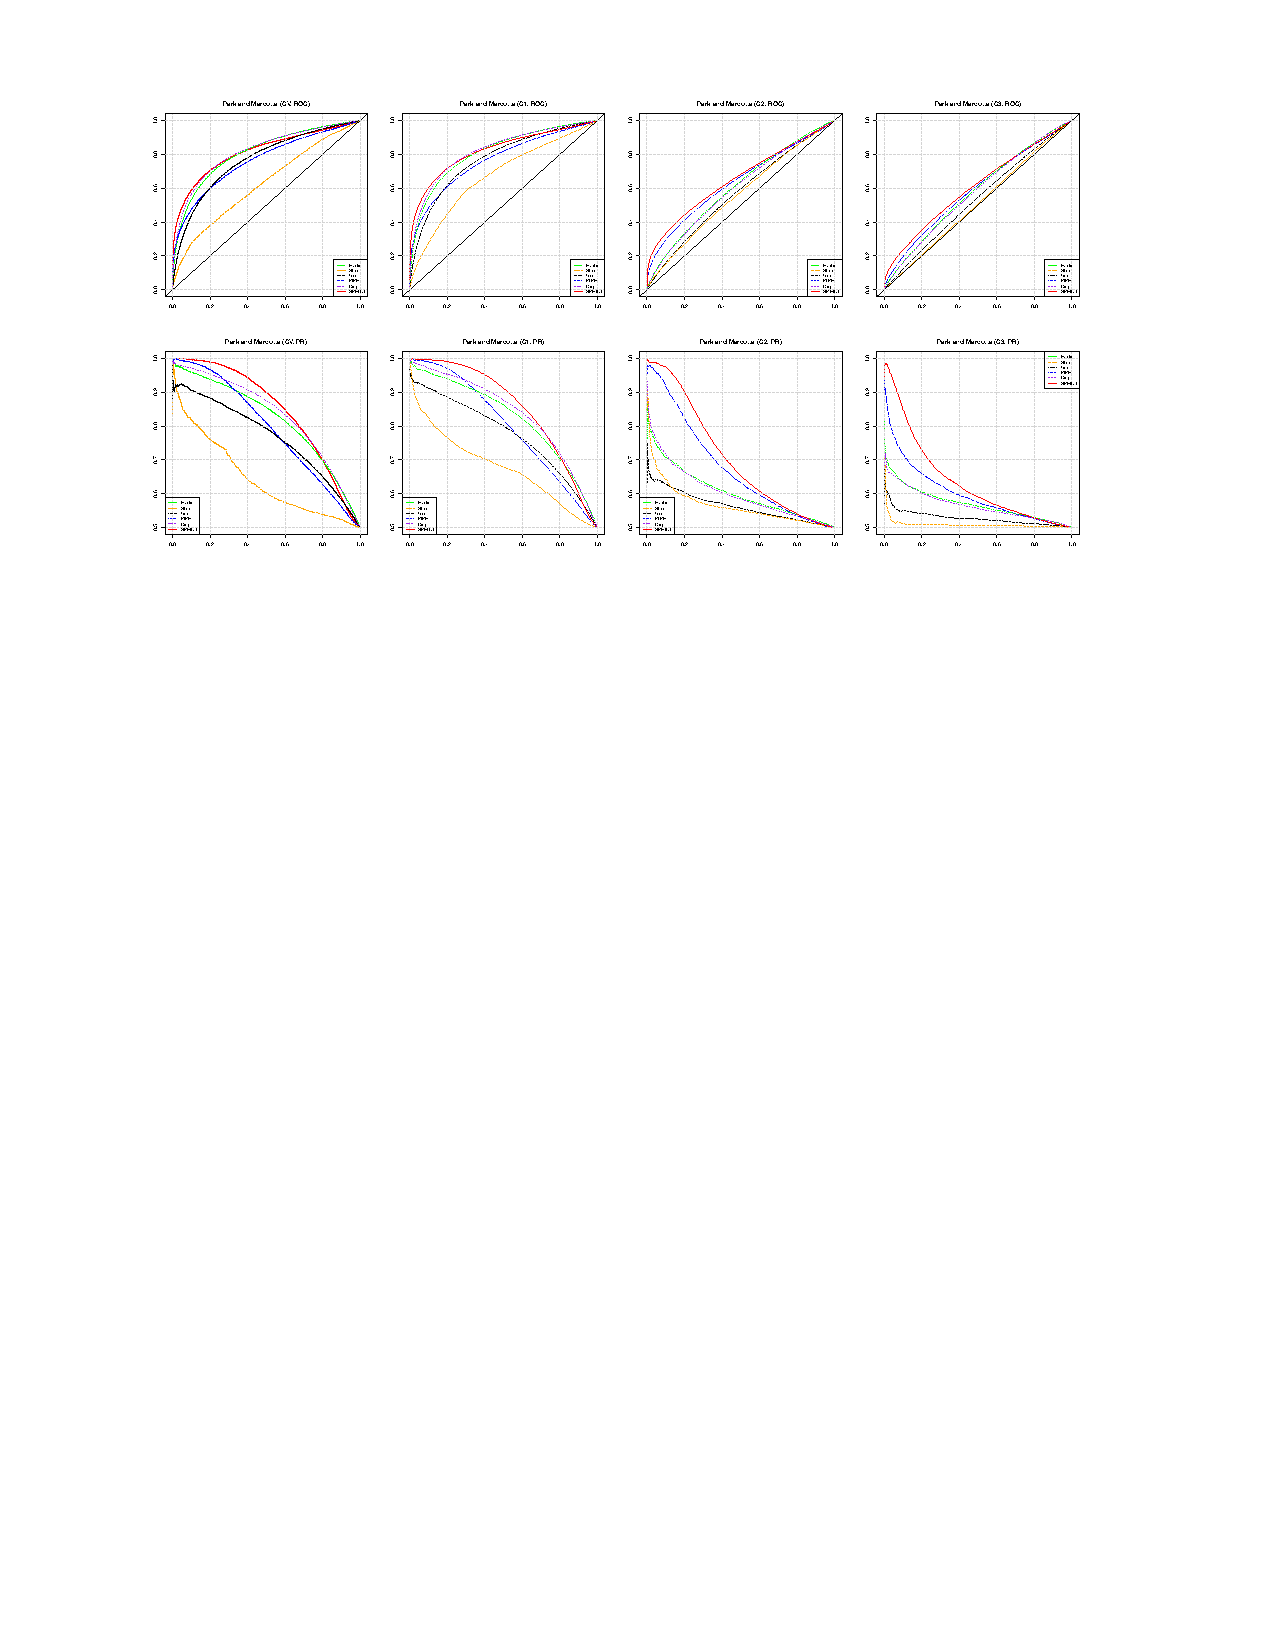
\includegraphics{img/fig_PM_plots.pdf}
  \caption[Performance comparison on Park and Marcotte datasets.]{Performance comparison on Park and Marcotte datasets. The ROC curves (top row) and PR curves (bottom row) for CV, C1, C2, and C3 datasets, from left to right. \label{fig_Park_Marcotte_curves}}
\end{figure}

The prediction performance on CV and C1 is very similar. The performance decreases from C1 to C2 and again to C3, both for ROC and PR curves. This is expected due to the way the datasets are constructed. The ROC curves do not distinguish very well between the prediction performance of the five methods. The difference is more clear in the PR curves. The SPRINT curve is almost always on top, especially at the beginning of the curve, where it matters the most for prediction. Ding's and Martin's are very close for CV and C1 datasets, followed by PIPE2. For C2 and C3 tests, the performance of Ding's and Martin's programs deteriorates and PIPE2 advances in second position.
\subsection{Comparative Analysis on Seven Human Datasets}
For a comprehensive comparison, we have compared the top four programs on six datasets, computed as mentioned above from six databases: Biogrid, HPRD Release 9, InnateDB (experimentally validated and manually curated PPIs), IntAct, and MINT. Since the prediction on the CV datasets is similar with C1, we use only C1, C2 and C3 datasets.

For the purpose of predicting new PPIs, the behaviour at high specificity is important. We therefore compare the sensitivity, precision and $F_1$-score for several high specificity values. The table with all values is given in the supplementary material. We present here in Table~\ref{table_cutoff_avg} the average values for each dataset type (C1, C2, and C3) over all datasets for each specificity value. At the bottom of the table we give also the average over all three dataset types. The performance of SPRINT with respect to all three measures, sensitivity, precision, and $F_1$-score is the highest. Only Ding comes close for C1 datasets. the overall average of SPRINT is much higher than Ding's. PIPE2 comes third and Martin last. The performance of PIPE2 decreases much less from C1 to C3 compared with Ding's. It should be noted that a weighted overall average, where the contribution of each dataset type C1,2,3 is proportional with its share of the general population, would place PIPE2 slightly ahead of Ding.

The area under the ROC and PR curves is given in Table~\ref{table_AUC} for all seven datasets, including the C1-, C2-, and C3-average, as well as the overall average across types. Ding is the winner for the C1 tests and SPRINT is the winner for the C2 and C3 tests. In the overall average, SPRINT comes on top. Martin is third and PIPE2 last.

All ROC and PR curves are included in the supplementary material.
\begin{landscape}
\begin{table} 
  \centering
  
\caption[Performance comparison at high specificity]{Performance comparison at high specificity. Sensitivity, precision, and $F_1$-score averages for seven datasets are given for each dataset type C1, C2 and C3, as well as overall averages across types. Darker colours represent better results. The best results are in bold. \label{table_cutoff_avg}} 
\fontsize{9.5}{8}\selectfont
% \begin{adjustwidth}{-2.5cm}{}
    \begin{tabular}{|@{}c@{}|@{\ }c@{\ }|cccc|cccc|cccc|}
    \toprule
    \multirow{2}[4]{*}{\textbf{Dataset}} & \multirow{2}[4]{*}{\textbf{Specificity}} & \multicolumn{4}{c|}{\textbf{Sensitivity}} & \multicolumn{4}{c|}{\textbf{Precision}} & \multicolumn{4}{c|}{\textbf{F1-score}} \\
\cmidrule{3-14}          &       & \textbf{$\!\!\!$Martin$\!\!\!$} & \textbf{$\!\!\!$PIPE2$\!\!\!$} & \textbf{$\!\!\!$Ding$\!\!\!$} & \textbf{$\!\!\!$SPRINT$\!\!\!$} & \textbf{$\!\!\!$Martin$\!\!\!$} & \textbf{$\!\!\!$PIPE2$\!\!\!$} & \textbf{$\!\!\!$Ding$\!\!\!$} & \textbf{$\!\!\!$SPRINT$\!\!\!$} & \textbf{$\!\!\!$Martin$\!\!\!$} & \textbf{$\!\!\!$PIPE2$\!\!\!$} & \textbf{$\!\!\!$Ding$\!\!\!$} & \textbf{$\!\!\!$SPRINT$\!\!\!$} \\
    \midrule
    \multirow{5}[2]{*}{\begin{tabular}{c}\textbf{C1}\\ \textbf{average}\end{tabular}} & 99.95\% & \cellcolor[rgb]{ .886,  .937,  .855} 6.07 & \cellcolor[rgb]{ .773,  .851,  .722} 7.60 & \cellcolor[rgb]{ .439,  .596,  .337} 11.93 & \cellcolor[rgb]{ .329,  .51,  .208} 13.35 & \cellcolor[rgb]{ .373,  .545,  .259} 98.52 & \cellcolor[rgb]{ .357,  .533,  .239} 98.82 & \cellcolor[rgb]{ .886,  .937,  .855} 88.05 & \cellcolor[rgb]{ .329,  .51,  .208} 99.37 & \cellcolor[rgb]{ .886,  .937,  .855} 11.06 & \cellcolor[rgb]{ .773,  .851,  .722} 13.55 & \cellcolor[rgb]{ .451,  .604,  .349} 20.39 & \cellcolor[rgb]{ .329,  .51,  .208} 22.93 \\
          & 99.90\% & \cellcolor[rgb]{ .886,  .937,  .855} 6.53 & \cellcolor[rgb]{ .729,  .82,  .675} 9.20 & \cellcolor[rgb]{ .431,  .588,  .325} 14.24 & \cellcolor[rgb]{ .329,  .51,  .208} 15.91 & \cellcolor[rgb]{ .455,  .608,  .353} 97.36 & \cellcolor[rgb]{ .376,  .545,  .263} 98.61 & \cellcolor[rgb]{ .886,  .937,  .855} 90.65 & \cellcolor[rgb]{ .329,  .51,  .208} 99.29 & \cellcolor[rgb]{ .886,  .937,  .855} 11.88 & \cellcolor[rgb]{ .722,  .812,  .663} 16.45 & \cellcolor[rgb]{ .439,  .596,  .333} 24.10 & \cellcolor[rgb]{ .329,  .51,  .208} 27.03 \\
          & 99.50\% & \cellcolor[rgb]{ .886,  .937,  .855} 17.27 & \cellcolor[rgb]{ .706,  .8,  .643} 21.41 & \cellcolor[rgb]{ .329,  .51,  .208} 29.90 & \cellcolor[rgb]{ .349,  .525,  .231} 29.50 & \cellcolor[rgb]{ .886,  .937,  .855} 96.66 & \cellcolor[rgb]{ .596,  .718,  .518} 97.52 & \cellcolor[rgb]{ .365,  .537,  .247} 98.20 & \cellcolor[rgb]{ .329,  .51,  .208} 98.30 & \cellcolor[rgb]{ .886,  .937,  .855} 28.62 & \cellcolor[rgb]{ .682,  .78,  .62} 34.73 & \cellcolor[rgb]{ .333,  .514,  .212} 45.19 & \cellcolor[rgb]{ .329,  .51,  .208} 45.22 \\
          & 99.00\% & \cellcolor[rgb]{ .886,  .937,  .855} 25.48 & \cellcolor[rgb]{ .765,  .843,  .714} 28.73 & \cellcolor[rgb]{ .384,  .553,  .271} 38.72 & \cellcolor[rgb]{ .329,  .51,  .208} 40.14 & \cellcolor[rgb]{ .886,  .937,  .855} 95.55 & \cellcolor[rgb]{ .647,  .753,  .576} 96.40 & \cellcolor[rgb]{ .396,  .561,  .286} 97.28 & \cellcolor[rgb]{ .329,  .51,  .208} 97.52 & \cellcolor[rgb]{ .886,  .937,  .855} 39.14 & \cellcolor[rgb]{ .741,  .827,  .686} 43.69 & \cellcolor[rgb]{ .392,  .557,  .278} 54.69 & \cellcolor[rgb]{ .329,  .51,  .208} 56.58 \\
          & 95.00\% & \cellcolor[rgb]{ .659,  .761,  .588} 55.35 & \cellcolor[rgb]{ .886,  .937,  .855} 48.07 & \cellcolor[rgb]{ .329,  .51,  .208} 65.68 & \cellcolor[rgb]{ .447,  .6,  .345} 62.02 & \cellcolor[rgb]{ .616,  .729,  .537} 91.44 & \cellcolor[rgb]{ .886,  .937,  .855} 90.19 & \cellcolor[rgb]{ .329,  .51,  .208} 92.72 & \cellcolor[rgb]{ .4,  .565,  .29} 92.41 & \cellcolor[rgb]{ .643,  .753,  .573} 68.37 & \cellcolor[rgb]{ .886,  .937,  .855} 62.09 & \cellcolor[rgb]{ .329,  .51,  .208} 76.41 & \cellcolor[rgb]{ .427,  .588,  .322} 73.90 \\
    \midrule
    \multirow{5}[2]{*}{\begin{tabular}{c}\textbf{C2}\\ \textbf{average}\end{tabular}} & 99.95\% & \cellcolor[rgb]{ .886,  .937,  .855} 5.55 & \cellcolor[rgb]{ .71,  .804,  .651} 10.65 & \cellcolor[rgb]{ .761,  .839,  .706} 9.22 & \cellcolor[rgb]{ .329,  .51,  .208} 21.45 & \cellcolor[rgb]{ .886,  .937,  .855} 96.33 & \cellcolor[rgb]{ .365,  .537,  .247} 99.42 & \cellcolor[rgb]{ .62,  .733,  .541} 97.92 & \cellcolor[rgb]{ .329,  .51,  .208} 99.62 & \cellcolor[rgb]{ .886,  .937,  .855} 9.78 & \cellcolor[rgb]{ .671,  .773,  .604} 18.91 & \cellcolor[rgb]{ .773,  .851,  .722} 14.69 & \cellcolor[rgb]{ .329,  .51,  .208} 33.16 \\
          & 99.90\% & \cellcolor[rgb]{ .886,  .937,  .855} 5.88 & \cellcolor[rgb]{ .718,  .808,  .659} 11.28 & \cellcolor[rgb]{ .765,  .843,  .714} 9.78 & \cellcolor[rgb]{ .329,  .51,  .208} 23.40 & \cellcolor[rgb]{ .886,  .937,  .855} 93.66 & \cellcolor[rgb]{ .369,  .541,  .251} 98.96 & \cellcolor[rgb]{ .647,  .753,  .576} 96.11 & \cellcolor[rgb]{ .329,  .51,  .208} 99.34 & \cellcolor[rgb]{ .886,  .937,  .855} 10.40 & \cellcolor[rgb]{ .682,  .78,  .616} 19.98 & \cellcolor[rgb]{ .773,  .851,  .722} 15.70 & \cellcolor[rgb]{ .329,  .51,  .208} 36.08 \\
          & 99.50\% & \cellcolor[rgb]{ .886,  .937,  .855} 11.73 & \cellcolor[rgb]{ .682,  .78,  .616} 19.52 & \cellcolor[rgb]{ .761,  .839,  .706} 16.59 & \cellcolor[rgb]{ .329,  .51,  .208} 32.73 & \cellcolor[rgb]{ .886,  .937,  .855} 93.86 & \cellcolor[rgb]{ .475,  .62,  .376} 97.11 & \cellcolor[rgb]{ .859,  .914,  .82} 94.11 & \cellcolor[rgb]{ .329,  .51,  .208} 98.22 & \cellcolor[rgb]{ .886,  .937,  .855} 20.17 & \cellcolor[rgb]{ .651,  .757,  .584} 31.86 & \cellcolor[rgb]{ .757,  .839,  .706} 26.59 & \cellcolor[rgb]{ .329,  .51,  .208} 47.77 \\
          & 99.00\% & \cellcolor[rgb]{ .886,  .937,  .855} 15.03 & \cellcolor[rgb]{ .643,  .753,  .573} 24.93 & \cellcolor[rgb]{ .702,  .796,  .643} 22.55 & \cellcolor[rgb]{ .329,  .51,  .208} 37.60 & \cellcolor[rgb]{ .886,  .937,  .855} 91.85 & \cellcolor[rgb]{ .482,  .627,  .388} 95.64 & \cellcolor[rgb]{ .71,  .804,  .651} 93.52 & \cellcolor[rgb]{ .329,  .51,  .208} 97.07 & \cellcolor[rgb]{ .886,  .937,  .855} 25.26 & \cellcolor[rgb]{ .616,  .729,  .541} 38.84 & \cellcolor[rgb]{ .694,  .788,  .631} 34.94 & \cellcolor[rgb]{ .329,  .51,  .208} 52.97 \\
          & 95.00\% & \cellcolor[rgb]{ .886,  .937,  .855} 37.41 & \cellcolor[rgb]{ .765,  .843,  .71} 40.95 & \cellcolor[rgb]{ .663,  .765,  .592} 43.83 & \cellcolor[rgb]{ .329,  .51,  .208} 53.17 & \cellcolor[rgb]{ .886,  .937,  .855} 86.45 & \cellcolor[rgb]{ .631,  .741,  .561} 88.43 & \cellcolor[rgb]{ .655,  .757,  .584} 88.27 & \cellcolor[rgb]{ .329,  .51,  .208} 90.76 & \cellcolor[rgb]{ .886,  .937,  .855} 51.17 & \cellcolor[rgb]{ .733,  .82,  .678} 55.33 & \cellcolor[rgb]{ .647,  .753,  .576} 57.69 & \cellcolor[rgb]{ .329,  .51,  .208} 66.18 \\
    \midrule
    \multirow{5}[2]{*}{\begin{tabular}{c}\textbf{C3}\\ \textbf{average}\end{tabular}} & 99.95\% & \cellcolor[rgb]{ .886,  .937,  .855} 1.04 & \cellcolor[rgb]{ .847,  .91,  .812} 1.46 & \cellcolor[rgb]{ .851,  .91,  .812} 1.44 & \cellcolor[rgb]{ .329,  .51,  .208} 6.96 & \cellcolor[rgb]{ .663,  .769,  .596} 94.80 & \cellcolor[rgb]{ .761,  .843,  .71} 93.56 & \cellcolor[rgb]{ .886,  .937,  .855} 91.97 & \cellcolor[rgb]{ .329,  .51,  .208} 99.01 & \cellcolor[rgb]{ .886,  .937,  .855} 2.05 & \cellcolor[rgb]{ .847,  .906,  .808} 2.85 & \cellcolor[rgb]{ .851,  .91,  .812} 2.78 & \cellcolor[rgb]{ .329,  .51,  .208} 12.85 \\
          & 99.90\% & \cellcolor[rgb]{ .886,  .937,  .855} 1.20 & \cellcolor[rgb]{ .843,  .902,  .804} 1.78 & \cellcolor[rgb]{ .851,  .91,  .816} 1.65 & \cellcolor[rgb]{ .329,  .51,  .208} 8.04 & \cellcolor[rgb]{ .635,  .745,  .565} 91.31 & \cellcolor[rgb]{ .706,  .8,  .643} 89.73 & \cellcolor[rgb]{ .886,  .937,  .855} 85.41 & \cellcolor[rgb]{ .329,  .51,  .208} 98.50 & \cellcolor[rgb]{ .886,  .937,  .855} 2.37 & \cellcolor[rgb]{ .839,  .902,  .8} 3.46 & \cellcolor[rgb]{ .851,  .91,  .816} 3.18 & \cellcolor[rgb]{ .329,  .51,  .208} 14.76 \\
          & 99.50\% & \cellcolor[rgb]{ .886,  .937,  .855} 4.12 & \cellcolor[rgb]{ .867,  .922,  .831} 4.74 & \cellcolor[rgb]{ .859,  .918,  .824} 4.92 & \cellcolor[rgb]{ .329,  .51,  .208} 19.50 & \cellcolor[rgb]{ .859,  .918,  .824} 85.62 & \cellcolor[rgb]{ .694,  .792,  .631} 89.05 & \cellcolor[rgb]{ .886,  .937,  .855} 85.01 & \cellcolor[rgb]{ .329,  .51,  .208} 96.63 & \cellcolor[rgb]{ .886,  .937,  .855} 7.83 & \cellcolor[rgb]{ .863,  .918,  .827} 8.96 & \cellcolor[rgb]{ .859,  .918,  .824} 9.03 & \cellcolor[rgb]{ .329,  .51,  .208} 31.65 \\
          & 99.00\% & \cellcolor[rgb]{ .875,  .929,  .839} 7.40 & \cellcolor[rgb]{ .796,  .867,  .749} 9.89 & \cellcolor[rgb]{ .886,  .937,  .855} 6.92 & \cellcolor[rgb]{ .329,  .51,  .208} 24.81 & \cellcolor[rgb]{ .851,  .91,  .812} 83.64 & \cellcolor[rgb]{ .678,  .776,  .612} 87.41 & \cellcolor[rgb]{ .886,  .937,  .855} 82.80 & \cellcolor[rgb]{ .329,  .51,  .208} 94.99 & \cellcolor[rgb]{ .867,  .922,  .831} 13.51 & \cellcolor[rgb]{ .784,  .859,  .737} 17.32 & \cellcolor[rgb]{ .886,  .937,  .855} 12.48 & \cellcolor[rgb]{ .329,  .51,  .208} 38.32 \\
          & 95.00\% & \cellcolor[rgb]{ .867,  .922,  .831} 24.82 & \cellcolor[rgb]{ .776,  .851,  .725} 27.35 & \cellcolor[rgb]{ .886,  .937,  .855} 24.18 & \cellcolor[rgb]{ .329,  .51,  .208} 39.79 & \cellcolor[rgb]{ .886,  .937,  .855} 80.99 & \cellcolor[rgb]{ .769,  .847,  .718} 82.36 & \cellcolor[rgb]{ .878,  .929,  .843} 81.13 & \cellcolor[rgb]{ .329,  .51,  .208} 87.38 & \cellcolor[rgb]{ .859,  .918,  .824} 37.59 & \cellcolor[rgb]{ .773,  .851,  .722} 40.28 & \cellcolor[rgb]{ .886,  .937,  .855} 36.73 & \cellcolor[rgb]{ .329,  .51,  .208} 53.82 \\
    \midrule
    \multirow{5}[2]{*}{\begin{tabular}{c}\textbf{Overall}\\ \textbf{AVERAGE}\end{tabular}} & 99.95\% & \cellcolor[rgb]{ .886,  .937,  .855} 4.22 & \cellcolor[rgb]{ .753,  .835,  .702} 6.57 & \cellcolor[rgb]{ .698,  .792,  .635} 7.53 & \cellcolor[rgb]{ .329,  .51,  .208} 13.92 & \cellcolor[rgb]{ .565,  .69,  .478} 96.55 & \cellcolor[rgb]{ .502,  .643,  .408} 97.27 & \cellcolor[rgb]{ .886,  .937,  .855} 92.65 & \cellcolor[rgb]{ .329,  .51,  .208} 99.33 & \cellcolor[rgb]{ .886,  .937,  .855} 7.63 & \cellcolor[rgb]{ .737,  .824,  .682} 11.77 & \cellcolor[rgb]{ .706,  .8,  .647} 12.62 & \cellcolor[rgb]{ .329,  .51,  .208} 22.98 \\
          & 99.90\% & \cellcolor[rgb]{ .886,  .937,  .855} 4.54 & \cellcolor[rgb]{ .745,  .831,  .69} 7.42 & \cellcolor[rgb]{ .69,  .788,  .627} 8.56 & \cellcolor[rgb]{ .329,  .51,  .208} 15.79 & \cellcolor[rgb]{ .663,  .765,  .592} 94.11 & \cellcolor[rgb]{ .549,  .678,  .463} 95.77 & \cellcolor[rgb]{ .886,  .937,  .855} 90.73 & \cellcolor[rgb]{ .329,  .51,  .208} 99.04 & \cellcolor[rgb]{ .886,  .937,  .855} 8.22 & \cellcolor[rgb]{ .729,  .816,  .671} 13.30 & \cellcolor[rgb]{ .698,  .792,  .635} 14.33 & \cellcolor[rgb]{ .329,  .51,  .208} 25.96 \\
          & 99.50\% & \cellcolor[rgb]{ .886,  .937,  .855} 11.04 & \cellcolor[rgb]{ .745,  .827,  .69} 15.23 & \cellcolor[rgb]{ .678,  .776,  .612} 17.14 & \cellcolor[rgb]{ .329,  .51,  .208} 27.24 & \cellcolor[rgb]{ .886,  .937,  .855} 92.05 & \cellcolor[rgb]{ .643,  .749,  .569} 94.56 & \cellcolor[rgb]{ .851,  .91,  .812} 92.44 & \cellcolor[rgb]{ .329,  .51,  .208} 97.71 & \cellcolor[rgb]{ .886,  .937,  .855} 18.87 & \cellcolor[rgb]{ .733,  .82,  .678} 25.18 & \cellcolor[rgb]{ .69,  .788,  .627} 26.94 & \cellcolor[rgb]{ .329,  .51,  .208} 41.54 \\
          & 99.00\% & \cellcolor[rgb]{ .886,  .937,  .855} 15.97 & \cellcolor[rgb]{ .729,  .816,  .671} 21.19 & \cellcolor[rgb]{ .682,  .78,  .616} 22.73 & \cellcolor[rgb]{ .329,  .51,  .208} 34.18 & \cellcolor[rgb]{ .886,  .937,  .855} 90.35 & \cellcolor[rgb]{ .635,  .745,  .565} 93.15 & \cellcolor[rgb]{ .812,  .878,  .769} 91.20 & \cellcolor[rgb]{ .329,  .51,  .208} 96.52 & \cellcolor[rgb]{ .886,  .937,  .855} 25.97 & \cellcolor[rgb]{ .714,  .804,  .655} 33.28 & \cellcolor[rgb]{ .694,  .792,  .631} 34.04 & \cellcolor[rgb]{ .329,  .51,  .208} 49.29 \\
          & 95.00\% & \cellcolor[rgb]{ .871,  .925,  .835} 39.19 & \cellcolor[rgb]{ .886,  .937,  .855} 38.79 & \cellcolor[rgb]{ .639,  .749,  .565} 44.56 & \cellcolor[rgb]{ .329,  .51,  .208} 51.66 & \cellcolor[rgb]{ .886,  .937,  .855} 86.30 & \cellcolor[rgb]{ .788,  .863,  .741} 86.99 & \cellcolor[rgb]{ .733,  .82,  .678} 87.37 & \cellcolor[rgb]{ .329,  .51,  .208} 90.18 & \cellcolor[rgb]{ .886,  .937,  .855} 52.38 & \cellcolor[rgb]{ .878,  .933,  .847} 52.57 & \cellcolor[rgb]{ .682,  .78,  .616} 56.94 & \cellcolor[rgb]{ .329,  .51,  .208} 64.63 \\
    \bottomrule
    \end{tabular}%
    % \end{adjustwidth}
\end{table}%
\end{landscape}


\begin{table}[] 
%   \centering
\caption[Area under curves]{Area under curves. AUROC and AUPR curves are given for seven datasets and three types, C1, C2, C3, for each, as well as averages for each type and overall average across types. Darker colours represent better results. The best results are in bold. \label{table_AUC}} 
    \begin{tabular}{|c|cccc|cccc|}
    \toprule
    \multirow{3}[6]{*}{\textbf{Dataset}} & \multicolumn{4}{c|}{\textbf{AUROC}} & \multicolumn{4}{c|}{\textbf{AUPR}} \\
\cmidrule{2-9}          & \textbf{$\!\!\!$Martin$\!\!\!$} & \textbf{$\!\!\!$PIPE2$\!\!\!$} & \textbf{$\!\!\!$Ding$\!\!\!$} & \textbf{$\!\!\!$SPRINT$\!\!\!$} & \textbf{$\!\!\!$Martin$\!\!\!$} & \textbf{$\!\!\!$PIPE2$\!\!\!$} & \textbf{$\!\!\!$Ding$\!\!\!$} & \textbf{$\!\!\!$SPRINT$\!\!\!$} \\
\cmidrule{2-9}          & \multicolumn{8}{c|}{\textbf{C1}} \\
    \midrule
    \textbf{Biogrid} & \cellcolor[rgb]{ .549,  .678,  .463} 87.54 & \cellcolor[rgb]{ .886,  .937,  .855} 79.01 & \cellcolor[rgb]{ .329,  .51,  .208} 93.06 & \cellcolor[rgb]{ .529,  .663,  .439} 88.11 & \cellcolor[rgb]{ .592,  .714,  .514} 87.20 & \cellcolor[rgb]{ .886,  .937,  .855} 80.52 & \cellcolor[rgb]{ .329,  .51,  .208} 93.08 & \cellcolor[rgb]{ .502,  .643,  .408} 89.24 \\
    \textbf{HPRD} & \cellcolor[rgb]{ .51,  .651,  .42} 86.83 & \cellcolor[rgb]{ .886,  .937,  .855} 81.53 & \cellcolor[rgb]{ .329,  .51,  .208} 89.34 & \cellcolor[rgb]{ .514,  .655,  .424} 86.76 & \cellcolor[rgb]{ .639,  .749,  .569} 86.93 & \cellcolor[rgb]{ .886,  .937,  .855} 84.31 & \cellcolor[rgb]{ .329,  .51,  .208} 90.20 & \cellcolor[rgb]{ .416,  .576,  .306} 89.32 \\
    \textbf{Innate\_Exp} & \cellcolor[rgb]{ .537,  .671,  .451} 90.18 & \cellcolor[rgb]{ .886,  .937,  .855} 83.98 & \cellcolor[rgb]{ .329,  .51,  .208} 93.83 & \cellcolor[rgb]{ .471,  .62,  .373} 91.34 & \cellcolor[rgb]{ .576,  .702,  .494} 90.31 & \cellcolor[rgb]{ .886,  .937,  .855} 85.48 & \cellcolor[rgb]{ .329,  .51,  .208} 94.14 & \cellcolor[rgb]{ .455,  .604,  .353} 92.25 \\
    \textbf{Innate\_Man} & \cellcolor[rgb]{ .424,  .584,  .318} 94.11 & \cellcolor[rgb]{ .886,  .937,  .855} 90.26 & \cellcolor[rgb]{ .329,  .51,  .208} 94.89 & \cellcolor[rgb]{ .549,  .678,  .463} 93.09 & \cellcolor[rgb]{ .459,  .608,  .357} 94.93 & \cellcolor[rgb]{ .886,  .937,  .855} 92.22 & \cellcolor[rgb]{ .329,  .51,  .208} 95.73 & \cellcolor[rgb]{ .486,  .631,  .392} 94.75 \\
    \textbf{IntAct} & \cellcolor[rgb]{ .533,  .667,  .443} 88.02 & \cellcolor[rgb]{ .886,  .937,  .855} 80.72 & \cellcolor[rgb]{ .329,  .51,  .208} 92.18 & \cellcolor[rgb]{ .502,  .643,  .408} 88.69 & \cellcolor[rgb]{ .584,  .706,  .502} 87.51 & \cellcolor[rgb]{ .886,  .937,  .855} 81.68 & \cellcolor[rgb]{ .329,  .51,  .208} 92.31 & \cellcolor[rgb]{ .467,  .616,  .369} 89.71 \\
    \textbf{MINT} & \cellcolor[rgb]{ .478,  .624,  .38} 90.86 & \cellcolor[rgb]{ .886,  .937,  .855} 83.41 & \cellcolor[rgb]{ .329,  .51,  .208} 93.54 & \cellcolor[rgb]{ .58,  .702,  .498} 89.03 & \cellcolor[rgb]{ .537,  .671,  .451} 91.08 & \cellcolor[rgb]{ .886,  .937,  .855} 85.93 & \cellcolor[rgb]{ .329,  .51,  .208} 94.11 & \cellcolor[rgb]{ .533,  .667,  .447} 91.13 \\
    \textbf{Park \& Marcotte} & \cellcolor[rgb]{ .416,  .576,  .31} 81.49 & \cellcolor[rgb]{ .886,  .937,  .855} 76.74 & \cellcolor[rgb]{ .365,  .537,  .251} 82.00 & \cellcolor[rgb]{ .329,  .51,  .208} 82.35 & \cellcolor[rgb]{ .643,  .749,  .573} 82.32 & \cellcolor[rgb]{ .886,  .937,  .855} 79.90 & \cellcolor[rgb]{ .573,  .698,  .49} 83.00 & \cellcolor[rgb]{ .329,  .51,  .208} 85.39 \\
    \midrule
          & \multicolumn{8}{c|}{\textbf{C2}} \\
    \midrule
    \textbf{Biogrid} & \cellcolor[rgb]{ .627,  .737,  .553} 81.33 & \cellcolor[rgb]{ .886,  .937,  .855} 76.66 & \cellcolor[rgb]{ .329,  .51,  .208} 86.57 & \cellcolor[rgb]{ .439,  .592,  .333} 84.67 & \cellcolor[rgb]{ .714,  .808,  .655} 80.76 & \cellcolor[rgb]{ .886,  .937,  .855} 78.25 & \cellcolor[rgb]{ .345,  .522,  .224} 86.12 & \cellcolor[rgb]{ .329,  .51,  .208} 86.30 \\
    \textbf{HPRD} & \cellcolor[rgb]{ .675,  .776,  .608} 83.30 & \cellcolor[rgb]{ .886,  .937,  .855} 81.55 & \cellcolor[rgb]{ .49,  .635,  .396} 84.78 & \cellcolor[rgb]{ .329,  .51,  .208} 86.09 & \cellcolor[rgb]{ .886,  .937,  .855} 82.85 & \cellcolor[rgb]{ .773,  .851,  .725} 83.98 & \cellcolor[rgb]{ .686,  .784,  .624} 84.85 & \cellcolor[rgb]{ .329,  .51,  .208} 88.37 \\
    \textbf{Innate\_Exp} & \cellcolor[rgb]{ .71,  .804,  .651} 83.96 & \cellcolor[rgb]{ .886,  .937,  .855} 81.46 & \cellcolor[rgb]{ .424,  .584,  .318} 87.98 & \cellcolor[rgb]{ .329,  .51,  .208} 89.31 & \cellcolor[rgb]{ .804,  .875,  .761} 83.74 & \cellcolor[rgb]{ .886,  .937,  .855} 82.57 & \cellcolor[rgb]{ .506,  .647,  .416} 87.91 & \cellcolor[rgb]{ .329,  .51,  .208} 90.37 \\
    \textbf{Innate\_Man} & \cellcolor[rgb]{ .639,  .749,  .565} 85.87 & \cellcolor[rgb]{ .886,  .937,  .855} 84.43 & \cellcolor[rgb]{ .835,  .898,  .796} 84.74 & \cellcolor[rgb]{ .329,  .51,  .208} 87.64 & \cellcolor[rgb]{ .784,  .859,  .733} 87.71 & \cellcolor[rgb]{ .867,  .922,  .831} 87.22 & \cellcolor[rgb]{ .886,  .937,  .855} 87.10 & \cellcolor[rgb]{ .329,  .51,  .208} 90.33 \\
    \textbf{IntAct} & \cellcolor[rgb]{ .608,  .722,  .529} 81.68 & \cellcolor[rgb]{ .886,  .937,  .855} 77.64 & \cellcolor[rgb]{ .329,  .51,  .208} 85.63 & \cellcolor[rgb]{ .506,  .643,  .412} 83.14 & \cellcolor[rgb]{ .725,  .816,  .671} 80.68 & \cellcolor[rgb]{ .886,  .937,  .855} 78.69 & \cellcolor[rgb]{ .361,  .533,  .243} 85.20 & \cellcolor[rgb]{ .329,  .51,  .208} 85.58 \\
    \textbf{MINT} & \cellcolor[rgb]{ .384,  .553,  .271} 86.66 & \cellcolor[rgb]{ .886,  .937,  .855} 81.76 & \cellcolor[rgb]{ .329,  .51,  .208} 87.17 & \cellcolor[rgb]{ .431,  .588,  .325} 86.20 & \cellcolor[rgb]{ .6,  .718,  .522} 86.37 & \cellcolor[rgb]{ .886,  .937,  .855} 84.08 & \cellcolor[rgb]{ .459,  .608,  .357} 87.47 & \cellcolor[rgb]{ .329,  .51,  .208} 88.47 \\
    \textbf{Park \& Marcotte} & \cellcolor[rgb]{ .82,  .886,  .776} 60.67 & \cellcolor[rgb]{ .51,  .647,  .416} 63.76 & \cellcolor[rgb]{ .886,  .937,  .855} 60.00 & \cellcolor[rgb]{ .329,  .51,  .208} 65.52 & \cellcolor[rgb]{ .867,  .922,  .831} 60.43 & \cellcolor[rgb]{ .486,  .631,  .388} 67.41 & \cellcolor[rgb]{ .886,  .937,  .855} 60.00 & \cellcolor[rgb]{ .329,  .51,  .208} 70.25 \\
    \midrule
          & \multicolumn{8}{c|}{\textbf{C3}} \\
    \midrule
    \textbf{Biogrid} & \cellcolor[rgb]{ .565,  .69,  .482} 76.20 & \cellcolor[rgb]{ .886,  .937,  .855} 71.38 & \cellcolor[rgb]{ .365,  .537,  .251} 79.16 & \cellcolor[rgb]{ .329,  .51,  .208} 79.67 & \cellcolor[rgb]{ .639,  .749,  .565} 74.89 & \cellcolor[rgb]{ .886,  .937,  .855} 70.25 & \cellcolor[rgb]{ .51,  .651,  .42} 77.24 & \cellcolor[rgb]{ .329,  .51,  .208} 80.59 \\
    \textbf{HPRD} & \cellcolor[rgb]{ .678,  .776,  .612} 79.46 & \cellcolor[rgb]{ .886,  .937,  .855} 77.14 & \cellcolor[rgb]{ .855,  .914,  .816} 77.51 & \cellcolor[rgb]{ .329,  .51,  .208} 83.27 & \cellcolor[rgb]{ .706,  .8,  .647} 78.51 & \cellcolor[rgb]{ .718,  .808,  .659} 78.28 & \cellcolor[rgb]{ .886,  .937,  .855} 75.32 & \cellcolor[rgb]{ .329,  .51,  .208} 85.08 \\
    \textbf{Innate\_Exp} & \cellcolor[rgb]{ .765,  .843,  .71} 78.10 & \cellcolor[rgb]{ .886,  .937,  .855} 75.89 & \cellcolor[rgb]{ .616,  .729,  .541} 80.69 & \cellcolor[rgb]{ .329,  .51,  .208} 85.70 & \cellcolor[rgb]{ .784,  .859,  .733} 76.65 & \cellcolor[rgb]{ .886,  .937,  .855} 74.42 & \cellcolor[rgb]{ .694,  .788,  .631} 78.55 & \cellcolor[rgb]{ .329,  .51,  .208} 86.23 \\
    \textbf{Innate\_Man} & \cellcolor[rgb]{ .584,  .706,  .502} 71.75 & \cellcolor[rgb]{ .506,  .647,  .412} 73.25 & \cellcolor[rgb]{ .886,  .937,  .855} 65.96 & \cellcolor[rgb]{ .329,  .51,  .208} 76.57 & \cellcolor[rgb]{ .612,  .725,  .533} 73.49 & \cellcolor[rgb]{ .549,  .678,  .463} 74.95 & \cellcolor[rgb]{ .886,  .937,  .855} 66.81 & \cellcolor[rgb]{ .329,  .51,  .208} 80.17 \\
    \textbf{IntAct} & \cellcolor[rgb]{ .533,  .667,  .443} 76.94 & \cellcolor[rgb]{ .886,  .937,  .855} 73.61 & \cellcolor[rgb]{ .329,  .51,  .208} 78.81 & \cellcolor[rgb]{ .8,  .871,  .753} 74.44 & \cellcolor[rgb]{ .69,  .788,  .627} 74.88 & \cellcolor[rgb]{ .886,  .937,  .855} 73.11 & \cellcolor[rgb]{ .561,  .686,  .475} 76.03 & \cellcolor[rgb]{ .329,  .51,  .208} 78.08 \\
    \textbf{MINT} & \cellcolor[rgb]{ .49,  .635,  .396} 81.25 & \cellcolor[rgb]{ .886,  .937,  .855} 78.06 & \cellcolor[rgb]{ .78,  .855,  .729} 78.94 & \cellcolor[rgb]{ .329,  .51,  .208} 82.54 & \cellcolor[rgb]{ .667,  .769,  .6} 80.07 & \cellcolor[rgb]{ .729,  .816,  .671} 79.28 & \cellcolor[rgb]{ .886,  .937,  .855} 77.14 & \cellcolor[rgb]{ .329,  .51,  .208} 84.55 \\
    \textbf{Park \& Marcotte} & \cellcolor[rgb]{ .757,  .835,  .702} 57.86 & \cellcolor[rgb]{ .596,  .714,  .514} 58.90 & \cellcolor[rgb]{ .886,  .937,  .855} 57.00 & \cellcolor[rgb]{ .329,  .51,  .208} 60.60 & \cellcolor[rgb]{ .808,  .878,  .765} 57.07 & \cellcolor[rgb]{ .604,  .722,  .525} 59.84 & \cellcolor[rgb]{ .886,  .937,  .855} 56.00 & \cellcolor[rgb]{ .329,  .51,  .208} 63.49 \\
    \midrule
          & \multicolumn{8}{c|}{\textbf{AVERAGES}} \\
    \midrule
    \textbf{C1 average} & \cellcolor[rgb]{ .506,  .647,  .412} 88.43 & \cellcolor[rgb]{ .886,  .937,  .855} 82.24 & \cellcolor[rgb]{ .329,  .51,  .208} 91.26 & \cellcolor[rgb]{ .502,  .643,  .408} 88.48 & \cellcolor[rgb]{ .569,  .694,  .486} 88.61 & \cellcolor[rgb]{ .886,  .937,  .855} 84.29 & \cellcolor[rgb]{ .329,  .51,  .208} 91.80 & \cellcolor[rgb]{ .447,  .6,  .341} 90.26 \\
\cmidrule{1-1}    \textbf{C2 average} & \cellcolor[rgb]{ .631,  .741,  .561} 80.50 & \cellcolor[rgb]{ .886,  .937,  .855} 78.18 & \cellcolor[rgb]{ .42,  .58,  .314} 82.41 & \cellcolor[rgb]{ .329,  .51,  .208} 83.23 & \cellcolor[rgb]{ .882,  .937,  .851} 80.36 & \cellcolor[rgb]{ .886,  .937,  .855} 80.32 & \cellcolor[rgb]{ .643,  .753,  .573} 82.67 & \cellcolor[rgb]{ .329,  .51,  .208} 85.67 \\
\cmidrule{1-1}    \textbf{C3 average} & \cellcolor[rgb]{ .675,  .773,  .608} 74.51 & \cellcolor[rgb]{ .886,  .937,  .855} 72.60 & \cellcolor[rgb]{ .729,  .816,  .671} 74.01 & \cellcolor[rgb]{ .329,  .51,  .208} 77.54 & \cellcolor[rgb]{ .796,  .867,  .749} 73.65 & \cellcolor[rgb]{ .855,  .914,  .82} 72.88 & \cellcolor[rgb]{ .886,  .937,  .855} 72.44 & \cellcolor[rgb]{ .329,  .51,  .208} 79.74 \\
    \midrule
    \textbf{Overall AVERAGE} & \cellcolor[rgb]{ .529,  .667,  .443} 81.15 & \cellcolor[rgb]{ .886,  .937,  .855} 77.67 & \cellcolor[rgb]{ .384,  .553,  .271} 82.56 & \cellcolor[rgb]{ .329,  .51,  .208} 83.08 & \cellcolor[rgb]{ .729,  .82,  .675} 80.87 & \cellcolor[rgb]{ .886,  .937,  .855} 79.16 & \cellcolor[rgb]{ .6,  .718,  .522} 82.30 & \cellcolor[rgb]{ .329,  .51,  .208} 85.22 \\
    \bottomrule
    \end{tabular}%
\end{table}%
\subsection{Comparative Analysis on Human Interactome Prediction}
The goal of all PPI prediction methods is to predict new interactions from existing reliable ones. That means, in practice we input all known interactions -- the entire interactome of an organism -- and predict new ones. Of the newly predicted interactions, only those that are the most likely to be true interactions are kept. 

For predicting the entire interactome, we need to predict the probability of interaction between any two proteins. Recall that for $P$ proteins, that means we need to consider $(1+P)\times P\div2$ protein pairs. For our 20,160 proteins, that is about 203 million potential interactions. %; 203,222,880
For example, predicting one pair per second results in over six years of computation time. 

We have tested the four programs, Martin's, PIPE2, Ding's, and SPRINT, on the entire human interactome, considering as given PPIs each of the six datasets in Table~\ref{table_datasets}. The tests were performed on a DELL PowerEdge R620 computer with 12 cores Intel Xeon at 2.0 GHz and 256 GB of RAM, running Linux Red Hat, CentOS 6.3. 

The time and memory values are shown in Table~\ref{table_interactome_time} for all three stages: preprocessing, training, and predicting. For each dataset, training is performed on all PPIs in that dataset and then predictions are made for all 203 million protein pairs. 

Note that PIPE2 and SPRINT do not require any training. Also, preprocessing is performed only once for all protein sequences. As long as no protein sequences are added, no preprocessing needs to be done. For SPRINT, we provide all necessary similarities for all reviewed human proteins in UniProt. If new protein sequences are added, the program has an option (``\texttt{-add}'') that is able to compute only the new similarities, which is very fast.

Therefore, the comparison is between predicting time of PIPE2 and SPRINT and training plus predicting time of Martin and Ding. PIPE2 and Martin are very slow and the predicting times are estimated by running the programs for 100 hours and then estimating according to the number of protein pairs left to process. Both take too long to be used on the entire human interactome.

Ding's program is faster than the other two but uses a large amount of memory. It ran out of 256GB of memory when training on the two largest datasets: Biogrid and InnateDB experimentally validated. It seems able to train on the IntAct dataset but it could not finish training in 14 days, which is the longest we can run a job on our system.

SPRINT is approximately five orders of magnitude faster than PIPE2 and Martin. It is over two orders of magnitude faster than Ding but this is based on the small datasets. The results on IntAct seem to indicate that the difference increases for large datasets. 

Another interesting property of SPRINT is that it appears to scale sublinearly with the size of the datasets, that is, the larger the datasets, the faster it runs (per PPI). This means SPRINT will continue to be fast as the datasets will grow, which it is to be expected.

It should be noted that SPRINT runs in parallel whereas the other are serial. Martin's and PIPE2 are much slower, so parallelizing the prediction would not make any difference. Ding's program on the other hand uses a considerable amout of time for training, which cannot be easily parallelized. The very large difference in speed is due to the fact that while Martin, PIPE2, and Ding consider one protein pair at the time, out of the 203 million, SPRINT simply computes all 203 million scores at the same time; see the Methods section for details.

In terms of memory, SPRINT requires a very modest amount of memory to predict. We successfully ran SPRINT on all entire human interactome tests in serial mode on an older MacBook (1.4GHz processor, 4 GB RAM); the running time was between 35 minutes for Innate manually curated to 11 hours for Biogriod. 

The comparison is more visually clear in Figure~\ref{fig_time_memory} where the time (in hours) and memory are plotted together for the four programs compared and those datasets for which we have either a value or at least an estimate. Note the logarithmic scale for time. The point with the highest memory for Ding's program (for the IntAct dataset) has time value fourteen days, which is the only lower bound we have. The real time may be  much larger. 


\begin{figure}[h!]
\centering
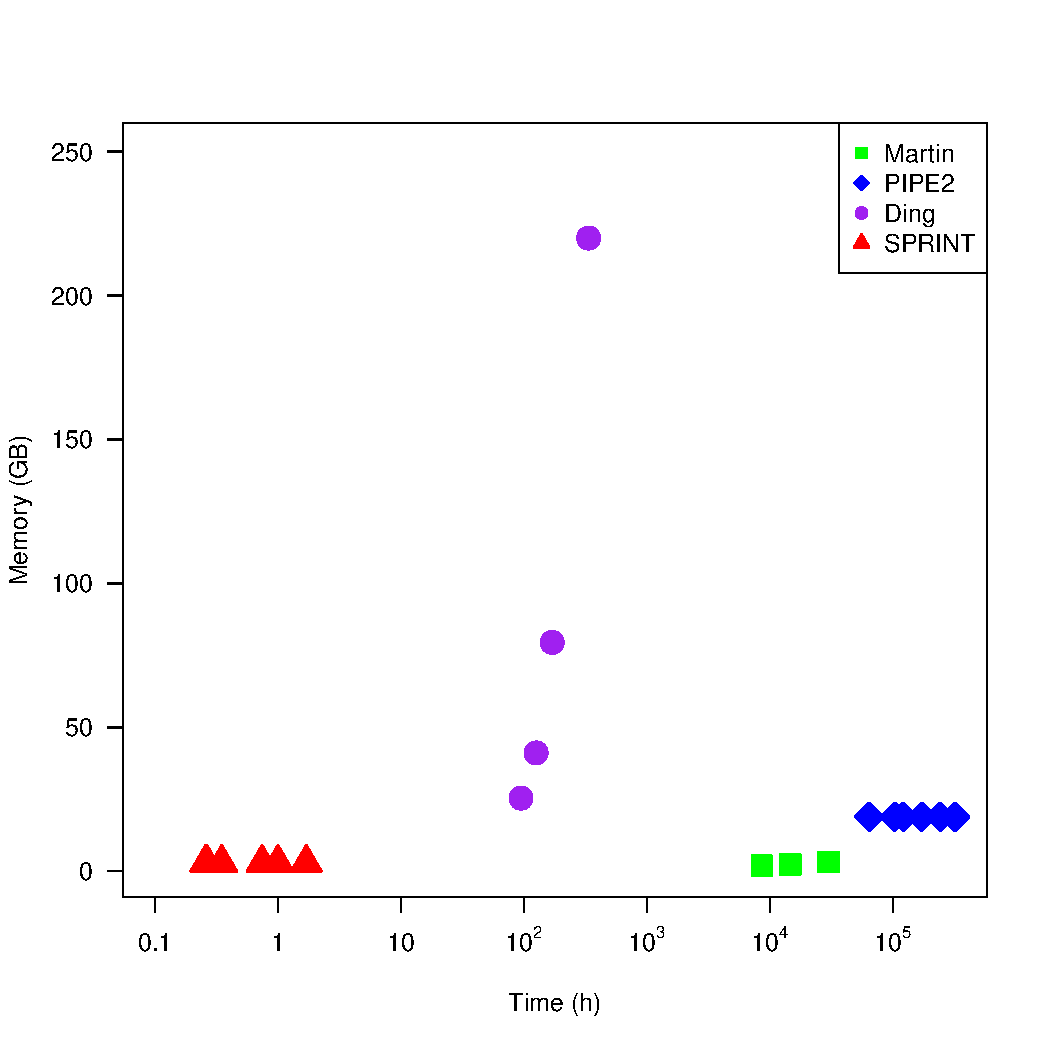
\includegraphics[width=8.5cm]{img/fig_time_memory.pdf}
\caption{Time and memory comparison for predicting the entire human interactome. \label{fig_time_memory}}
\end{figure}

\begin{table}[!h!] 
\centering
\caption[Human interactome comparison]{Human interactome comparison: running time and peak memory. The predicting time for Martin's and PIPE2 was estimated by running it for 100 hours and then estimating the total time according to the number of pairs left to predict. Note that PIPE2 and SPRINT do not require training as they are not using machine learning. For the entries marked with a dash, the program ran out of (256 GB) memory or ran for more than 14 days. Times marked with a dagger${}^\dag$ are estimated.\label{table_interactome_time}}
\begin{tabular}{@{}llrrrrrr@{}} \toprule
Dataset & Program & \multicolumn{3}{c}{Time (s)} &  \multicolumn{3}{|c}{Memory (GB)}   \\ \cmidrule{3-5} \cmidrule{6-8}
 &	& Preprocess & Train & Predict &  Preprocess & Train & Predict \\ \midrule
Biogrid & %%%%%%%%%%%%%%%%%%%%%%%%
	Martin & 32,400 & $>$ 1,209,600  & {\scriptsize  -- } & 2.5 & 6.1 & {\scriptsize  -- } \\ 
&	PIPE2 & 312,120 & {\scriptsize N$\!$/$\!$A} & ${}^\dag$1,150,675,200 & 2.1 & {\scriptsize N$\!$/$\!$A} & 18.9\\ 
&	Ding	   & 37,708 & {\scriptsize  -- } & {\scriptsize  -- }  & 3.3 &  $>$ 256 & {\scriptsize  -- }\\
&	SPRINT & 105,480 & {\scriptsize N$\!$/$\!$A} & 6,120 & 11.2 & {\scriptsize N$\!$/$\!$A} & 3.0 \\ \midrule
HPRD  & %%%%%%%%%%%%%%%%%%%%%%%% 
	Martin & 32,400 & 584,640 & ${}^\dag$107,222,400  & 2.5 & 3.2 & 1.5 \\ 
Release 9 &	PIPE2 & 312,120 & {\scriptsize N$\!$/$\!$A} & ${}^\dag$435,628,800 &  2.1 & {\scriptsize N$\!$/$\!$A} & 18.9 \\ 
&	Ding	   & 37,708 & 236,551 & 374,360 & 3.3 & 79.5 & 79.5\\
&	SPRINT & 105,480 & {\scriptsize N$\!$/$\!$A} & 1,257 & 11.2 & {\scriptsize N$\!$/$\!$A} & 3.0 \\ \midrule
Innate   & %%%%%%%%%%%%%%%%%%%%%%%%
	Martin & 32,400 & $>$ 1,209,600 & {\scriptsize  -- }  & 2.5 & 5.7 & {\scriptsize  -- } \\ 
experim. &	PIPE2 & 312,120 & {\scriptsize N$\!$/$\!$A} & ${}^\dag$872,294,400 &  2.1 &  {\scriptsize N$\!$/$\!$A} & 18.9 \\ 
validated &	Ding	   & 37,708 & {\scriptsize  -- } & {\scriptsize  -- }  & 3.3 &  $>$ 256 & {\scriptsize  -- } \\
&	SPRINT & 105,480 & {\scriptsize N$\!$/$\!$A} & 3,600 & 11.2 & {\scriptsize N$\!$/$\!$A} & 3.0  \\ \midrule
Innate  &  %%%%%%%%%%%%%%%%%%%%%%%%
	Martin & 32,400 & 26,280 & ${}^\dag$30,888,000 & 2.5 & 1.9 & 1.5 \\ 
manually &	PIPE2 & 312,120 & {\scriptsize N$\!$/$\!$A} & ${}^\dag$230,342,400  &  2.1 &  {\scriptsize N$\!$/$\!$A} & 18.9 \\ 
curated &	Ding	   & 37,708 & 55,532 & 285,323 & 3.3 & 25.4 & 25.4 \\
&	SPRINT & 105,480 & {\scriptsize N$\!$/$\!$A} & 930 & 11.2 & {\scriptsize N$\!$/$\!$A} & 3.0  \\ \midrule
IntAct & %%%%%%%%%%%%%%%%%%%%%%%%
	Martin & 32,400 & $>$ 1,209,600 & {\scriptsize  -- }    & 2.5 & 3.5 & {\scriptsize  -- } \\ 
&	PIPE2 & 312,120 & {\scriptsize N$\!$/$\!$A} & ${}^\dag$616,464,000 &  2.1 &  {\scriptsize N$\!$/$\!$A} & 18.9\\ 
&	Ding	   & 37,708 &  $>$ 1,209,600 & {\scriptsize  -- }   & 3.3 & 220 & {\scriptsize  -- } \\
&	SPRINT & 105,480 & {\scriptsize N$\!$/$\!$A} & 2,672 & 11.2 & {\scriptsize N$\!$/$\!$A} & 3.0  \\ \midrule
MINT & %%%%%%%%%%%%%%%%%%%%%%%%
	Martin & 32,400 & 101,160  & ${}^\dag$52,557,120 & 2.5 & 2.3 & 1.5\\ 
&	PIPE2 & 312,120 & {\scriptsize N$\!$/$\!$A} & ${}^\dag$372,902,400 &  2.1 &  {\scriptsize N$\!$/$\!$A} & 18.9 \\ 
&	Ding	   & 37,708 & 120,720 & 331,865 & 3.3 & 41.1 & 41.1\\
&	SPRINT & 105,480 & {\scriptsize N$\!$/$\!$A} & 952 & 11.2 & {\scriptsize N$\!$/$\!$A} & 3.0  \\ \bottomrule
\end{tabular}
\end{table}

\subsection{Availability}
SPRINT is freely available at  \texttt{https://github.com/lucian-ilie/SPRINT/}\\
Any restrictions to use by non-academics: None.\\
The UniProt protein sequences we used, precomputed similarities for these sequences, the datasets, and the top 1\% predicted PPIs for the entire human interactome can be found at \texttt{www.csd.uwo.ca/faculty/ilie/SPRINT/}.\\

\section{Conclusion}
We introduced our program SPRINT and comprehensively compared it with five state-of-the-art programs on seven human datasets. SPRINT is more accurate and running orders of magnitudes faster than the competing methods. The contributions of the SPRINT study are as follows.
First, an end-to-end PPI perdition program is provided, freely to the public. SPRINT is easy to use, and we hope it will make PPI prediction for entire interactomes a routine task. Second, the fast design and the implementation of sequence indexing, similarities detection and scoring PPI are made available. The HSP computation component can be easily used in connection with other tool, such as DELPHI \cite{li2020delphi, li2020delphi_ISMB}. Third, six new human PPI benchmark datasets are constructed and the entire human interactome prediction on each of them are also made available.
\chapter{Conclusion and Future Research \label{chap_4}}
We have described DELPHI and SPRINT, two bioinformatics programs for predicting PPI biding sites and predicting PPI. Both programs are more accurate than the state-of-the-art methods at the time of the publication. SPRINT is orders of magnitudes faster. 

In this chapter, we discuss some of the common practises in developing bioinformatics tools. We hope these techniques and tips are helpful to others. Then, future research areas are introduced.
\section{Common Deep Learning Practises in Bioinformatics}
As shown in Figure \ref{fig_deep_learning_step}, common deep learning application development steps include defining a problem, preparing data, designing and improving models, and result reporting. Unlike traditional algorithmic approach, most deep learning frameworks such as TensorFlow and PyTorch have a black box design where it is hard to debug line by line. Therefore, the development process is to some level, experience driven; one needs to detect problems by looking at the end results. 
\begin{figure}[h!]
\begin{center}
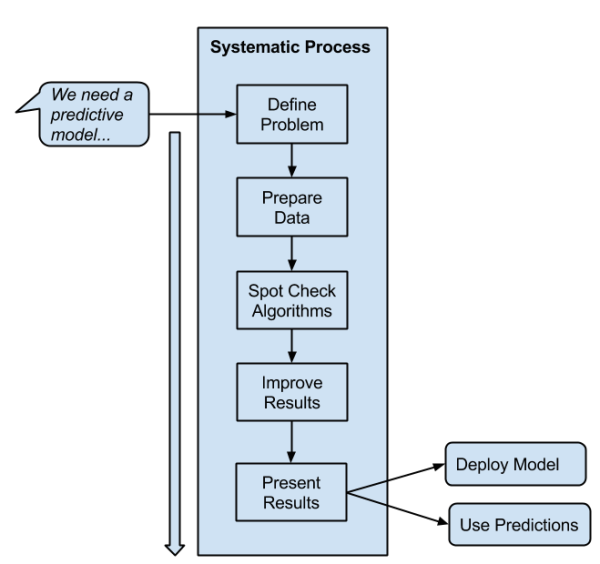
\includegraphics[height=9.5cm]{img/machine_learning_in_bioinf.png}
\caption[Common deep learning application development steps]{Common deep learning application development steps. From machinelearningmastery.com \label{fig_deep_learning_step}}
\end{center}
\end{figure}
\subsection{Data preparation}
Data preparation is a step often neglected by engineers. Computer scientists tend to focus on the algorithmic aspect of the application, but a trend in deep learning is the increasing importance of having good data. 

Good data has several folds of meanings. First, good training and validation data is the key to train a good model. In general, in deep learning, the more data the better. However, too much data also implies longer training time, so it is also a trade off. Training data should be clean, consistent, and obtained from trustworthy source. Second, several gold standard testing data should be picked at the beginning of the development cycle. Enough attention should be focused on selecting good independent testing dataset. This includes using benchmark testing dataset from previous publications or design your own testing dataset.  Third, data similarities should be checked carefully at the very beginning. The training and validation data should be filtered to contain no similarities to testing data. There should also be no similarities between and among training and validation data. Many high impact publications now require the submitted machine learning manuscripts to have a separate section discussing how training and testing data are dissimilar. Precious time could be wasted if reviewers are concerned about the dataset similarities. Because this could mean revisit the whole development process.

\subsubsection{Comparative analysis}
To perform comparative analysis, running competing methods is often needed. Sanity check is crucial but often omitted. Sanity check means by executing others' programs, one obtain identical result as reported in previous publications. This ensures running others' program correctly and evaluating result using same way. There are commonly seen mistake due to not having sanity checks. For example, evaluation metrics such as sensitivity, MCC are threshold dependent. That is, the original output of programs are regression values, and a threshold is needed to classify each value into a class, for instance, binding site and non-binding site. All programs should have a uniformed way of selecting the threshold (see Section \ref{sec_evaluation_scheme} as an example). Another common mistake is comparing the evaluation metrics on a complete testing dataset to the average of leave-one-out result on the same testing dataset.

\subsubsection{Improving results}
After the data is ready, trying different architectures, tuning parameters, and improving results often take several development cycles. It is worthwhile spending time on the infrastructure code. Good code infrastructure, such as scripting, clear system design, makes it easier to change sub-component and try ideas quickly. Following good coding standard and git practise will eventually save time and prevent accumulating technical debt.

Results can be improved by having better data, better features, better model architecture, better regularization (less overfitting). Besides collecting initial training data, sampling and shuffling the data also play a role in obtaining good model. The initial architecture usually comes from literature, and it servers as the baseline performance. Adding new elements that are proven to work in some other field into the baseline model is a good way to improve the performance. For example, ensemble learning and position information are shown to improve performances in areas like image classification and language translation, so modifying and applying them into a bioinformatics problem is also worth trying.

Regularization techniques such as dropout, L1/L2 are critical and effective in reducing model variance. It convenient to parameterize the regularization option in the development code for almost most layers, so we can try many of them quickly.
\section{Future Research}
For PPI sites prediction, many recent published deep learning techniques could potentially further improve the prediction performance. These include better protein sequence embedding using ELMo, the transformer architecture, graph neural network, residual architecture, more sophisticated data sampling. Benchmark data can be improved as well. Three of the testing dataset used in DELPHI are relatively old and new publications are still using them because no better ones exist. The ideas in DELPHI can be also transferred to protein binding sites prediction with other molecules such as DNA, RNA and ligand. Binding-partner specific prediction is also interesting. That is, not only the binding residues are predicted, also the biding proteins. Better features can be potential discovered. Section \ref{sec_arch_fea} shows that the newly added three features are more helpful than the architecture. 

For PPI prediction, our research lab is trying similar deep learning ideas to improve the prediction. The deep learning computational complexity of PPI prediction is higher than site precision. Quantization techniques and mixed precision could be used to accelerate the process. Classifying more specific area of PPI site could also be interesting. For example,  permanent and transient can be predicted separately \cite{perkins2010transient}. 


%% This adds a line for the Bibliography in the Table of Contents.
\addcontentsline{toc}{chapter}{Bibliography}
%% ***   Set the bibliography style.   ***
\bibliographystyle{plain} % (change according to your preference)
%%% ***   Set the bibliography file.   ***
\bibliography{reference}{}
%% ***   NOTE   ***
%% If you don't use bibliography files, comment out the previous line
%% and use \begin{thebibliography}...\end{thebibliography}.  (In that
%% case, you should probably put the bibliography in a separate file
%% and \include or \input it here).

%Appendices.
% \begin{appendices}
% \chapter{Proofs of Theorems}\label{AppA}
\myappendices{Appendix \ref{AppA} \byname{AppA}}
\begin{proof}[Proof of Theorem \ref{eipi}]
\begin{eqnarray}
e^{i\pi} &=& \cos(\pi) + i\sin(\pi)\\
&=& -1
\end{eqnarray} \qed
\end{proof}

\chapter{Second appendix}
this is second appendix

% \end{appendices}

%CV only relevant stuff... not full CV.
\addcontentsline{toc}{chapter}{Curriculum Vitae}
\chapter*{Curriculum Vitae}
\begin{table}[ht]
\begin{tabular}{ll}
\textbf{Name:} & \firstname{} \lastname\\\\
\textbf{Post-Secondary} & University of Western Ontario\\
\textbf{Education and}& London, ON, Canada\\
\textbf{Degrees:}& 2014 - 2020 Ph.D.\\\\
& University of Western Ontario\\
& London, ON, Canada\\
& 2012 - 2013 M.Sc.\\\\
& Anhui University\\
& Hefei, Anhui, China\\
& 2008 - 2012 B.Eng.\\\\
\textbf{Honours and}& Robert and Ruth Lumsden Graduate Awards\\
\textbf{Awards:}& March 2018\\\\
& Second Prize at University of Western Ontario Research in Computer Science\\
& April 2018\\\\
& First Prize at University of Western Ontario Research in Computer Science\\
& April 2017\\\\
& Society OF Graduate Student Travel Scholarship\\
& July 2017\\\\
\textbf{Related Work}& Senior Software Engineer\\
\textbf{Experience:}& Huawei Toronto Research Center\\
& 2018 - Current\\\\
& Research and Teaching assistant\\
& The University of Western Ontario\\
& 2012 - 2017\\
\end{tabular}
\end{table}
\subsubsection*{Publications:}
Li, Y. and Ilie, L., 2020. DELPHI: accurate deep ensemble model for protein interaction sites prediction, \\\\
Li, Y. and Ilie, L., 2019. Predicting Protein–Protein Interactions Using SPRINT. Protein-Protein Interaction Networks. Humana, New York, NY, 2020. 1-11.\\\\
Li, Y. and Ilie, L., 2017. SPRINT: ultrafast protein-protein interaction prediction of the entire human interactome. BMC bioinformatics 18.1 (2017): 485.

\subsubsection*{Referred Conference Presentations:}
DELPHI: accurate deep ensemble model for protein interaction sites prediction
(ISMB’20), 3DSIG, Montreal, 2020. (abstract and poster)\\\\
Y. Li, L. Ilie, SPRINT: Ultrafast protein-protein interaction prediction of the entire human interactome, 25th Annual International Conference on Intelligent Systems for Molecular Biology
(ISMB’17), 3DSIG, Prague, 2017. (poster)


\end{spacing}
\end{document}

